\chapter{Introduction}\label{introduction}

This thesis presents an execution stack for neural networks using the
\emph{Kubernetes}\footnote{https://kubernetes.io} container
orchestration and a Java based microservice architecture, which is
exposed to users and other systems via RESTful web services and a web
frontend. The whole workflow including importing, training and
evaluating a neural network model, becomes possible by using this
service oriented approach (SOA). The presented stack runs on popular
cloud platforms, like \emph{Google Cloud Platform}\footnote{https://cloud.google.com/kubernetes-engine},
\emph{Amazon AWS}\footnote{https://aws.amazon.com/eks} and
\emph{Microsoft Azure}\footnote{https://azure.microsoft.com/services/container-service}.
Furthermore it is scalable and each component is extensible and
interchangeable. This work is influenced by N2Sky \cite{schikuta_2013},
a framework to exchange neural network specific knowledge and aims to
support \emph{ViNNSL}, the Vienna Neural Network Specification Language
\cite{kopica_2015} \cite{beran_2008}.

\paragraph{Objectives:}\label{objectives}

The first objective is to specify functional and non-functional
requirements for the neural network system. This is followed by the
characterisation of the API and the implemention of microservices that
later define the neural network composition as a collection of loosly
coupled services.

The next step is to setup a \emph{Kubernetes} cluster to create the
foundation of container orchestration.

Finally the microservices are deployed to containers and combined in a
cluster.

\paragraph{Non-Objectives:}\label{non-objectives}

The prototype does not fully implement the \emph{ViNNSL} in version 2.0,
as described in \cite{kopica_2015} and provides limited data in-/output.
Limitations are described in section TODO.

\section{Problem Statement}\label{problem-statement}

Getting started with machine learning and in particular with neural
networks is not a trivial task. It is a complex field with a high entry
barrier and most often requires programming skills and expertise in
neural network frameworks. In most cases a complex setup is needed to
train and evaluate networks, which is both, a processor- and
memory-intense job. With cloud computing getting more and more
affordable and powerful, it makes sense to shift these tasks into the
cloud. There are already existing cloud platforms for machine learning,
but to my present research all of them do not fulfil at least one of the
following criteria:

\begin{itemize}
\tightlist
\item
  platform is open-source
\item
  no programming skills required to define and train a neural network
  model
\item
  can be deployed on-site and and in the cloud (of your choice)
\item
  components extensible and replaceable by developers
\item
  provides a RESTful interface
\end{itemize}

This thesis showcases an architecture, that tries to achieve all of
that.

\section{Motivation}\label{motivation}

Machine learning has become a highly discussed topic in information
technology in the past years and the trend is further increasing. It has
become an essential part of everyday life when using search engines or
speech recognition systems, like personal assistants. Self-learning
algorithms in applications learn from the input of their users and
decide which news an individual should read next, which song to listen
to or which social media post should appear first. Messages are being
analyzed and possible answers automatically predicted.

A recent Californian study shows that 6.5 million developers worldwide
are currently involved in projects that use artificial intelligence
techniques and another 5.8 million developers expect to implement these
in near future \cite{evans}.

Machine learning is not just a business area in the United States.
Survey results of 264 companies in the DACH region show, that 56 of them
already use that kind of technology in production. In the near future
112 companies plan to do so or already have initial experiences (see
figure \ref{img.crisp_ml_verbreitung}). It is seen by a fifth of the
decision-makers as a core area to improve the competitiveness and
profitability of companies in future. \cite{crisp}

\begin{figure}
\centering
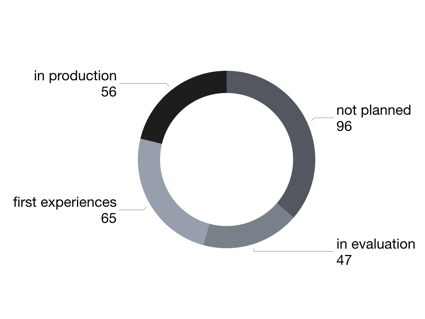
\includegraphics[width=10.00000cm]{images/crisp_ml_verbreitung}
\caption{Distribution of machine learning of 264 companies in the DACH
region \cite{crisp}\label{img.crisp_ml_verbreitung}}
\end{figure}

At the same time more and more companies shift their business logic from
a monolithic design to microservices. Each service is dedicated to a
single task that can be developed, deployed, replaced and scaled
independently. Test results have shown that not only this architecture
can help reduce infrastructure costs
\cite{villamizar2}\cite{villamizar}, but also reduces complexity of the
code base and enables applications to dynamically adjust computing
resources on demand \cite{villamizar}.

The presented project combines these techniques and demonstrates a
prototype that is open-source and supported by common cloud providers.
Developers can integrate their own solutions into the platform or
exchange components ad libitum.

It also integrates with ViNNSL, a descriptive language that does not
require programming skills to define, train and evaluate neural
networks.

\section{Structure}\label{structure}

This thesis gives an introduction and comparison to state of the art
technologies that support the microservice architecture pattern using
container and container orchestration tools. This is followed by the
acquaintance of Machine Learning (ML) and commonly used ML Frameworks.
Featuring all these introduced technologies, requirements are defined
for the implementation of a prototype. Main sections of this thesis are
the specification, implementation and documentation of the prototype
following common practices. To demonstrate the operational purposes of
the prototype, two use cases are presented.

Future work mentions ideas on how the prototype can be extended and
integrated into other systems and the conclusion summarizes the
motivation and archivements of the implemented neural network execution
stack.

\section{Related Work}\label{related-work}

\subsection{ViNNSL}\label{vinnsl}

The Vienna Neural Network Specification Language (\emph{ViNNSL}) is a
domain specific language developed by the \emph{University of Vienna} to
describe neural network objects and is designed as a communication
framework in service-oriented architectures. It is based on XML and
provides the schemas that allow the creation, training and evaluation of
artificial neural networks. \cite{beran_2008}

\subsection{N2Sky}\label{n2sky}

\emph{N2Sky} is a cloud-based platform developed by the \emph{University
of Vienna} that follows the Neural Networks as a Service paradigm and
provides an implementation example of \emph{ViNNSL}. It is designed as
virtual collaboration platform allowing to exchange neural network
knowledge with a neural network community. The service delivers an
interface to create and train neural network objects and subsequently
share them with the community. \cite{schikuta_2013}\cite{n2sky-2}

\chapter{State of the Art}\label{state-of-the-art}

\section{Containers}\label{containers}

\subsection{Docker Containers}\label{docker-containers}

Containers enable software developers to deploy applications that are
portable and consistent across different environments and providers
\cite{baier-kub} by running isolated on top of the operating system's
kernel \cite{bashari}. As an organisation, Docker\footnote{https://docker.com}
has seen an increase of popularity very quickly, mainly because of its
advantages compared to other solutions, which are speed, portability,
scalability, rapid delivery and density \cite{bashari}.

Building a Docker container is fast, because images do not include a
guest operating system. The container format itself is standardized,
which means that developers just have to ensure that their application
runs inside the container, which is then bundled into a single unit. The
unit can be deployed on any Linux system as well as on various cloud
environments and therefore easily be scaled. Not using a full operating
system makes containers use less resources than virtual machines, which
ensures higher workloads with greater density. \cite{joy2015}

\section{Microservices}\label{microservices}

The micoservice architecture pattern is a variant of a service-oriented
architecture (SOA). An often cited definition originates from Martin
Fowler and James Lewis:

\begin{quote}
In short, the microservice architectural style is an approach to
developing a single application as a suite of small services, each
running in its own process and communicating with lightweight
mechanisms, often an HTTP resource API. These services are built around
business capabilities and independently deployable by fully automated
deployment machinery. There is a bare minimum of centralized management
of these services, which may be written in different programming
languages and use different data storage technologies.
\cite{lewis2014microservices}
\end{quote}

Figure \ref{monolithic_vs_microservice} shows the architectural
difference between the monolithic and microservice architecture.
Monolithic applications bundle user interface, data access layer and
business logic together as a single unit. In the microservice
architecture each task has its own service. The user interface puts
information together from multiple services.

\begin{figure}
\centering
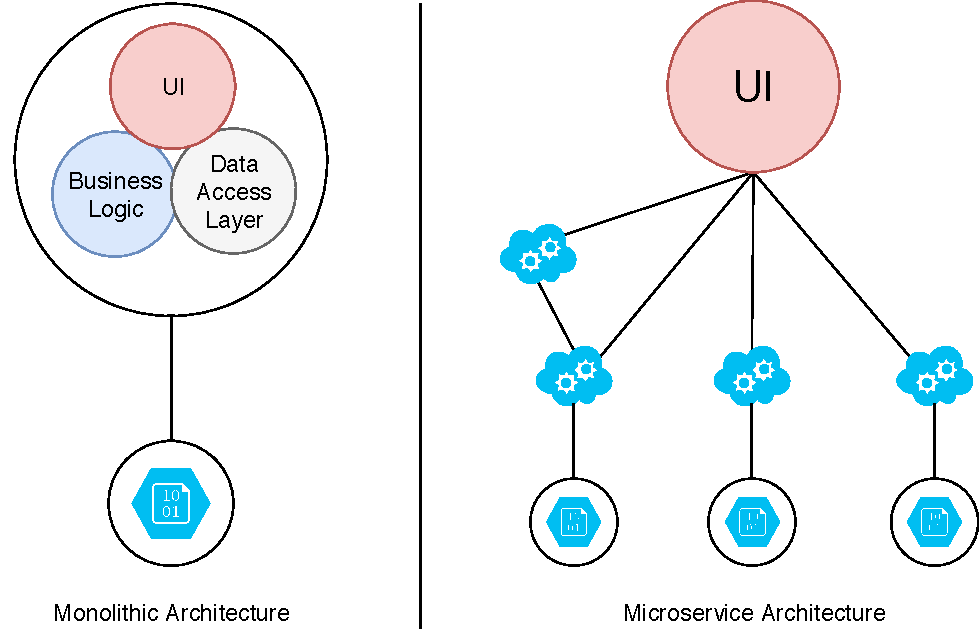
\includegraphics[width=15.00000cm]{images/monolithic_vs_microservice}
\caption{Monolithic Architecture vs.~Microservice Architecture
\label{monolithic_vs_microservice}}
\end{figure}

\section{Container Orchestration
Technologies}\label{container-orchestration-technologies}

As every single microservice runs as a container, we need a tool to
manage, organise and replace these containers. Services should also be
able to speak to each other and restarted if they fail. Services under
heavy load should be scaled for better performance. To deal with these
challenges container orchestration technologies come into place.
According to a study from 2017 published by Portworx, Kubernetes is the
most frequently used container orchestration tool in organizations,
followed by Docker Swarm and Amazon ECS. \cite{portworx-2017}

This section describes the architecture of the mentioned container
orchestration technologies and compares them.

\subsection{Kubernetes}\label{kubernetes}

Kubernetes is the third container-management system (after Borg and
Omega) developed by Google \cite{Burns:2016uq} for administering
applications, that are provided in containers, in a cluster of nodes.
Services that are responsible for controlling the cluster, are called
master components \cite{kub_intro}. Figure
\ref{kubernetes_core_architecture} shows the Kubernetes core
architecture, which includes the Master server, the nodes and the
interaction between the components.

\begin{figure}
\centering
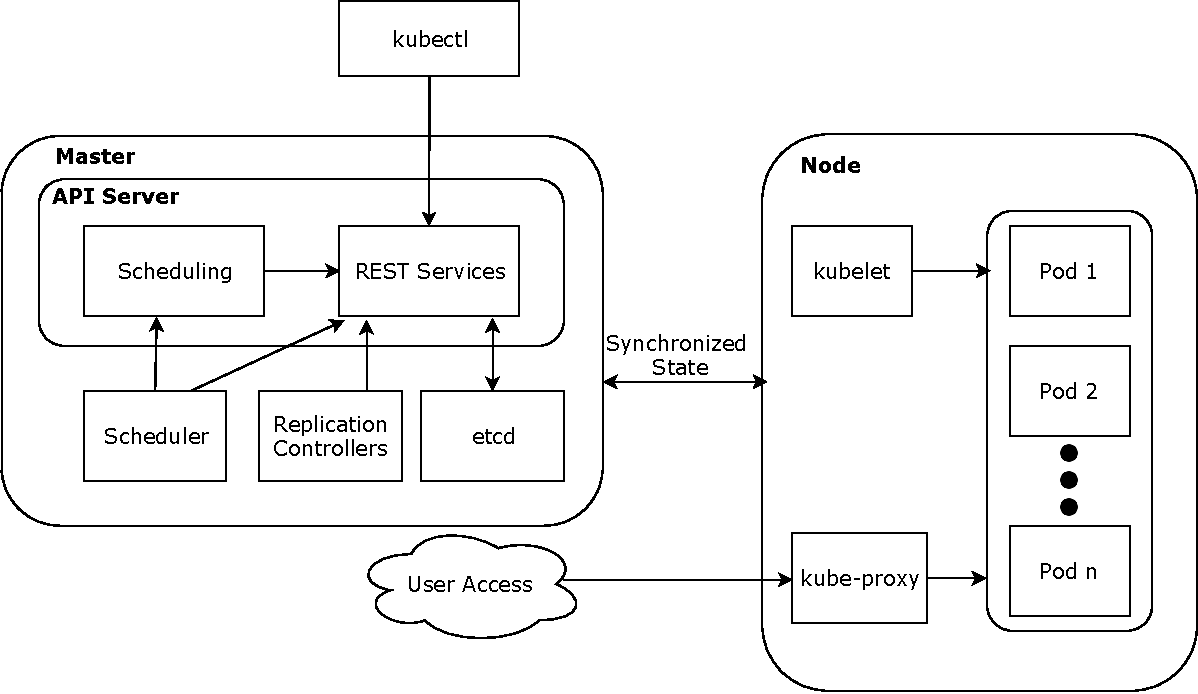
\includegraphics[width=15.00000cm]{images/kubernetes_core_architecture}
\caption{Kubernetes core
architecture\label{kubernetes_core_architecture} \cite{baier-kub}}
\end{figure}

\subsubsection{Master Components}\label{master-components}

The master consists of the core API server, that provides information
about the cluster and workload state and allows to define the desired
state \cite{baier-kub}. The master server also takes care of scheduling
and scaling workloads, cluster-wide networking and performs health
checks \cite{kub_intro}. Workloads are managed in form of so-called
pods, which are various containers that conclude the application stacks
\cite{baier-kub}.

\paragraph{etcd}\label{etcd}

etcd is a key-value store, accessible by a HTTP/JSON API, which can be
distributed across multiple nodes and is used by Kubernetes to store
configuration data, which needs to be accessible across nodes deployed
in the cluster. It is essential for service discovery and to describe
the state of the cluster, among other things. \cite{kub_intro}

etcd can also watch values for changes \cite{baier-kub}.

\paragraph{kube-apiserver}\label{kube-apiserver}

The API server acts as the main management point for the cluster and
provides a RESTful interface for users and other services to configure
workloads in the cluster. It is a bridge between other master components
and is responsible of maintaining health and spreading commands in the
cluster. \cite{kub_intro}

\paragraph{kube-scheduler}\label{kube-scheduler}

The scheduler keeps track of available and allocated resources on each
specific node in the cluster. It has an overview of the infrastructure
environment and needs to distribute workload to an acceptable node
without exceeding the available resources. Therefore each workload has
to declare its operating requirements. \cite{kub_intro}

\paragraph{kube-controller-manager}\label{kube-controller-manager}

The controller manager mainly operates different controllers that
constantly check the shared state of the cluster in \texttt{etcd} via
the apiserver \cite{kub_comp} and if the current state differs towards
the desired state it takes compensating measures \cite{kub_intro}.

For example the node controller's task is to react when nodes go offline
or down. The replication controller makes sure that the defined number
of desired pods is identical to the number of currently deployed pods in
the cluster and scales applications up or down accordingly. The
endpoints controller populates the endpoints to services \cite{kub_comp}

\paragraph{cloud-controller-manager}\label{cloud-controller-manager}

Kubernetes supports different cloud infrastructure providers. As each
cloud providers has different features, apis and capabilities, cloud
controller managers act as an abstraction to the generic internal
Kubernetes constructs. This has the advantage that the core Kubernetes
code is not dependent on cloud-provider-specific code. \cite{kub_comp}

\subsubsection{Node Components}\label{node-components}

Servers that accomplish workloads are called nodes. Each workload is
described as one or more containers that have to be deployed. Node
components run on every node in the cluster providing the Kubernetes
runtime environment \cite{kub_comp}, that establishes networking and
communicates with the master components. They also take care of
deploying the necessary containers on a node and keep them running
\cite{kub_intro}. Kubernetes requires a dedicated subnet for each node
server and a supported container runtime \cite{kub_comp}.

\paragraph{kubelet}\label{kubelet}

The kubelet is the primary agent running on each node in the cluster,
responsible for running pods \cite{kub_comp}. It communicates with the
API server to receive commands invoked by the scheduler. Interaction
takes place with the etcd store to read and update configuration and
state of the pod.

Pods are specified by the \emph{PodSpec}, which defines the workload and
parameters on how to run the containers \cite{kub_intro}. The kubelet
process is responsible that the containers described in the
specification are running and healthy \cite{kub_comp}.

\paragraph{kube-proxy}\label{kube-proxy}

The proxy service is in charge of forwarding requests of defined
services to the correct containers. On a basic level, load balancing is
also done by the proxy. \cite{baier-kub}

\paragraph{Container Runtime}\label{container-runtime}

The container runtime is an implementation running containers. Currently
Docker, rkt, runc and OpenContainer runtimes are supported.
\cite{kub_comp}

\paragraph{Pods}\label{pods}

A pod is the smallest deployable unit in a cluster consisting of a group
of one or more containers, which share network and storage.
\cite{kub-pod}

\subsubsection{Addons}\label{addons}

\paragraph{Cluster DNS}\label{cluster-dns}

Cluster DNS server keeps track of running services in the cluster and
updates DNS records accordingly. This allows an easy way of service
discovery. Containers include this DNS server in their DNS lookups
automatically -- that way a service can resolve another service by its
name. \cite{baier-kub}

\paragraph{Ingress}\label{ingress}

Ingress handles the traffic from outside the cluster and forwards it to
the correct service using the dns service acting as a proxy server.
Currently there are two official implementations: \texttt{ingress-gce}
and \texttt{ingress-nginx}. \emph{Ingress} also provides basic load
balancing. \cite{kub-ingress}

\paragraph{Dashboard}\label{dashboard}

The dashboard is a web-based user interface that allows to manage
\emph{Kubernetes} clusters and applications running in the cluster
\cite{kub_comp}. It also provides access to log messages in each pod.

\subsubsection{Minikube}\label{minikube}

Minikube is a tool to run a single-node Kubernetes cluster locally on
computers supporting various virtual machine drivers.

\subsection{Docker Swarm Mode}\label{docker-swarm-mode}

\emph{Docker Swarm Mode} is the successor of \emph{Docker Swarm} and
implements a cluster management and orchestration tooling directly built
into \emph{Docker}\footnote{https://docker.com} .

\subsubsection{Components}\label{components}

Docker hosts can run in swarm mode, a swarm consists of one or mode
hosts that act as managers and workers. Hosts can be managers, which
means delegators of work, or workers, that run services, or both.
\cite{dock-swarm}

\paragraph{Service}\label{service}

Services are definitions of tasks that will be executed on manager or
worker nodes, specified by which container image to use and which
commands to execute \cite{dock-swarm}.

A service has attributes attached to it, that define its optimal state.

Services can be replicated, attached to storage and network resources
and expose ports to the outside, defined by attributes. You can change
the attributes while runtime, without restarting a service.
\cite{dock-swarm}

\paragraph{Task}\label{task}

A task is a running container itself which is assigned to the service.
It is managed by the \emph{swarm manager}. Manager nodes assign tasks to
worker nodes, respecting the service scale.\cite{dock-swarm}

\paragraph{Nodes}\label{nodes}

A node is a Docker instance that is a participant in the the
\emph{swarm}. Nodes are typically typically distributed across multiple
physical machines (in the cloud), but can also run on a single computer.
\cite{dock-swarm}

\paragraph{Manager Nodes}\label{manager-nodes}

Manager nodes are responsible for deploying applications and dispatching
tasks to worker nodes. Secondly one elected leader manager node
supervises functions to maintain the desired state of the swarm (defined
by the service). \cite{dock-swarm}

\paragraph{Worker nodes}\label{worker-nodes}

Worker nodes execute tasks from the manager nodes and notifies them
about the current state of its tasks.\cite{dock-swarm}

\paragraph{Load balancing \& DNS}\label{load-balancing-dns}

Like Kubernetes, the swarm manager uses ingress to expose and load
balance services.

An internal DNS component assigns each service a DNS entry
automatically. \cite{dock-swarm}

\subsubsection{Announcements}\label{announcements}

On October 17, 2017 at the conference \emph{DockerCon}\footnote{https://europe-2017.dockercon.com/},
Docker announced that it would integrate Kubernetes into the Docker
platform.

\subsection{Comparison}\label{comparison}

\subsubsection{Community}\label{community}

The following table shows a comparison of publicly available metrics on
\emph{GitHub}, trying to represent community interest in the previously
mentioned orchestrator softwares. Both projects are open-sourced and
released under the \emph{Apache-2.0}\footnote{http://www.apache.org/licenses/LICENSE-2.0}
license. These metrics were collected on June 21, 2018 and are rounded
to the nearest ten. Comparing the numbers it can be assumed that the
open-source community has currently a stronger interest in the
\emph{Kubernetes} project.

\begin{longtable}[]{@{}lll@{}}
\toprule
& Kubernetes \footnote{https://github.com/kubernetes/kubernetes} &
Docker Swarm Mode \footnote{https://github.com/docker/swarm}\tabularnewline
\midrule
\endhead
Contributors & 1.700 & 165\tabularnewline
Commits & 66.820 & 3.530\tabularnewline
Stars & 37.830 & 5.150\tabularnewline
Forks & 13.220 & 1.060\tabularnewline
\bottomrule
\end{longtable}

\subsubsection{Feature Differentiation}\label{feature-differentiation}

The handling of \emph{Docker Swarm Mode} and Kubernetes is similar in
many aspects, like load balancing with Ingress, service discovery via
DNS, and the definition language YAML. Auto-scaling, which means
increasing or decreasing running instances of a service as the load
changes over time, is not directly available in \emph{Docker Swarm
Mode}, in contrast to Kubernetes.

\emph{Docker Swam Mode} provides the possibility to mount local volumes
or folders into a container. Kubernetes has two APIs available: Volumes
and Persistent Volumes. Volumes are an abstraction with several
different implementations for cloud storages (like AWS, Azure) and are
bound to the lifecycle of a pod. Once a pod is removed, also the volume
data is gone. Persistent Volumens allow data to be persisted
independently from a pod.

Both technologies provide an easy to install development environment,
Kubernetes is available via the minikube package as well as in the
newest version of Docker Community Edition. Docker Swarm Mode is also
available via the Docker application.

\subsection{Decision}\label{decision}

Taking into account the community size, the feature-richness and the
out-of-the-box support by the major players Amazon AWS, Microsoft Azure
and Google Cloud Engine, Kubernetes is the selected technology for the
presented execution stack.

\section{Machine Learning}\label{machine-learning}

The term \emph{machine learning} originates from a 1959 article by
Arthur Samuel \cite{Samuel59somestudies} presenting a method how
computers can learn to play a better game of checkers than human.

Today, a research area within artificial intelligence, it is generally
known as the process that trains computers to improve performance
specific tasks through exposure to data, rather than through explicit
programming by using statistical techniques. It is used to conceive
complex models that lead themselves to prediction.

There are different approaches to machine learning, like decision trees
or predicition rules \cite{michalski2013machine}. This thesis focuses on
neural networks.

\section{Neural Networks}\label{neural-networks}

Neural networks, or more correctly artificial neural networks, are
derived from the neural system of the human brain. Neurons are the basic
element of the nervous system and can be divided into three essential
features: the dendrites, the soma and the axon. The human brain consists
of about 10 billon neurons, which communicate through a network of axons
and synapses. Artificial neural networks try to imitate this connection.
\cite{haun1998simulation}

\subsection{Classification of Neural
Networks}\label{classification-of-neural-networks}

Figure \ref{nn_class_haun} shows a classification of neural networks by
Haun \cite{haun1998simulation} divided into three levels based on
connection type, neuronal behavior and learning methods. The first level
classifies into feedback and feedforward networks.

\subsubsection{Feedforward networks}\label{feedforward-networks}

Feedforward networks consist of connections in one direction only.
Neurons are connected between different layers and normally spread from
input to output through hidden layers. The output can be calculated from
the input directly. Loops are not allowed \cite{haun1998simulation}.

TODO Figure

\paragraph{Linear and non-linear
networks}\label{linear-and-non-linear-networks}

Linear networks use linear activation functions. The output of a neuron
is bound directly to the value of activation function. Non-linear
networks use non-linear activation functions, which means that the
activation value is one, if the sum of all input values exceed a
threshold value, otherwise it is zero. \cite{haun1998simulation}

A Perceptron network is for example a linear network.

\paragraph{Supervised and unsupervised
networks}\label{supervised-and-unsupervised-networks}

Supervised networks compare its output values with the correct answer
during training and continuously adapt input values to approximate both
values. Unsupervised networks do not have such information and must
learn through an inherent mechanism. It is presumed that impulses and
reactions relate in a way that produces correct behaviour after the
learning period is finished. \cite{haun1998simulation}

\subsubsection{Feedback networks}\label{feedback-networks}

Feedback networks are networks where neurons are also connected between
different layers, but the output of a neuron can connected with an input
of other neuron. Output values are therefore dependant from previous
input values of the neural network. \cite{haun1998simulation}

TODO Figure

\paragraph{Defined constructed
networks}\label{defined-constructed-networks}

asdf

\paragraph{Trained networks}\label{trained-networks}

\begin{figure}
\centering
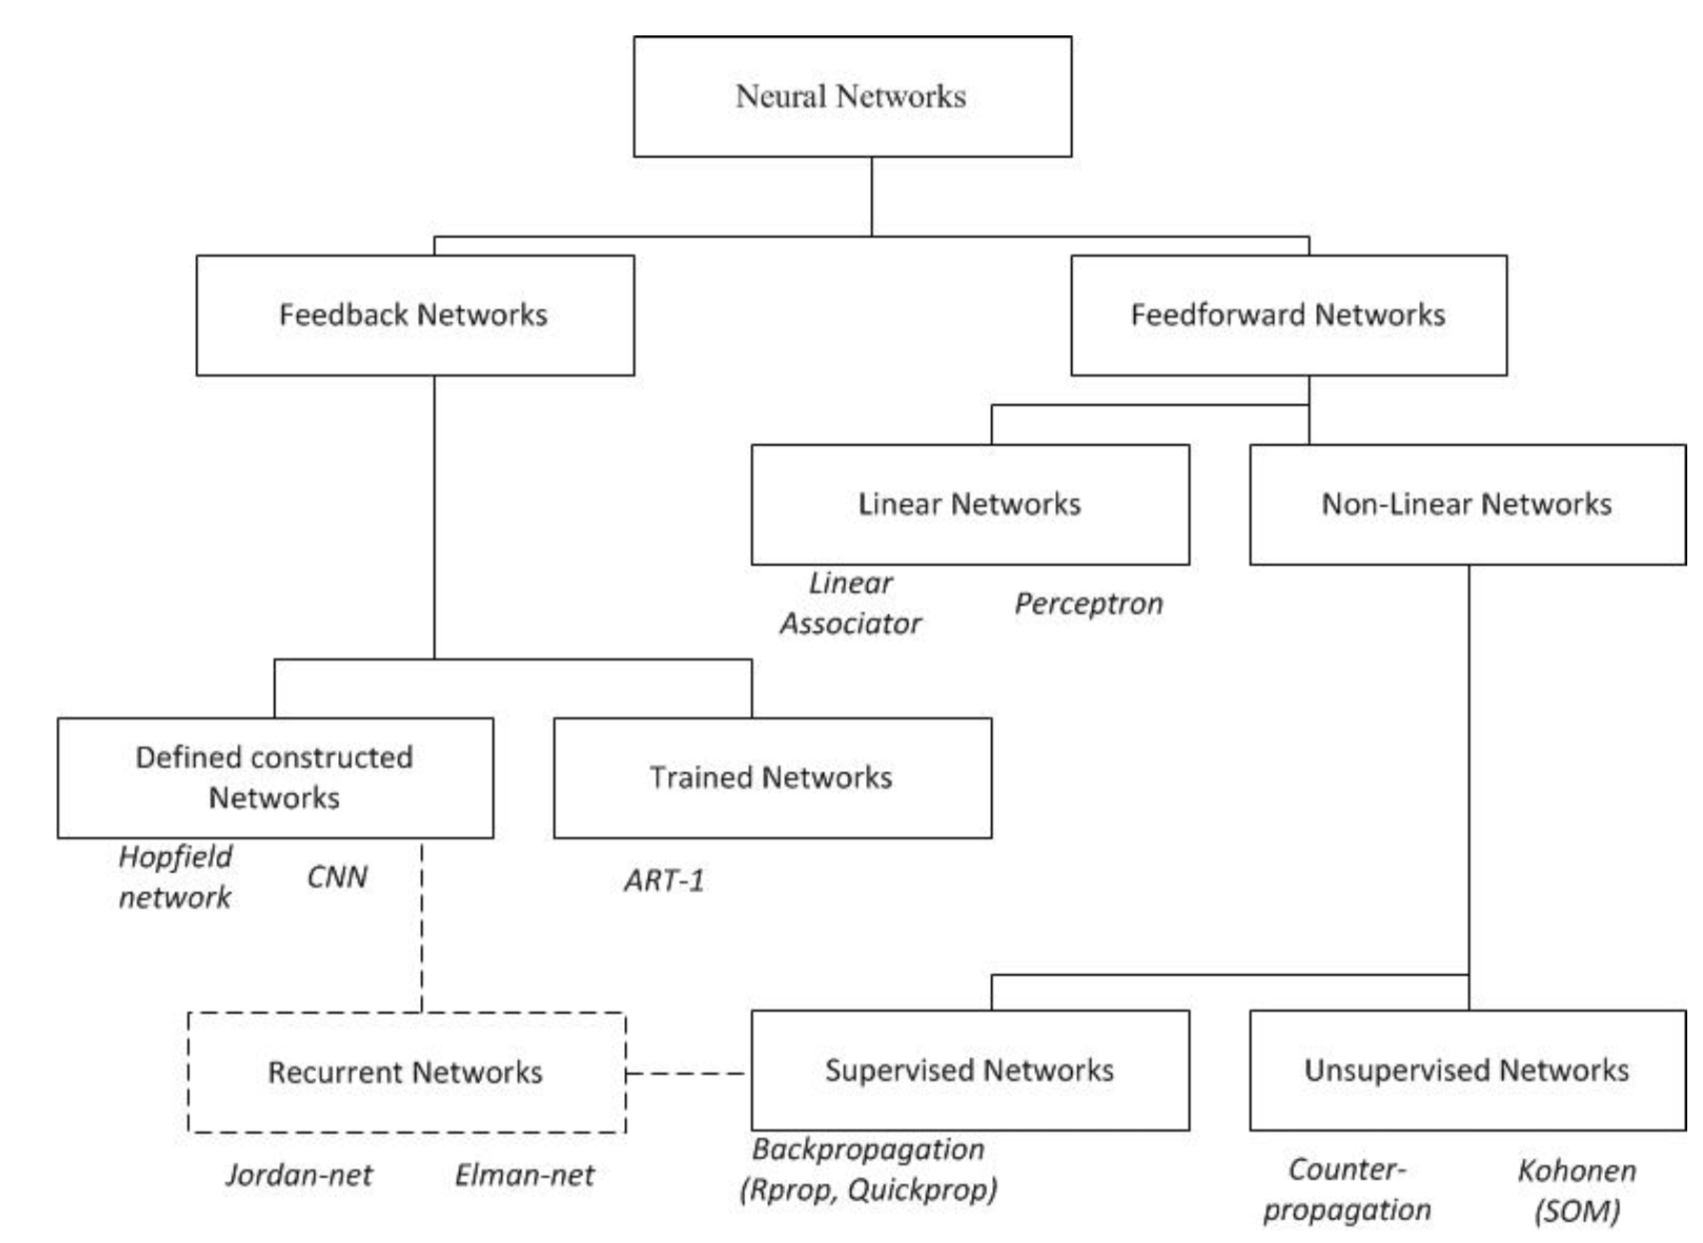
\includegraphics[width=15.00000cm]{images/nn_class_haun}
\caption{Classification of neural networks by Haun
\cite{haun1998simulation} \label{nn_class_haun}}
\end{figure}

\subsection{Backpropagation}\label{backpropagation}

\subsection{Neural Network Frameworks}\label{neural-network-frameworks}

Neural network frameworks

\subsubsection{Tensorflow}\label{tensorflow}

Tensorflow is an open-sourced framework that was developed by the
\emph{Google Brain Team} as successor to the proprietary software
DistBelief. It is an interface and implementation for machine learning
algorithms featuring support for a wide range of devices and GPU cards.
\cite{dean-tensor}

\subsubsection{Deeplearning4J}\label{deeplearning4j}

\chapter{Requirements}\label{requirements}

This section defines functional and non-functional requirements for the
developed prototype. The neural network execution stack focuses on two
main target groups: data scientists and developers.

Data scientists use the provided services in a deployed environment
(cloud or own computer) to develop and train their neural networks. The
system should be easy to setup and no programming knowledge should be
needed to get started.

Developers can extend the neural network stack with features or use the
provided web services to implement their own custom solution.

\section{Functional Requirements}\label{functional-requirements}

Due to the fact that neural network training requires a lot of computing
power, the main requirement is to design an architecture that can be
executed in the cloud or on-site cluster hardware.

To enable developers to extend the application, it is designed as a
platform that is open-sourced and documented. An easy setup on a local
computer and small micro-services with a clear structure and manageable
code base make it easier to get acquainted with the architecture.

The neural network platform should also offer a way to be extended or
used by external applications and services, therefore a documented
RESTful webservice is provided, that can be consumed by various clients.

\subsection{User Interface}\label{user-interface}

The user interface shall be a web application that gives a quick
overview of all neural networks and their training status. The frontend
uses the RESTful API as backend source and does not cover the whole
function range of the API.

\subsubsection{Mockup}\label{mockup}

Figure \ref{vinnsl-ui-mockup} shows a sketch of the user interface. On
the left side the user can see a list of all created or imported neural
networks. Next to the names of the networks, there is an icon
representing the training status. In the detailed view on the right
side, the title and id of the network is shown followed by an indicator
when training is in progress. The visualisation of a neural network is
divided into tabs.

The tabs ``Description'', ``Definition'', ``Instance'' and ``Result''
represent the eponymous ViNNSL Description XML file into a graphical
tree view. When enough information is provided by ViNNSL XML files, the
worker service performs a transformation into the internally used model
representation of the \emph{Deeplearning4J} Framework. The
\emph{Deeplearning4J} Tab shows the transformed object. In the ``Files''
tab, imported files of the storage services are listed and can be
selected as training- or testset.

\begin{figure}
\centering
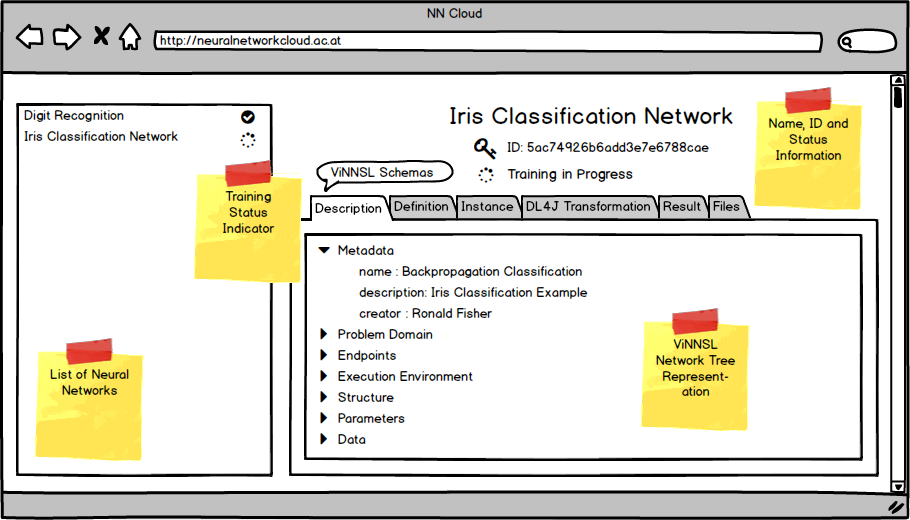
\includegraphics[width=17.00000cm]{./images/vinnsl-ui-mockup}
\caption{Mockup: User Interface of Frontend
Service\label{vinnsl-ui-mockup}}
\end{figure}

\section{Non-Functional Requirements}\label{non-functional-requirements}

\subsection{Quality}\label{quality}

The execution stack shall comply with the following quality features:

\begin{itemize}
\tightlist
\item
  Standard RESTful API
\item
  the user interface works on all common browsers and devices
  (responsive design)
\item
  loading time of the user interface should be less than three seconds
\end{itemize}

\subsection{Technical}\label{technical}

\subsection{Software}\label{software}

\begin{itemize}
\tightlist
\item
  Kubernetes
\item
  Docker
\item
  Java Standard Platform
\item
  Maven Plugin for Java
\end{itemize}

\subsection{Hardware}\label{hardware}

\begin{itemize}
\tightlist
\item
  Kubernetes compatible hardware or Cloud account (Amazon Web Services,
  Google Cloud Engine)
\end{itemize}

\subsection{Documentation}\label{documentation}

The documentation is provided in Section
\ref{prototype-api-documentation} or online on SwaggerHub\footnote{https://app.swaggerhub.com/apis/a00908270/}.

\subsection{Source Code}\label{source-code}

The source code is released on GitHub \footnote{https://github.com/a00908270/}.

\subsection{Developer Environment}\label{developer-environment}

Developers can use any Java Based development environment.

\chapter{Specification}\label{specification}

\section{Use Case}\label{use-case}

Figure \ref{img.use_case_nn} shows the UML use case diagram.

\begin{figure}
\centering
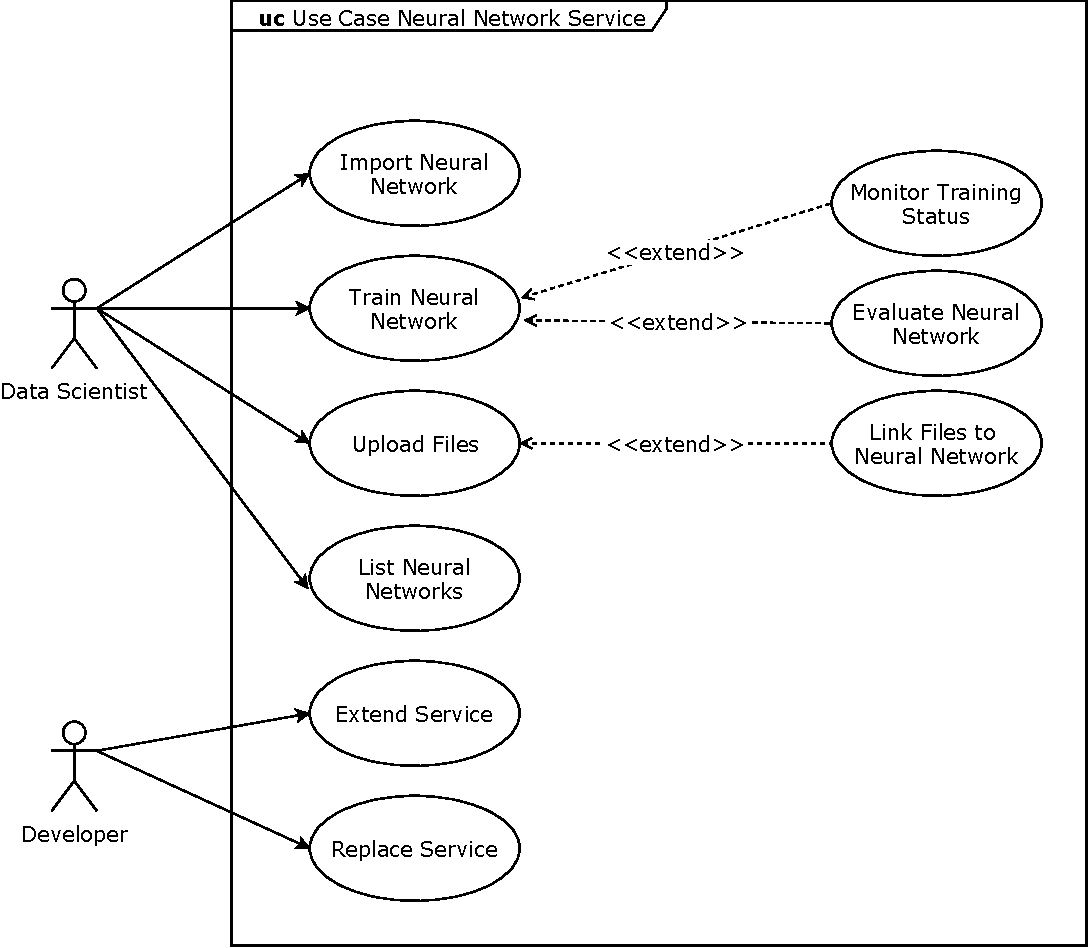
\includegraphics[width=15.00000cm]{images/use_case_nn}
\caption{UML Use Case Diagram \label{img.use_case_nn}}
\end{figure}

\subsection{Use Case Descriptions}\label{use-case-descriptions}

\begin{longtable}[]{@{}ll@{}}
\toprule
\begin{minipage}[b]{0.27\columnwidth}\raggedright\strut
\textbf{Use Case}\strut
\end{minipage} & \begin{minipage}[b]{0.68\columnwidth}\raggedright\strut
\textbf{Import Neural Network}\strut
\end{minipage}\tabularnewline
\midrule
\endhead
\begin{minipage}[t]{0.27\columnwidth}\raggedright\strut
Description\strut
\end{minipage} & \begin{minipage}[t]{0.68\columnwidth}\raggedright\strut
An existing ViNNSL XML file with a neural network description is
imported via the vinnsl web service into the database.\strut
\end{minipage}\tabularnewline
\begin{minipage}[t]{0.27\columnwidth}\raggedright\strut
Priority\strut
\end{minipage} & \begin{minipage}[t]{0.68\columnwidth}\raggedright\strut
primary\strut
\end{minipage}\tabularnewline
\begin{minipage}[t]{0.27\columnwidth}\raggedright\strut
Actors\strut
\end{minipage} & \begin{minipage}[t]{0.68\columnwidth}\raggedright\strut
Data Scientist\strut
\end{minipage}\tabularnewline
\begin{minipage}[t]{0.27\columnwidth}\raggedright\strut
Preconditions\strut
\end{minipage} & \begin{minipage}[t]{0.68\columnwidth}\raggedright\strut
ViNNSL neural network XML description file\strut
\end{minipage}\tabularnewline
\begin{minipage}[t]{0.27\columnwidth}\raggedright\strut
Postconditions\strut
\end{minipage} & \begin{minipage}[t]{0.68\columnwidth}\raggedright\strut
---\strut
\end{minipage}\tabularnewline
\begin{minipage}[t]{0.27\columnwidth}\raggedright\strut
Normal Course of Events\strut
\end{minipage} & \begin{minipage}[t]{0.68\columnwidth}\raggedright\strut
* The actor sends a POST request to the ViNNSL web service including a
XML body* The web service validates and imports the XML file and returns
the HTTP status code 201 CREATED\strut
\end{minipage}\tabularnewline
\begin{minipage}[t]{0.27\columnwidth}\raggedright\strut
Alternative Courses\strut
\end{minipage} & \begin{minipage}[t]{0.68\columnwidth}\raggedright\strut
* The post request is sent by an application or other service\strut
\end{minipage}\tabularnewline
\begin{minipage}[t]{0.27\columnwidth}\raggedright\strut
Exceptions\strut
\end{minipage} & \begin{minipage}[t]{0.68\columnwidth}\raggedright\strut
If the validation fails or an error occurs, the web service returns the
HTTP status code 500\strut
\end{minipage}\tabularnewline
\begin{minipage}[t]{0.27\columnwidth}\raggedright\strut
Assumptions\strut
\end{minipage} & \begin{minipage}[t]{0.68\columnwidth}\raggedright\strut
Access to the \texttt{vinnsl-service}\strut
\end{minipage}\tabularnewline
\bottomrule
\end{longtable}

\begin{longtable}[]{@{}ll@{}}
\toprule
\begin{minipage}[b]{0.27\columnwidth}\raggedright\strut
\textbf{Use Case}\strut
\end{minipage} & \begin{minipage}[b]{0.68\columnwidth}\raggedright\strut
\textbf{Train Neural Network}\strut
\end{minipage}\tabularnewline
\midrule
\endhead
\begin{minipage}[t]{0.27\columnwidth}\raggedright\strut
Description\strut
\end{minipage} & \begin{minipage}[t]{0.68\columnwidth}\raggedright\strut
An imported neural network is trained by passing the configuration over
to the worker service.\strut
\end{minipage}\tabularnewline
\begin{minipage}[t]{0.27\columnwidth}\raggedright\strut
Priority\strut
\end{minipage} & \begin{minipage}[t]{0.68\columnwidth}\raggedright\strut
primary\strut
\end{minipage}\tabularnewline
\begin{minipage}[t]{0.27\columnwidth}\raggedright\strut
Actors\strut
\end{minipage} & \begin{minipage}[t]{0.68\columnwidth}\raggedright\strut
Data Scientist\strut
\end{minipage}\tabularnewline
\begin{minipage}[t]{0.27\columnwidth}\raggedright\strut
Preconditions\strut
\end{minipage} & \begin{minipage}[t]{0.68\columnwidth}\raggedright\strut
Imported ViNNSL neural network XML description, definition and instance
file\strut
\end{minipage}\tabularnewline
\begin{minipage}[t]{0.27\columnwidth}\raggedright\strut
Postconditions\strut
\end{minipage} & \begin{minipage}[t]{0.68\columnwidth}\raggedright\strut
---\strut
\end{minipage}\tabularnewline
\begin{minipage}[t]{0.27\columnwidth}\raggedright\strut
Normal Course of Events\strut
\end{minipage} & \begin{minipage}[t]{0.68\columnwidth}\raggedright\strut
* The actor sends a POST request to the working service including the
identifier of the neural network that should be trained* The webservice
validates the request, adds the network into the training queue and
returns the HTTP status code 200.\strut
\end{minipage}\tabularnewline
\begin{minipage}[t]{0.27\columnwidth}\raggedright\strut
Alternative Courses\strut
\end{minipage} & \begin{minipage}[t]{0.68\columnwidth}\raggedright\strut
* The post request is sent by an application or other service\strut
\end{minipage}\tabularnewline
\begin{minipage}[t]{0.27\columnwidth}\raggedright\strut
Exceptions\strut
\end{minipage} & \begin{minipage}[t]{0.68\columnwidth}\raggedright\strut
If the validation fails or an error occurs, the webservice returns the
HTTP statuscode 500\strut
\end{minipage}\tabularnewline
\begin{minipage}[t]{0.27\columnwidth}\raggedright\strut
Assumptions\strut
\end{minipage} & \begin{minipage}[t]{0.68\columnwidth}\raggedright\strut
Access to the \texttt{vinnsl-nn-worker}\strut
\end{minipage}\tabularnewline
\begin{minipage}[t]{0.27\columnwidth}\raggedright\strut
Extensions\strut
\end{minipage} & \begin{minipage}[t]{0.68\columnwidth}\raggedright\strut
* Monitor Training Status * Evaluate Neural Network\strut
\end{minipage}\tabularnewline
\bottomrule
\end{longtable}

\begin{longtable}[]{@{}ll@{}}
\toprule
\begin{minipage}[b]{0.27\columnwidth}\raggedright\strut
\textbf{Use Case}\strut
\end{minipage} & \begin{minipage}[b]{0.68\columnwidth}\raggedright\strut
\textbf{Monitor Training Status}\strut
\end{minipage}\tabularnewline
\midrule
\endhead
\begin{minipage}[t]{0.27\columnwidth}\raggedright\strut
Description\strut
\end{minipage} & \begin{minipage}[t]{0.68\columnwidth}\raggedright\strut
The Data Scientist monitors the training status to evaluate the trained
network afterwards.\strut
\end{minipage}\tabularnewline
\begin{minipage}[t]{0.27\columnwidth}\raggedright\strut
Priority\strut
\end{minipage} & \begin{minipage}[t]{0.68\columnwidth}\raggedright\strut
secondary\strut
\end{minipage}\tabularnewline
\begin{minipage}[t]{0.27\columnwidth}\raggedright\strut
Actors\strut
\end{minipage} & \begin{minipage}[t]{0.68\columnwidth}\raggedright\strut
Data Scientist\strut
\end{minipage}\tabularnewline
\begin{minipage}[t]{0.27\columnwidth}\raggedright\strut
Preconditions\strut
\end{minipage} & \begin{minipage}[t]{0.68\columnwidth}\raggedright\strut
Training of neural network started\strut
\end{minipage}\tabularnewline
\begin{minipage}[t]{0.27\columnwidth}\raggedright\strut
Postconditions\strut
\end{minipage} & \begin{minipage}[t]{0.68\columnwidth}\raggedright\strut
---\strut
\end{minipage}\tabularnewline
\begin{minipage}[t]{0.27\columnwidth}\raggedright\strut
Normal Course of Events\strut
\end{minipage} & \begin{minipage}[t]{0.68\columnwidth}\raggedright\strut
* The actor sends a GET request to the status endpoint of the vinnsl
service including the identifier of the neural network that is in
progress.* The web service validates the request, and returns the
training status along the HTTP status code 200.\strut
\end{minipage}\tabularnewline
\begin{minipage}[t]{0.27\columnwidth}\raggedright\strut
Alternative Courses\strut
\end{minipage} & \begin{minipage}[t]{0.68\columnwidth}\raggedright\strut
* The post request is sent by an application or other service\strut
\end{minipage}\tabularnewline
\begin{minipage}[t]{0.27\columnwidth}\raggedright\strut
Exceptions\strut
\end{minipage} & \begin{minipage}[t]{0.68\columnwidth}\raggedright\strut
If the validation fails or an error occurs, the web service returns the
HTTP statuscode 500\strut
\end{minipage}\tabularnewline
\begin{minipage}[t]{0.27\columnwidth}\raggedright\strut
Assumptions\strut
\end{minipage} & \begin{minipage}[t]{0.68\columnwidth}\raggedright\strut
Access to the \texttt{vinnsl-service}\strut
\end{minipage}\tabularnewline
\begin{minipage}[t]{0.27\columnwidth}\raggedright\strut
Extensions\strut
\end{minipage} & \begin{minipage}[t]{0.68\columnwidth}\raggedright\strut
---\strut
\end{minipage}\tabularnewline
\bottomrule
\end{longtable}

\begin{longtable}[]{@{}ll@{}}
\toprule
\begin{minipage}[b]{0.27\columnwidth}\raggedright\strut
\textbf{Use Case}\strut
\end{minipage} & \begin{minipage}[b]{0.68\columnwidth}\raggedright\strut
\textbf{Evaluate Neural Network}\strut
\end{minipage}\tabularnewline
\midrule
\endhead
\begin{minipage}[t]{0.27\columnwidth}\raggedright\strut
Description\strut
\end{minipage} & \begin{minipage}[t]{0.68\columnwidth}\raggedright\strut
The Data Scientist evaluates the accuracy of the network after its
training\strut
\end{minipage}\tabularnewline
\begin{minipage}[t]{0.27\columnwidth}\raggedright\strut
Priority\strut
\end{minipage} & \begin{minipage}[t]{0.68\columnwidth}\raggedright\strut
primary\strut
\end{minipage}\tabularnewline
\begin{minipage}[t]{0.27\columnwidth}\raggedright\strut
Actors\strut
\end{minipage} & \begin{minipage}[t]{0.68\columnwidth}\raggedright\strut
Data Scientist\strut
\end{minipage}\tabularnewline
\begin{minipage}[t]{0.27\columnwidth}\raggedright\strut
Preconditions\strut
\end{minipage} & \begin{minipage}[t]{0.68\columnwidth}\raggedright\strut
Training of neural network successfully finished\strut
\end{minipage}\tabularnewline
\begin{minipage}[t]{0.27\columnwidth}\raggedright\strut
Postconditions\strut
\end{minipage} & \begin{minipage}[t]{0.68\columnwidth}\raggedright\strut
---\strut
\end{minipage}\tabularnewline
\begin{minipage}[t]{0.27\columnwidth}\raggedright\strut
Normal Course of Events\strut
\end{minipage} & \begin{minipage}[t]{0.68\columnwidth}\raggedright\strut
* The actor sends a GET request to the status endpoint of the vinnsl
service including the identifier of the neural network that is
finished.* The web service validates the request, and returns the ViNNSL
XML file including the result scheme.\strut
\end{minipage}\tabularnewline
\begin{minipage}[t]{0.27\columnwidth}\raggedright\strut
Alternative Courses\strut
\end{minipage} & \begin{minipage}[t]{0.68\columnwidth}\raggedright\strut
* The post request is sent by an application or other service\strut
\end{minipage}\tabularnewline
\begin{minipage}[t]{0.27\columnwidth}\raggedright\strut
Exceptions\strut
\end{minipage} & \begin{minipage}[t]{0.68\columnwidth}\raggedright\strut
If the validation fails or an error occurs, the webservice returns the
HTTP statuscode 500\strut
\end{minipage}\tabularnewline
\begin{minipage}[t]{0.27\columnwidth}\raggedright\strut
Assumptions\strut
\end{minipage} & \begin{minipage}[t]{0.68\columnwidth}\raggedright\strut
Access to the \texttt{vinnsl-service}\strut
\end{minipage}\tabularnewline
\begin{minipage}[t]{0.27\columnwidth}\raggedright\strut
Extensions\strut
\end{minipage} & \begin{minipage}[t]{0.68\columnwidth}\raggedright\strut
---\strut
\end{minipage}\tabularnewline
\bottomrule
\end{longtable}

\begin{longtable}[]{@{}ll@{}}
\toprule
\begin{minipage}[b]{0.27\columnwidth}\raggedright\strut
\textbf{Use Case}\strut
\end{minipage} & \begin{minipage}[b]{0.68\columnwidth}\raggedright\strut
Upload Files\strut
\end{minipage}\tabularnewline
\midrule
\endhead
\begin{minipage}[t]{0.27\columnwidth}\raggedright\strut
Description\strut
\end{minipage} & \begin{minipage}[t]{0.68\columnwidth}\raggedright\strut
The Data Scientist uploads files, that are usable as datasets (f.ex. CSV
files or pictures) to the storage service\strut
\end{minipage}\tabularnewline
\begin{minipage}[t]{0.27\columnwidth}\raggedright\strut
Priority\strut
\end{minipage} & \begin{minipage}[t]{0.68\columnwidth}\raggedright\strut
primary\strut
\end{minipage}\tabularnewline
\begin{minipage}[t]{0.27\columnwidth}\raggedright\strut
Actors\strut
\end{minipage} & \begin{minipage}[t]{0.68\columnwidth}\raggedright\strut
Data Scientist\strut
\end{minipage}\tabularnewline
\begin{minipage}[t]{0.27\columnwidth}\raggedright\strut
Preconditions\strut
\end{minipage} & \begin{minipage}[t]{0.68\columnwidth}\raggedright\strut
---\strut
\end{minipage}\tabularnewline
\begin{minipage}[t]{0.27\columnwidth}\raggedright\strut
Postconditions\strut
\end{minipage} & \begin{minipage}[t]{0.68\columnwidth}\raggedright\strut
---\strut
\end{minipage}\tabularnewline
\begin{minipage}[t]{0.27\columnwidth}\raggedright\strut
Normal Course of Events\strut
\end{minipage} & \begin{minipage}[t]{0.68\columnwidth}\raggedright\strut
* The actor sends a POST request to the storage service endpoint
containing a multipart file.* The web service validates the request, and
returns the unique identifier of the file along the HTTP status code
200.\strut
\end{minipage}\tabularnewline
\begin{minipage}[t]{0.27\columnwidth}\raggedright\strut
Alternative Courses\strut
\end{minipage} & \begin{minipage}[t]{0.68\columnwidth}\raggedright\strut
* The post request is sent by an application or other service* The file
is uploaded with the provided HTML upload form provided by the storage
service\strut
\end{minipage}\tabularnewline
\begin{minipage}[t]{0.27\columnwidth}\raggedright\strut
Exceptions\strut
\end{minipage} & \begin{minipage}[t]{0.68\columnwidth}\raggedright\strut
If the upload fails or an error occurs, the web service returns the HTTP
statuscode 500\strut
\end{minipage}\tabularnewline
\begin{minipage}[t]{0.27\columnwidth}\raggedright\strut
Assumptions\strut
\end{minipage} & \begin{minipage}[t]{0.68\columnwidth}\raggedright\strut
Access to the \texttt{vinnsl-storage-service}\strut
\end{minipage}\tabularnewline
\begin{minipage}[t]{0.27\columnwidth}\raggedright\strut
Extensions\strut
\end{minipage} & \begin{minipage}[t]{0.68\columnwidth}\raggedright\strut
---\strut
\end{minipage}\tabularnewline
\bottomrule
\end{longtable}

\begin{longtable}[]{@{}ll@{}}
\toprule
\begin{minipage}[b]{0.27\columnwidth}\raggedright\strut
\textbf{Use Case}\strut
\end{minipage} & \begin{minipage}[b]{0.68\columnwidth}\raggedright\strut
\textbf{List Neural Networks}\strut
\end{minipage}\tabularnewline
\midrule
\endhead
\begin{minipage}[t]{0.27\columnwidth}\raggedright\strut
Description\strut
\end{minipage} & \begin{minipage}[t]{0.68\columnwidth}\raggedright\strut
Imported neural networks are listed\strut
\end{minipage}\tabularnewline
\begin{minipage}[t]{0.27\columnwidth}\raggedright\strut
Priority\strut
\end{minipage} & \begin{minipage}[t]{0.68\columnwidth}\raggedright\strut
primary\strut
\end{minipage}\tabularnewline
\begin{minipage}[t]{0.27\columnwidth}\raggedright\strut
Actors\strut
\end{minipage} & \begin{minipage}[t]{0.68\columnwidth}\raggedright\strut
Data Scientist\strut
\end{minipage}\tabularnewline
\begin{minipage}[t]{0.27\columnwidth}\raggedright\strut
Preconditions\strut
\end{minipage} & \begin{minipage}[t]{0.68\columnwidth}\raggedright\strut
Imported ViNNSL neural network XML description file\strut
\end{minipage}\tabularnewline
\begin{minipage}[t]{0.27\columnwidth}\raggedright\strut
Postconditions\strut
\end{minipage} & \begin{minipage}[t]{0.68\columnwidth}\raggedright\strut
---\strut
\end{minipage}\tabularnewline
\begin{minipage}[t]{0.27\columnwidth}\raggedright\strut
Normal Course of Events\strut
\end{minipage} & \begin{minipage}[t]{0.68\columnwidth}\raggedright\strut
* The actor sends a GET request to the ViNNSL web service optionally
including a neural network identifier* The web service validates and
returns the XML file(s).\strut
\end{minipage}\tabularnewline
\begin{minipage}[t]{0.27\columnwidth}\raggedright\strut
Alternative Courses\strut
\end{minipage} & \begin{minipage}[t]{0.68\columnwidth}\raggedright\strut
The request is sent by an application or other service\strut
\end{minipage}\tabularnewline
\begin{minipage}[t]{0.27\columnwidth}\raggedright\strut
Exceptions\strut
\end{minipage} & \begin{minipage}[t]{0.68\columnwidth}\raggedright\strut
If the validation fails or an error occurs, the web service returns the
HTTP statuscode 500\strut
\end{minipage}\tabularnewline
\begin{minipage}[t]{0.27\columnwidth}\raggedright\strut
Assumptions\strut
\end{minipage} & \begin{minipage}[t]{0.68\columnwidth}\raggedright\strut
Access to the \texttt{vinnsl-service}\strut
\end{minipage}\tabularnewline
\bottomrule
\end{longtable}

\begin{longtable}[]{@{}ll@{}}
\toprule
\begin{minipage}[b]{0.27\columnwidth}\raggedright\strut
\textbf{Use Case}\strut
\end{minipage} & \begin{minipage}[b]{0.68\columnwidth}\raggedright\strut
\textbf{Extend Service}\strut
\end{minipage}\tabularnewline
\midrule
\endhead
\begin{minipage}[t]{0.27\columnwidth}\raggedright\strut
Description\strut
\end{minipage} & \begin{minipage}[t]{0.68\columnwidth}\raggedright\strut
An existing micro service can be extended by developers\strut
\end{minipage}\tabularnewline
\begin{minipage}[t]{0.27\columnwidth}\raggedright\strut
Priority\strut
\end{minipage} & \begin{minipage}[t]{0.68\columnwidth}\raggedright\strut
secondary\strut
\end{minipage}\tabularnewline
\begin{minipage}[t]{0.27\columnwidth}\raggedright\strut
Actors\strut
\end{minipage} & \begin{minipage}[t]{0.68\columnwidth}\raggedright\strut
Developer\strut
\end{minipage}\tabularnewline
\begin{minipage}[t]{0.27\columnwidth}\raggedright\strut
Preconditions\strut
\end{minipage} & \begin{minipage}[t]{0.68\columnwidth}\raggedright\strut
source code and developer environment present\strut
\end{minipage}\tabularnewline
\begin{minipage}[t]{0.27\columnwidth}\raggedright\strut
Postconditions\strut
\end{minipage} & \begin{minipage}[t]{0.68\columnwidth}\raggedright\strut
---\strut
\end{minipage}\tabularnewline
\begin{minipage}[t]{0.27\columnwidth}\raggedright\strut
Normal Course of Events\strut
\end{minipage} & \begin{minipage}[t]{0.68\columnwidth}\raggedright\strut
* The developer downloads the source code and extends functionality of a
micro service* The modified service is deployed into kubernetes\strut
\end{minipage}\tabularnewline
\begin{minipage}[t]{0.27\columnwidth}\raggedright\strut
Alternative Courses\strut
\end{minipage} & \begin{minipage}[t]{0.68\columnwidth}\raggedright\strut
---\strut
\end{minipage}\tabularnewline
\begin{minipage}[t]{0.27\columnwidth}\raggedright\strut
Exceptions\strut
\end{minipage} & \begin{minipage}[t]{0.68\columnwidth}\raggedright\strut
---\strut
\end{minipage}\tabularnewline
\begin{minipage}[t]{0.27\columnwidth}\raggedright\strut
Assumptions\strut
\end{minipage} & \begin{minipage}[t]{0.68\columnwidth}\raggedright\strut
---\strut
\end{minipage}\tabularnewline
\bottomrule
\end{longtable}

\begin{longtable}[]{@{}ll@{}}
\toprule
\begin{minipage}[b]{0.27\columnwidth}\raggedright\strut
\textbf{Use Case}\strut
\end{minipage} & \begin{minipage}[b]{0.68\columnwidth}\raggedright\strut
\textbf{Replace Service}\strut
\end{minipage}\tabularnewline
\midrule
\endhead
\begin{minipage}[t]{0.27\columnwidth}\raggedright\strut
Description\strut
\end{minipage} & \begin{minipage}[t]{0.68\columnwidth}\raggedright\strut
An existing micro service can be replaced by developers\strut
\end{minipage}\tabularnewline
\begin{minipage}[t]{0.27\columnwidth}\raggedright\strut
Priority\strut
\end{minipage} & \begin{minipage}[t]{0.68\columnwidth}\raggedright\strut
secondary\strut
\end{minipage}\tabularnewline
\begin{minipage}[t]{0.27\columnwidth}\raggedright\strut
Actors\strut
\end{minipage} & \begin{minipage}[t]{0.68\columnwidth}\raggedright\strut
Developer\strut
\end{minipage}\tabularnewline
\begin{minipage}[t]{0.27\columnwidth}\raggedright\strut
Preconditions\strut
\end{minipage} & \begin{minipage}[t]{0.68\columnwidth}\raggedright\strut
source code and developer environment present\strut
\end{minipage}\tabularnewline
\begin{minipage}[t]{0.27\columnwidth}\raggedright\strut
Postconditions\strut
\end{minipage} & \begin{minipage}[t]{0.68\columnwidth}\raggedright\strut
---\strut
\end{minipage}\tabularnewline
\begin{minipage}[t]{0.27\columnwidth}\raggedright\strut
Normal Course of Events\strut
\end{minipage} & \begin{minipage}[t]{0.68\columnwidth}\raggedright\strut
* The developer writes a new implementation of an existing service
respecting the API definition (see API Docuentation)* The service is
deployed into kubernetes\strut
\end{minipage}\tabularnewline
\begin{minipage}[t]{0.27\columnwidth}\raggedright\strut
Alternative Courses\strut
\end{minipage} & \begin{minipage}[t]{0.68\columnwidth}\raggedright\strut
---\strut
\end{minipage}\tabularnewline
\begin{minipage}[t]{0.27\columnwidth}\raggedright\strut
Exceptions\strut
\end{minipage} & \begin{minipage}[t]{0.68\columnwidth}\raggedright\strut
---\strut
\end{minipage}\tabularnewline
\begin{minipage}[t]{0.27\columnwidth}\raggedright\strut
Assumptions\strut
\end{minipage} & \begin{minipage}[t]{0.68\columnwidth}\raggedright\strut
---\strut
\end{minipage}\tabularnewline
\bottomrule
\end{longtable}

\section{Sequence Diagram}\label{sequence-diagram}

Figure \ref{img.training_sequence} shows the sequence diagram of a
neural network training process and which microservices are involved in
the communication. The \emph{vinnsl service} is the main communication
hub that enables access to the neural network object and all of its data
and also provides interfaces to update it. The \emph{vinnsl storage
service} most importantly stores necessary binary data used by the
neural network objects. On one hand that are tables and pictures on the
other hand the binary (trained) \emph{Deeplearning4J} model. The
\emph{vinnsl worker service} has the role of training the neural
networks models.

\subsection{Sequence of Training}\label{sequence-of-training}

New neural networks are created by sending a \texttt{POST} request
including a XML ViNNSL network description in the request body. The
\emph{vinnsl service} creates a new neural network based on the
definition and answers with the HTTP status code 201 (CREATED). The
location header points to the URL where the created network can be
retrieved. The URL contains the unique identifier. Using this identifier
the next step is to add the ViNNSL definition XML file to the network.
This is done via a \texttt{POST} request appending the id and the
\texttt{/definition} endpoint. The XML file is placed in the request
body. Resources that are required for the training (like the training
set) need to be uploaded to the storage service, which returns a unique
file id. Before the training can start, the training set needs to be
linked to the neural network. This is possible with the
\texttt{/addfile} endpoint.

Next the network is marked for training by calling the worker service
with its identifier. The worker service confirms that the training is
queued. As soon as the training is finished, the worker service updates
the neural network object with the result schema and uploads the trained
binary model to the storage service for retraining.

A simple \texttt{GET} request to the vinnsl service along with the
identifier returns the current trained neural network model.

\begin{figure}
\centering
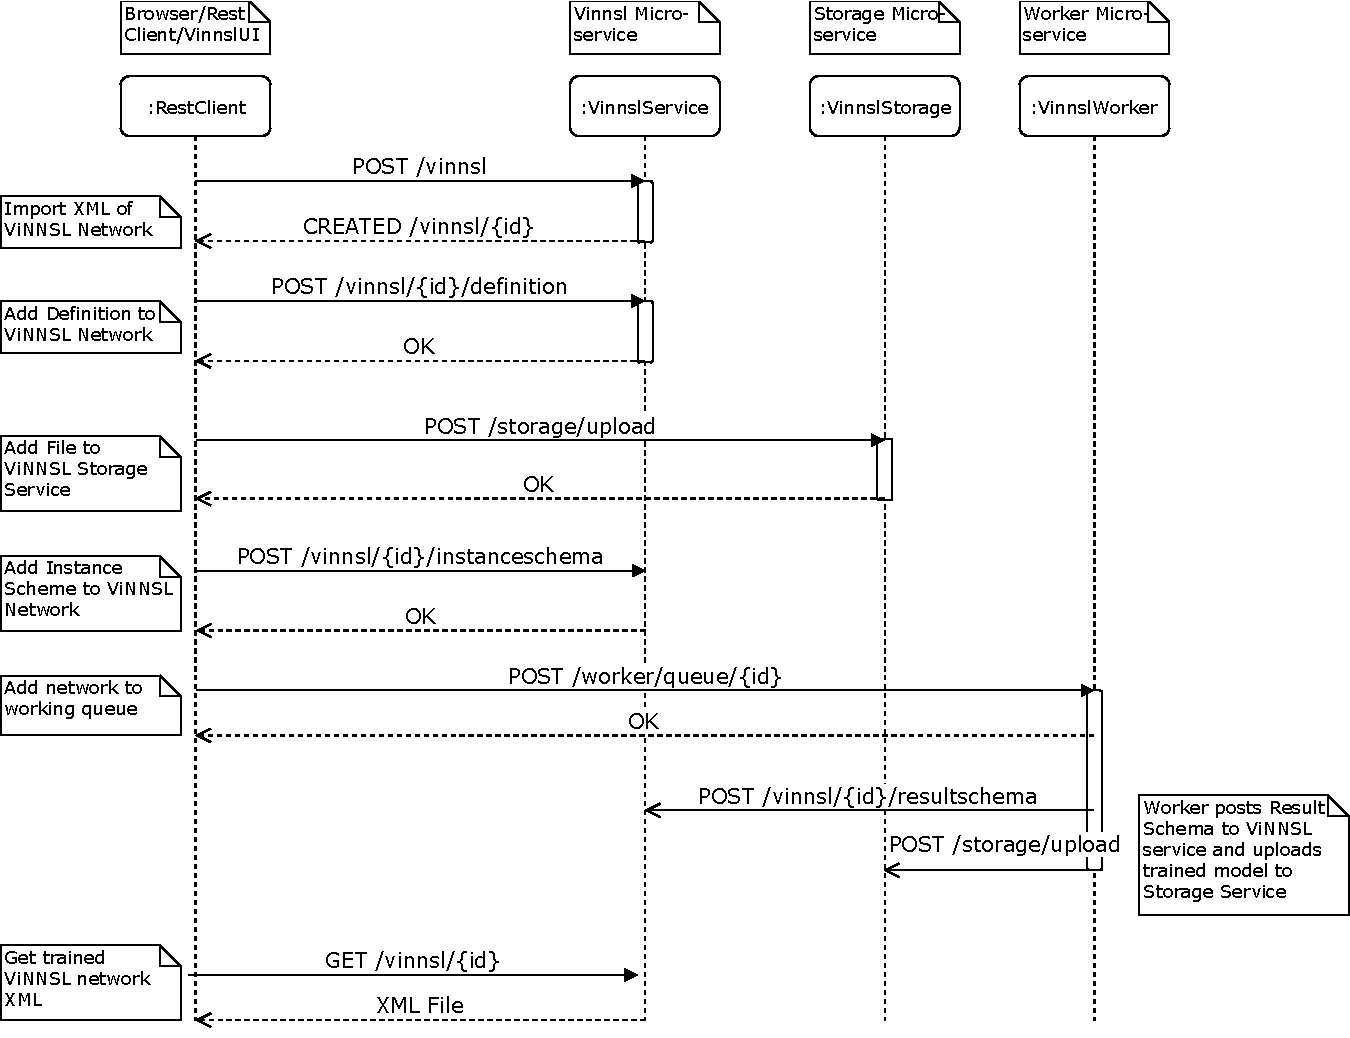
\includegraphics[width=15.00000cm]{images/training_sequence}
\caption{Training Sequence Diagram \label{img.training_sequence}}
\end{figure}

\section{Data Model Design}\label{data-model-design}

\subsection{vinnsl-service}\label{vinnsl-service}

All neural network data managed by the \texttt{vinnsl-service} is stored
in a documented-oriented database. The saved documents will internally
be mapped to Java Classes. The main object is \texttt{vinnsl}.

\texttt{vinnsl} is the primary object owning the \texttt{\_id} field
that is unique. The \texttt{nncloud} property stores the status of the
network and the representation of the transformed \emph{Deeplearning4J}
network. \texttt{description}, \texttt{definition}, \texttt{instance},
\texttt{training} and \texttt{result} represent the ViNNSL 2.0 Schema,
generated from the provided XML Schema Definition files. See
\cite{kopica_2015} to get a listing and description on all provided
properties of ViNNSL 2.0.

Figure \ref{img.db_schema} shows the data schema.

\begin{figure}
\centering
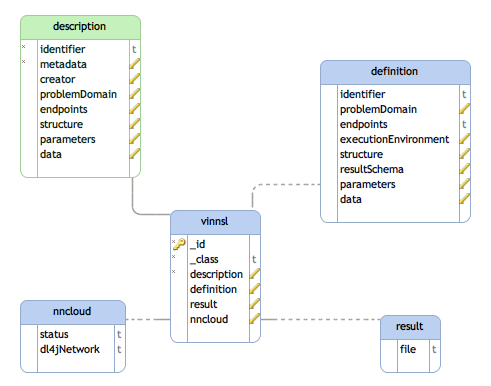
\includegraphics[width=15.00000cm]{images/db_schema}
\caption{NoSQL Data Model \label{img.db_schema}}
\end{figure}

\subsection{storage-service}\label{storage-service}

The \texttt{storage-service} stores binary files and their metadata,
either directly in the file system or inside a database. Each file needs
to have a unique id, a filename, a content type and an upload date.

\begin{longtable}[]{@{}ll@{}}
\toprule
Attribute field & Description\tabularnewline
\midrule
\endhead
id & a unique file id that can be referred to (f.ex in
\texttt{vinnsl-service})\tabularnewline
filename & the original filename when uploaded\tabularnewline
content type & the MIME type standardized in RFC 6838 (f.ex
text/plain)\tabularnewline
upload date & date and time of original upload\tabularnewline
metadata & a field for arbitrary additional information\tabularnewline
\bottomrule
\end{longtable}

Example of stored file:

\begin{verbatim}
{
    "_id" : ObjectId("5ab4e69c8f136a16bf81f093"),
    "filename" : "iris.txt",
    "aliases" : null,
    "chunkSize" : NumberLong(261120),
    "uploadDate" : ISODate("2018-03-23T11:35:56.700Z"),
    "length" : NumberLong(2700),
    "contentType" : "text/plain",
    "md5" : "f0e89bd71f7bb9e584e685aeb178a5aa"
}
\end{verbatim}

\section{Overview Microservices}\label{overview-microservices}

The neural network cloud execution stack consists of four main services
that expose a RESTful API to users and two supporting services in charge
of persisting data. Figure \ref{img.overview_nn_architecture} displays
an overview of the service architecture, including the exposed endpoints
and storage backends.

\begin{figure}
\centering
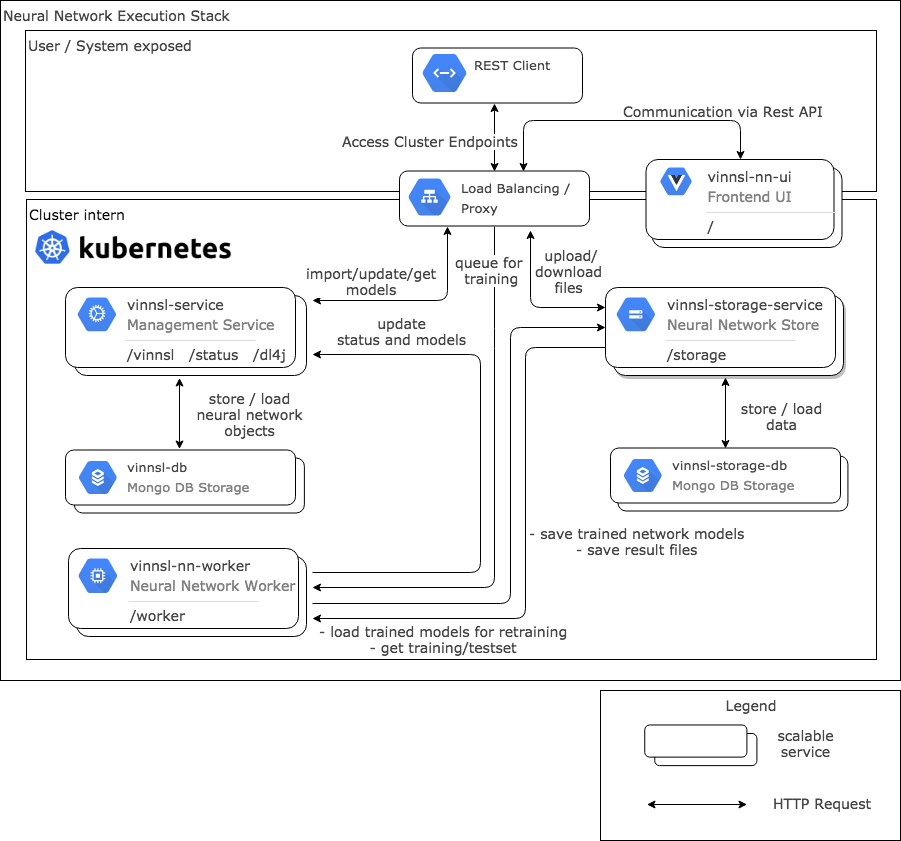
\includegraphics[width=16.50000cm]{images/overview_nn_architecture}
\caption{Architectural Overview of the Neural Network
Stack\label{img.overview_nn_architecture}}
\end{figure}

\subsection{Vinnsl Service
(vinnsl-service)}\label{vinnsl-service-vinnsl-service}

The \texttt{vinnsl-service} is responsible for handling the import,
management and manipulation of neural network objects and it's status.
It maps the CRUD\footnote{Create, Read, Update, Delete} operations to
HTTP methods. A new neural network is created by sending a \texttt{POST}
request to the \texttt{/vinnsl} endpoint containing a ViNNSL Definition
XML as body. Sending a \texttt{GET} request to the \texttt{/vinnsl}
route returns a JSON containing all ViNNSL neural network objects.

The \texttt{vinnsl-service} depends on the \texttt{vinnsl-db} service,
which runs a MongoDB database to store the objects.

\subsection{Worker Service
(vinnsl-nn-worker)}\label{worker-service-vinnsl-nn-worker}

The \texttt{vinnsl-nn-worker} implements a queue management for neural
network training and transforms ViNNSL neural network models into
\emph{Deeplearning4J} models. It provides a wrapper of the
\emph{Deeplearning4J} platform, that handles the training or evaluation
of the network.

\subsection{Storage Service
(vinnsl-storage-service)}\label{storage-service-vinnsl-storage-service}

Binary files, like trained network models, images or csv files are
essential in the pocess of creating and training neural networks. File
management is handled by the \texttt{vinnsl-storage-service}.

\subsection{Frontend UI (vinnsl-nn-ui)}\label{frontend-ui-vinnsl-nn-ui}

The Frontend UI is a web application that gives a brief overview of all
neural network models, their training status and linked files.

\section{User Interface Design}\label{user-interface-design}

Based on the mockup in section \ref{mockup}, a user interface design has
been created, that will later be implemented as a web application.
Buttons to import, delete a neural network and to refresh the user
interface have been added to the design.

Figure \ref{vinnsl-ui-design} shows the user interface design for the
frontend web service.

\begin{figure}
\centering
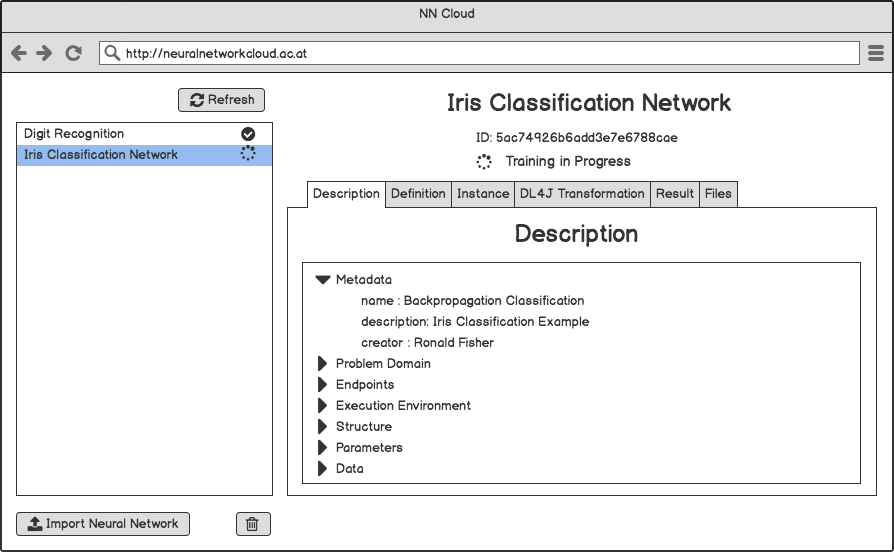
\includegraphics[width=17.00000cm]{images/vinnsl-ui-design}
\caption{User Interface Design for vinnsl-nn-ui
\label{vinnsl-ui-design}}
\end{figure}

\section{Service Discovery and Load
Balancing}\label{service-discovery-and-load-balancing}

\emph{Service Discovery} is the process of finding out how to connect to
a specific service. This applies within the cluster, which is typically
firewalled from the internet. As Kubernetes allows services to be
scaled, there is also a logic that knows and decides how network traffic
is routed. This is called \emph{Load Balancing}. Figure
\ref{img.service-discovery} shows an overview of the microservices,
their endpoint URL and the domain name service. External access to
specific services is managed by \emph{Ingress}.

\subsection{Kubernetes DNS-based Service
Discovery}\label{kubernetes-dns-based-service-discovery}

\texttt{kube-dns} is the Kubernetes add-on that starts a pod with a DNS
service and configures the kubelets to resolve DNS names over this
service. It listens on port 53, the standard DNS port. Services in a
cluster are assigned a DNS A record derived from their service metadata
name specified in the \emph{ServiceSpec}. \cite{kub-dns-spec}

The following code snippet is an extract of the \emph{ServiceSpec} for
the \texttt{vinnsl-service} defining the metadata name:

\begin{verbatim}
{
  "kind": "Service",
  "apiVersion": "v1",
  "metadata": {
    "name": "vinnsl-service",
    ...
  }
}
\end{verbatim}

\subsubsection{Structure of the
Hostname}\label{structure-of-the-hostname}

The full hostname record is composed of the zone, kind, namespace of the
cluster and the metadata name of the service.

\begin{longtable}[]{@{}ll@{}}
\toprule
Name & Description\tabularnewline
\midrule
\endhead
zone & the cluster domain (default using minikube:
\emph{cluster.local})\tabularnewline
kind & kind of pod (default for services: \emph{svc})\tabularnewline
ns & namespace (default using minikube: \emph{default})\tabularnewline
hostname & hostname from service metadata name\tabularnewline
\bottomrule
\end{longtable}

\paragraph{Example}\label{example}

The vinnsl-service running on a local minikube cluster gets the
following DNS record name:
\texttt{vinnsl-service.default.svc.cluster.local}.

\subsubsection{Service Discovery}\label{service-discovery}

Using the Kubernetes DNS service a microservice instance (kubelet) can
now lookup other services by using DNS Queries.

\paragraph{Example}\label{example-1}

For example the tool \texttt{nslookup} can query the DNS service for the
IP address of the \texttt{vinnsl-service} within the cluster.

\begin{verbatim}
/ # nslookup vinnsl-service
Server:    10.96.0.10
Address 1: 10.96.0.10 kube-dns.kube-system.svc.cluster.local

Name:      vinnsl-service
Address 1: 10.102.84.122 vinnsl-service.default.svc.cluster.local
\end{verbatim}

In this example the service is reachable at the IP address
\emph{10.102.84.122}.

\begin{figure}
\centering
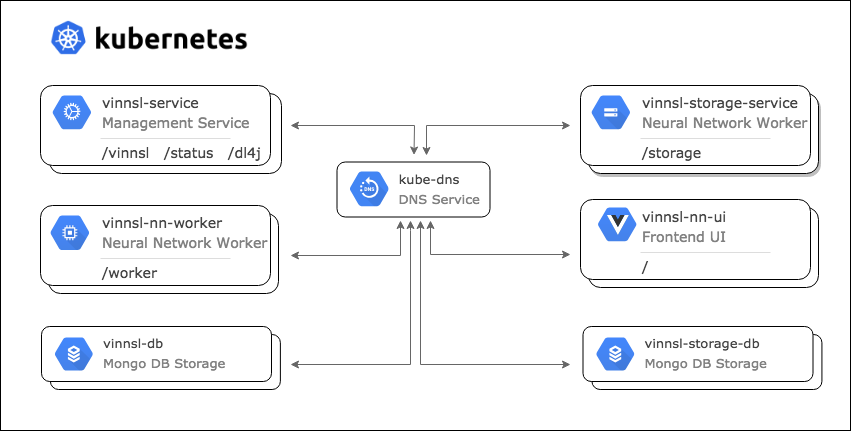
\includegraphics[width=15.00000cm]{images/overview_main_services}
\caption{Service Discovery with kube-dns \label{img.service-discovery}}
\end{figure}

\subsubsection{External Access and Load
Balancing}\label{external-access-and-load-balancing}

External Access from outside the cluster to specific services is managed
and provided through the \emph{Ingress} API object. The associated
implementation is called \emph{Ingress controller} and is obligatory.
Currently there are two official implementations: \texttt{ingress-gce}
and \texttt{ingress-nginx}. \cite{kub-ingress}

\emph{Minikube} runs the \texttt{ingress-nginx} implementation as
default and also provides basic load balancing by configuring a
\texttt{nginx} \footnote{https://archive.ics.uci.edu/ml/datasets/iris}
web server. Kubernetes configures \texttt{nginx} to use the
\emph{least-connected} load balancing mechanism, which means that the
\emph{next request is assigned to the server with the least number of
active connections} \cite{nginx-loadbal}.

\section{Neural Network Objects
State}\label{neural-network-objects-state}

The state of neural network objects is saved in the \texttt{NnCloud}
object. When the object is instantiated the default value is
\texttt{CREATED}. When the network is queued, the worker service gathers
all the necessary data from the vinnsl and vinnsl storage service and
changes the state the \texttt{QUEUED}. During the network training, the
worker changes the state to \texttt{INPROGRESS}. As soon as the training
is finished, the worker service uploads the results and updated network
state to the storage service and subsequently changes the state to
\texttt{FINISHED}. Trained networks can be queued for retraining: in
that case the state returns to \texttt{QUEUED}. If errors occur during
the training process the state will be set to \texttt{ERROR}.

Figure \ref{nn-states} visualizes the state changes in a state machine.

\begin{figure}
\centering
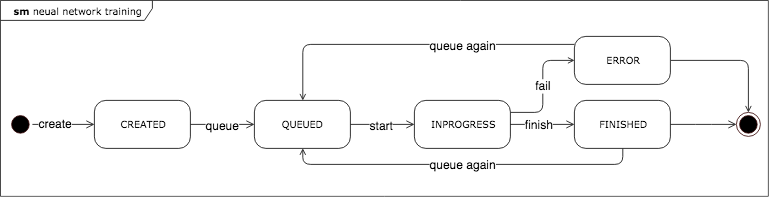
\includegraphics[width=15.00000cm]{images/nn-states}
\caption{State Machine of a Neural Network \label{nn-states}}
\end{figure}

\chapter{Prototype Implementation}\label{prototype-implementation}

Following the specification, this section showcases an implementation of
a prototype using microservices glued together by \emph{Kubernetes}.
This represents the execution stack for neural networks. Backend
components are realized with \emph{Java} and the \emph{Spring Boot}
framework and expose a RESTful API. The processing and training of
neural networks is done by the \emph{Deeplearning4J} framework. Database
and file storage are powered by \emph{MongoDB}. The frontend service is
implemented using \emph{Vue.js} and the \emph{Twitter Bootstrap} UI
framework, visualizing and consuming backend services.

\section{Source Code}\label{source-code-1}

The source code of the implemented microservices is released on
\emph{GitHub}. The following table gives an overview of available
services and their corresponding repository.

\begin{longtable}[]{@{}ll@{}}
\toprule
\begin{minipage}[b]{0.29\columnwidth}\raggedright\strut
Name\strut
\end{minipage} & \begin{minipage}[b]{0.65\columnwidth}\raggedright\strut
Repository Link\strut
\end{minipage}\tabularnewline
\midrule
\endhead
\begin{minipage}[t]{0.29\columnwidth}\raggedright\strut
vinnsl-service\strut
\end{minipage} & \begin{minipage}[t]{0.65\columnwidth}\raggedright\strut
https://github.com/a00908270/vinnsl-service\strut
\end{minipage}\tabularnewline
\begin{minipage}[t]{0.29\columnwidth}\raggedright\strut
vinnsl-nn-ui\strut
\end{minipage} & \begin{minipage}[t]{0.65\columnwidth}\raggedright\strut
https://github.com/a00908270/vinnsl-nn-ui\strut
\end{minipage}\tabularnewline
\begin{minipage}[t]{0.29\columnwidth}\raggedright\strut
vinnsl-storage-service\strut
\end{minipage} & \begin{minipage}[t]{0.65\columnwidth}\raggedright\strut
https://github.com/a00908270/vinnsl-storage-service\strut
\end{minipage}\tabularnewline
\begin{minipage}[t]{0.29\columnwidth}\raggedright\strut
vinnsl-nn-worker\strut
\end{minipage} & \begin{minipage}[t]{0.65\columnwidth}\raggedright\strut
https://github.com/a00908270/vinnsl-nn-worker\strut
\end{minipage}\tabularnewline
\bottomrule
\end{longtable}

The \emph{ViNNSL} XSD schema specified in \cite{kopica_2015} including
(generated) examples is released on GitHub with permission from
Dipl.-Ing. Thomas Kopica. JAXB class generation of the XML files is
already included in the release with the intention of making it easier
to include \emph{ViNNSL} into new services.

\begin{longtable}[]{@{}ll@{}}
\toprule
Name & Repository Link\tabularnewline
\midrule
\endhead
vinnsl-schema &
https://github.com/a00908270/vinnsl-schema\tabularnewline
\bottomrule
\end{longtable}

\section{Releases}\label{releases}

Docker Contrainers ready for deployment in a \emph{Kubernetes} cluster
are released on \emph{DockerHub}. The following table references the
released repositories.

\begin{longtable}[]{@{}ll@{}}
\toprule
\begin{minipage}[b]{0.26\columnwidth}\raggedright\strut
Name\strut
\end{minipage} & \begin{minipage}[b]{0.68\columnwidth}\raggedright\strut
Repository Link\strut
\end{minipage}\tabularnewline
\midrule
\endhead
\begin{minipage}[t]{0.26\columnwidth}\raggedright\strut
vinnsl-service\strut
\end{minipage} & \begin{minipage}[t]{0.68\columnwidth}\raggedright\strut
https://hub.docker.com/r/a00908270/vinnsl-service/\strut
\end{minipage}\tabularnewline
\begin{minipage}[t]{0.26\columnwidth}\raggedright\strut
vinnsl-nn-ui\strut
\end{minipage} & \begin{minipage}[t]{0.68\columnwidth}\raggedright\strut
https://hub.docker.com/r/a00908270/vinnsl-nn-ui/\strut
\end{minipage}\tabularnewline
\begin{minipage}[t]{0.26\columnwidth}\raggedright\strut
vinnsl-storage-service\strut
\end{minipage} & \begin{minipage}[t]{0.68\columnwidth}\raggedright\strut
https://hub.docker.com/r/a00908270/vinnsl-storage-service/\strut
\end{minipage}\tabularnewline
\begin{minipage}[t]{0.26\columnwidth}\raggedright\strut
vinnsl-nn-worker\strut
\end{minipage} & \begin{minipage}[t]{0.68\columnwidth}\raggedright\strut
https://hub.docker.com/r/a00908270/vinnsl-nn-worker/\strut
\end{minipage}\tabularnewline
\bottomrule
\end{longtable}

\section{Framework Dependencies}\label{framework-dependencies}

All services are written in \emph{Java} and build using the \emph{Apache
Maven} build automation and dependency management tool.

\subsection{Spring}\label{spring}

\emph{Spring} is a \emph{Java} framework consisting of many modules,
most importantly this project uses its feature so set up
\texttt{RestController} instances that listen on specified endpoints.

\paragraph{Used in following
services:}\label{used-in-following-services}

\texttt{vinnsl-service}, \texttt{vinnsl-nn-ui},
\texttt{vinnsl-storage-service}, \texttt{vinnsl-nn-worker}

\subsubsection{Spring Boot}\label{spring-boot}

\emph{Spring Boot} is an extension to the framework that allows
\emph{Java} applications to run stand-alone by embedding a web server
directly into the application. \cite{spring-boot}

\paragraph{Used in following
services:}\label{used-in-following-services-1}

\texttt{vinnsl-service}, \texttt{vinnsl-nn-ui},
\texttt{vinnsl-storage-service}, \texttt{vinnsl-nn-worker}

\subsubsection{Spring Data MongoDB}\label{spring-data-mongodb}

\emph{Spring Data} provides an abstracted database access layer to
MongoDB in form of a POJO (Plain Old Java Object). \cite{spring-data}

\paragraph{Used in following
services:}\label{used-in-following-services-2}

\texttt{vinnsl-service}, \texttt{vinnsl-storage-service}

\subsection{Swagger}\label{swagger}

\emph{Swagger} is used to generate a live documentation of all web
service endpoints in this project and allows to try out requests
directly in the user interface.

\paragraph{Used in following
services:}\label{used-in-following-services-3}

\texttt{vinnsl-service}, \texttt{vinnsl-storage-service},
\texttt{vinnsl-nn-worker}

\subsection{Fabric8}\label{fabric8}

\emph{Fabric8} packs the generated executables from the build process
into a \emph{Docker} container that can run in a \emph{Kubernetes}
cluster. The process is described in detail in section TODO

\paragraph{Used in following
services:}\label{used-in-following-services-4}

\texttt{vinnsl-service}, \texttt{vinnsl-nn-ui},
\texttt{vinnsl-storage-service}, \texttt{vinnsl-nn-worker}

\subsection{Deeplearning4J}\label{deeplearning4j-1}

\emph{Deeplearning4J} is used by the worker service to train and
evaluate neural networks.

A detailed introduction to Deeplearning4J can be found in Section
\ref{deeplearning4j}.

\paragraph{Used in following
services:}\label{used-in-following-services-5}

\texttt{vinnsl-nn-worker}

\section{Security}\label{security}

\emph{Ingress} supports HTTPS encrypted connections. Authentication or
restrictions are not implemented in the prototype.

\section{User Interface}\label{user-interface-1}

\subsection{vinnsl-nn-ui (Frontend UI)}\label{vinnsl-nn-ui-frontend-ui}

The \texttt{vinnsl-nn-ui} is a single page application (SPA) that
displays all neural networks and their details in a web based frontend.
Figure \ref{img.vinnsl-nn-ui} shows a screenshot of the user interface.

\begin{figure}
\centering
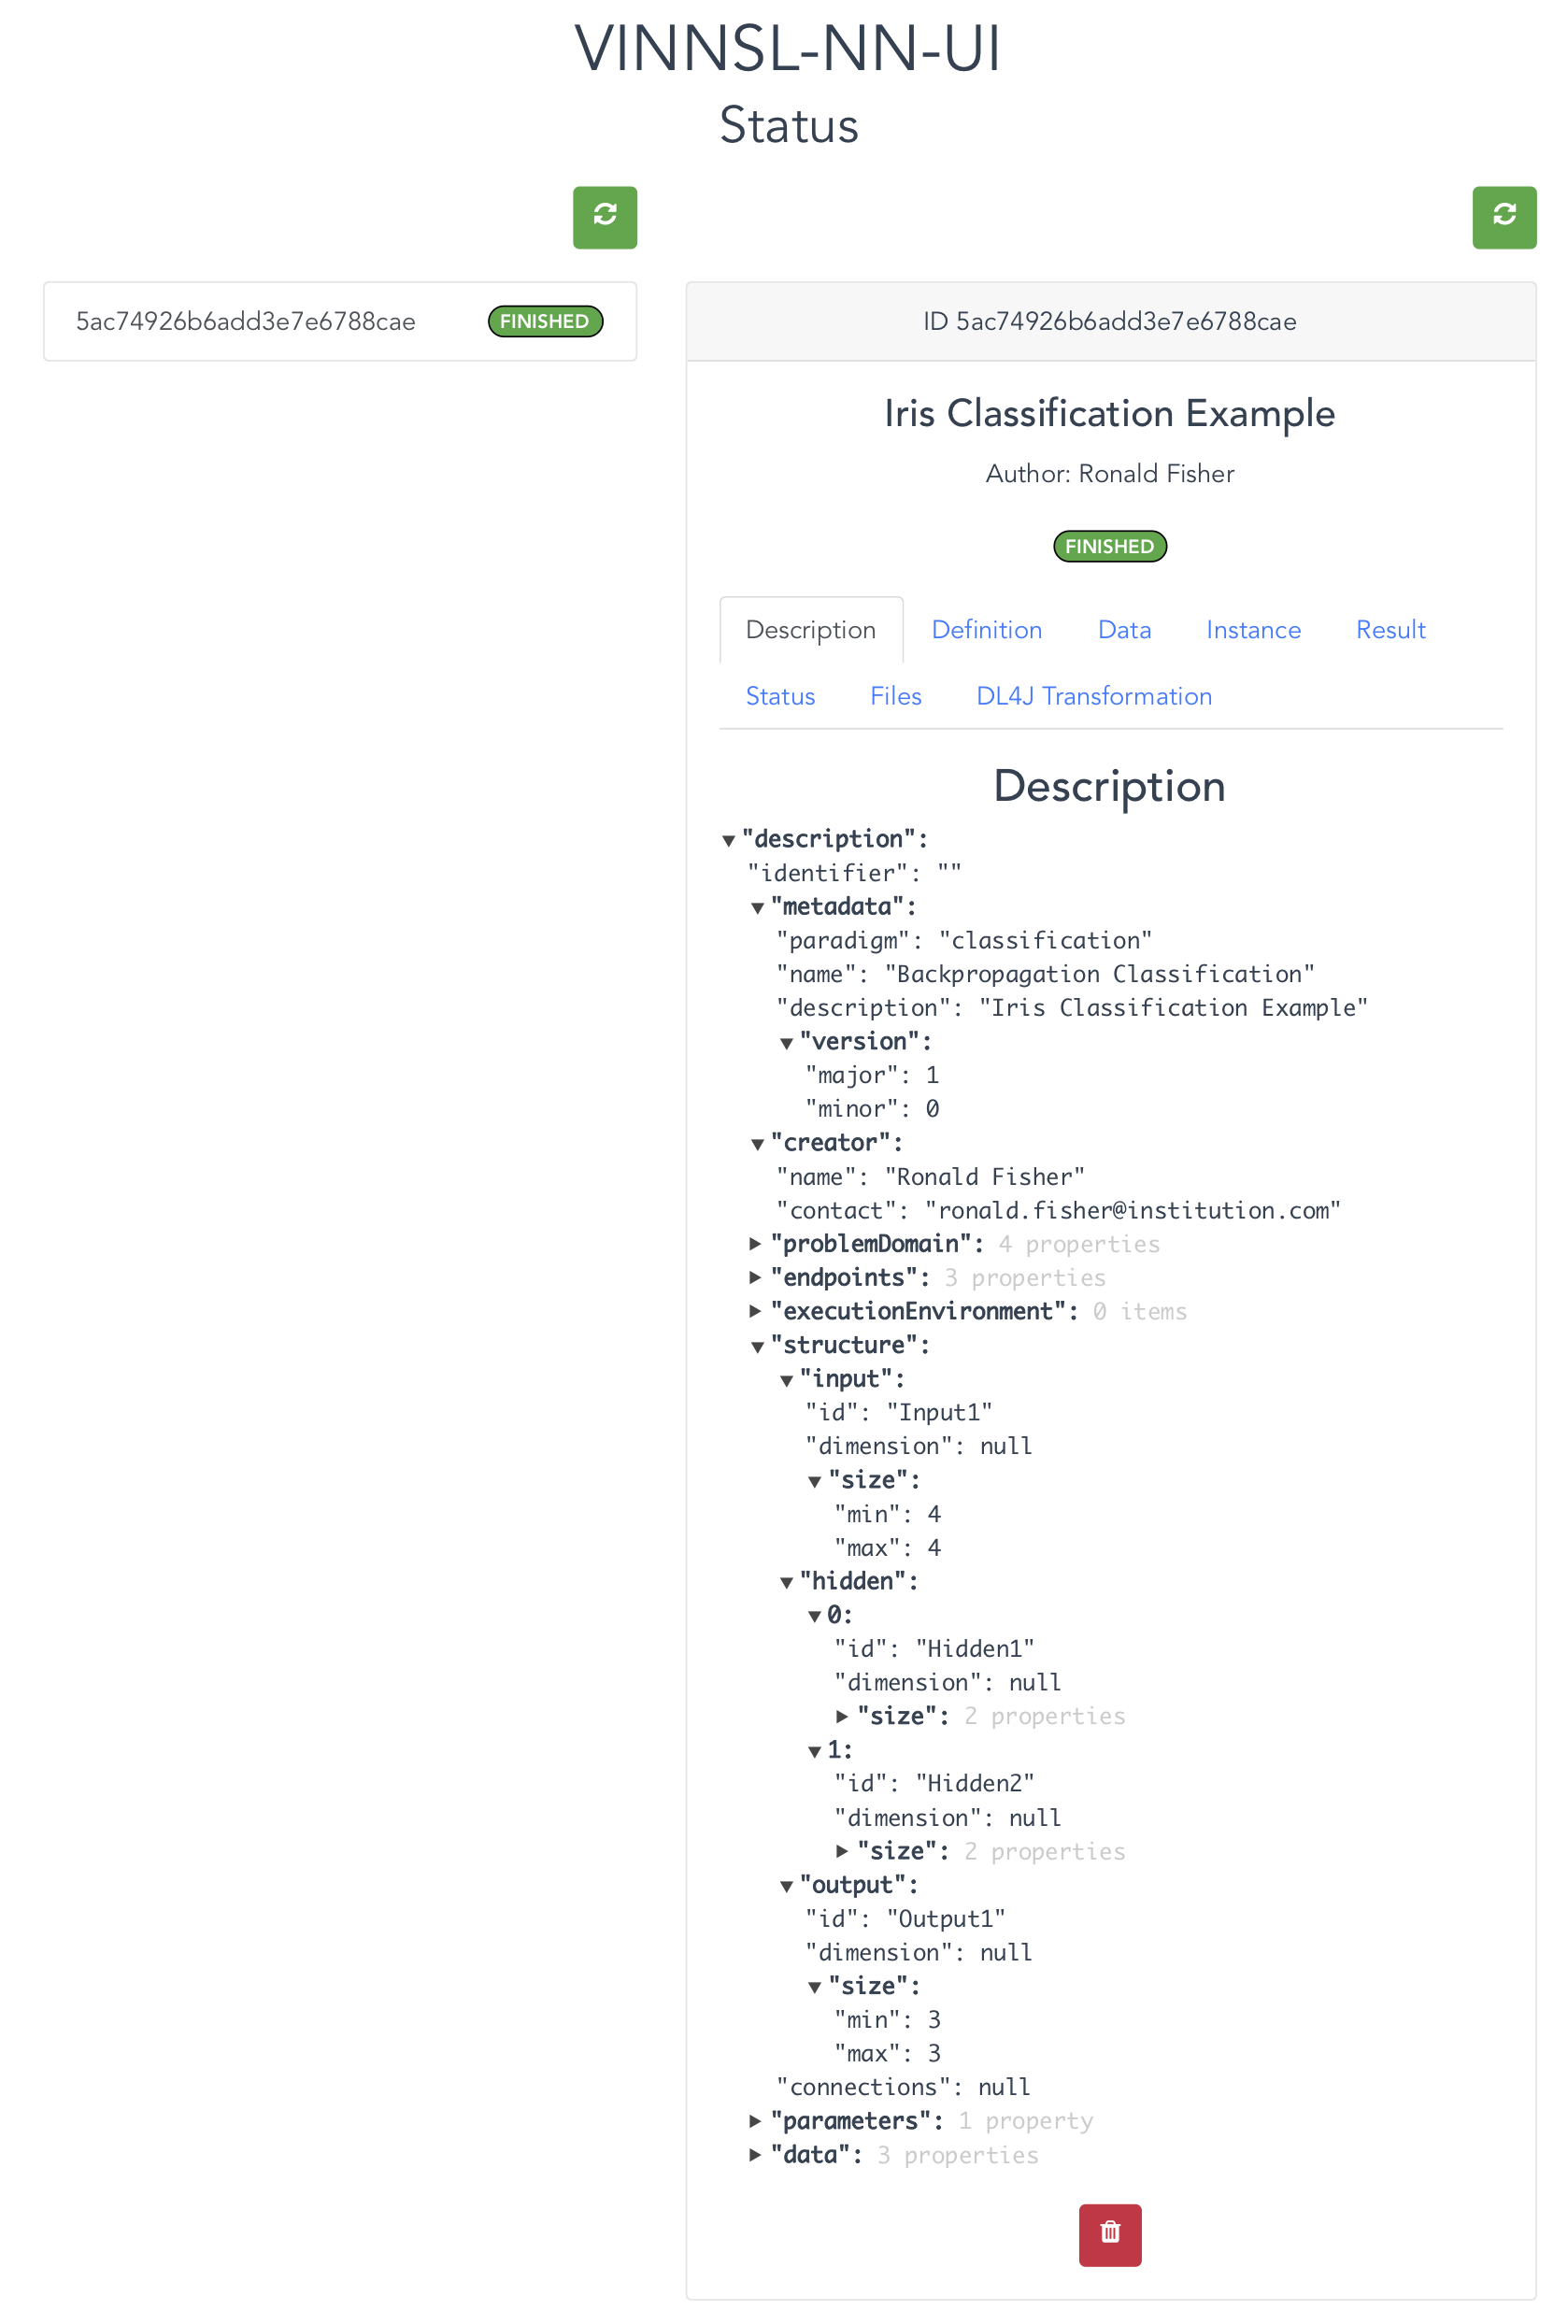
\includegraphics[width=15.00000cm]{images/VINNSL-NN-UI}
\caption{User Interface of Prototype \label{img.vinnsl-nn-ui}}
\end{figure}

\subsubsection{Architecture}\label{architecture}

The web application is a Javascript based frontend using the
\emph{Vue.js} and \emph{Twitter Bootstrap} framework. The single main
controller called \texttt{VinnslUI} provides methods to fetch a list of
neural networks and their status. Additionally it queries for available
files from the storage service and enables to connect them to a neural
network.

\section{Endpoints}\label{endpoints}

The following table gives an overview of the provided RESTful endpoints
provided by different services. They are made available via
\emph{Ingress} outside the \emph{Kubernetes} cluster.

\begin{longtable}[]{@{}ll@{}}
\toprule
Service Name & Exposed Endpoints\tabularnewline
\midrule
\endhead
vinnsl-service & \texttt{/vinnsl}, \texttt{/status},
\texttt{/dl4j}\tabularnewline
vinnsl-nn-ui & \texttt{/}\tabularnewline
vinnsl-storage-service & \texttt{/storage}\tabularnewline
vinnsl-nn-worker & \texttt{/worker}\tabularnewline
\bottomrule
\end{longtable}

\subsection{Additional Endpoints}\label{additional-endpoints}

Additional Endpoints are used internally and not directly exposed
outside the \emph{Kubernetes} cluster. They can be reached by using port
forwarding to directly access the service in the cluster.

\paragraph{/health}\label{health}

The health endpoints returns the status of the application. \texttt{UP}
if the application is running as expected, \texttt{DOWN} if parts of the
application fail (like lost connection to the database).
\emph{Kubernetes} and \emph{Ingress} use this endpoint to detect
disturbances in the application.

\paragraph{/swagger}\label{swagger-1}

The API provided by the services is documented and \emph{Swagger}
provides a web interface to the documentation.

\subsubsection{}\label{section}

\section{Class Diagrams}\label{class-diagrams}

This section features class diagrams of the provided RESTful services.
All of them, as mentioned, are based on Java \emph{Spring Boot} and use
the \emph{Spring Boot Data} layer if connecting to a database.

\subsection{vinnsl-service}\label{vinnsl-service-1}

The \emph{vinnsl service} is the main communication hub that enables
access to the neural network objects and all of its data and provides
interfaces to update it. The service connects to a \emph{MongoDB}
database where all its persisted data is stored via the \emph{Spring
Data} template. Fig. \ref{class_vinnsl-service} shows the class diagram
of the \emph{vinnsl service}.

\subsubsection{VinnslServiceApplication}\label{vinnslserviceapplication}

\texttt{VinnslServiceApplication} is the main class that initializes the
\emph{Spring Boot} configuration and \emph{MongoDB} repository.

\subsubsection{VinnslServiceController}\label{vinnslservicecontroller}

\texttt{VinnslServiceController} is a \emph{Spring}
\texttt{RestController} implementing all Mappings for the endpoint
\texttt{/vinnsl}. All required dependencies on \emph{MongoDB} and are
injected by Spring Boot.

\subsubsection{NnStatusController}\label{nnstatuscontroller}

\texttt{NnStatusController} provides methods to get the current training
status of all or an individual neural network(s). Methods are exposed at
the \texttt{/status} endpoint. Other services, like the \emph{vinnsl
worker service} can also update the status.

\subsubsection{Dl4JServiceController}\label{dl4jservicecontroller}

\texttt{Dl4JServiceController} is a controller that allows manipulation
of the \emph{Deeplearning4J} property of a neural network using the
\texttt{/dl4j} endpoint.

\subsubsection{Vinnsl}\label{vinnsl-1}

The \emph{vinnsl} class is a \emph{POJO}\footnote{Plain Old Java Object}
representation of the \emph{ViNNSL} XML structure and used across
different services.

\subsubsection{NnCloud}\label{nncloud}

The \texttt{NnCloud} class is an extension to \texttt{Vinnsl} used to
store the status and the \emph{Deeplearning4J} representation of a
neural network.

\begin{figure}
\centering
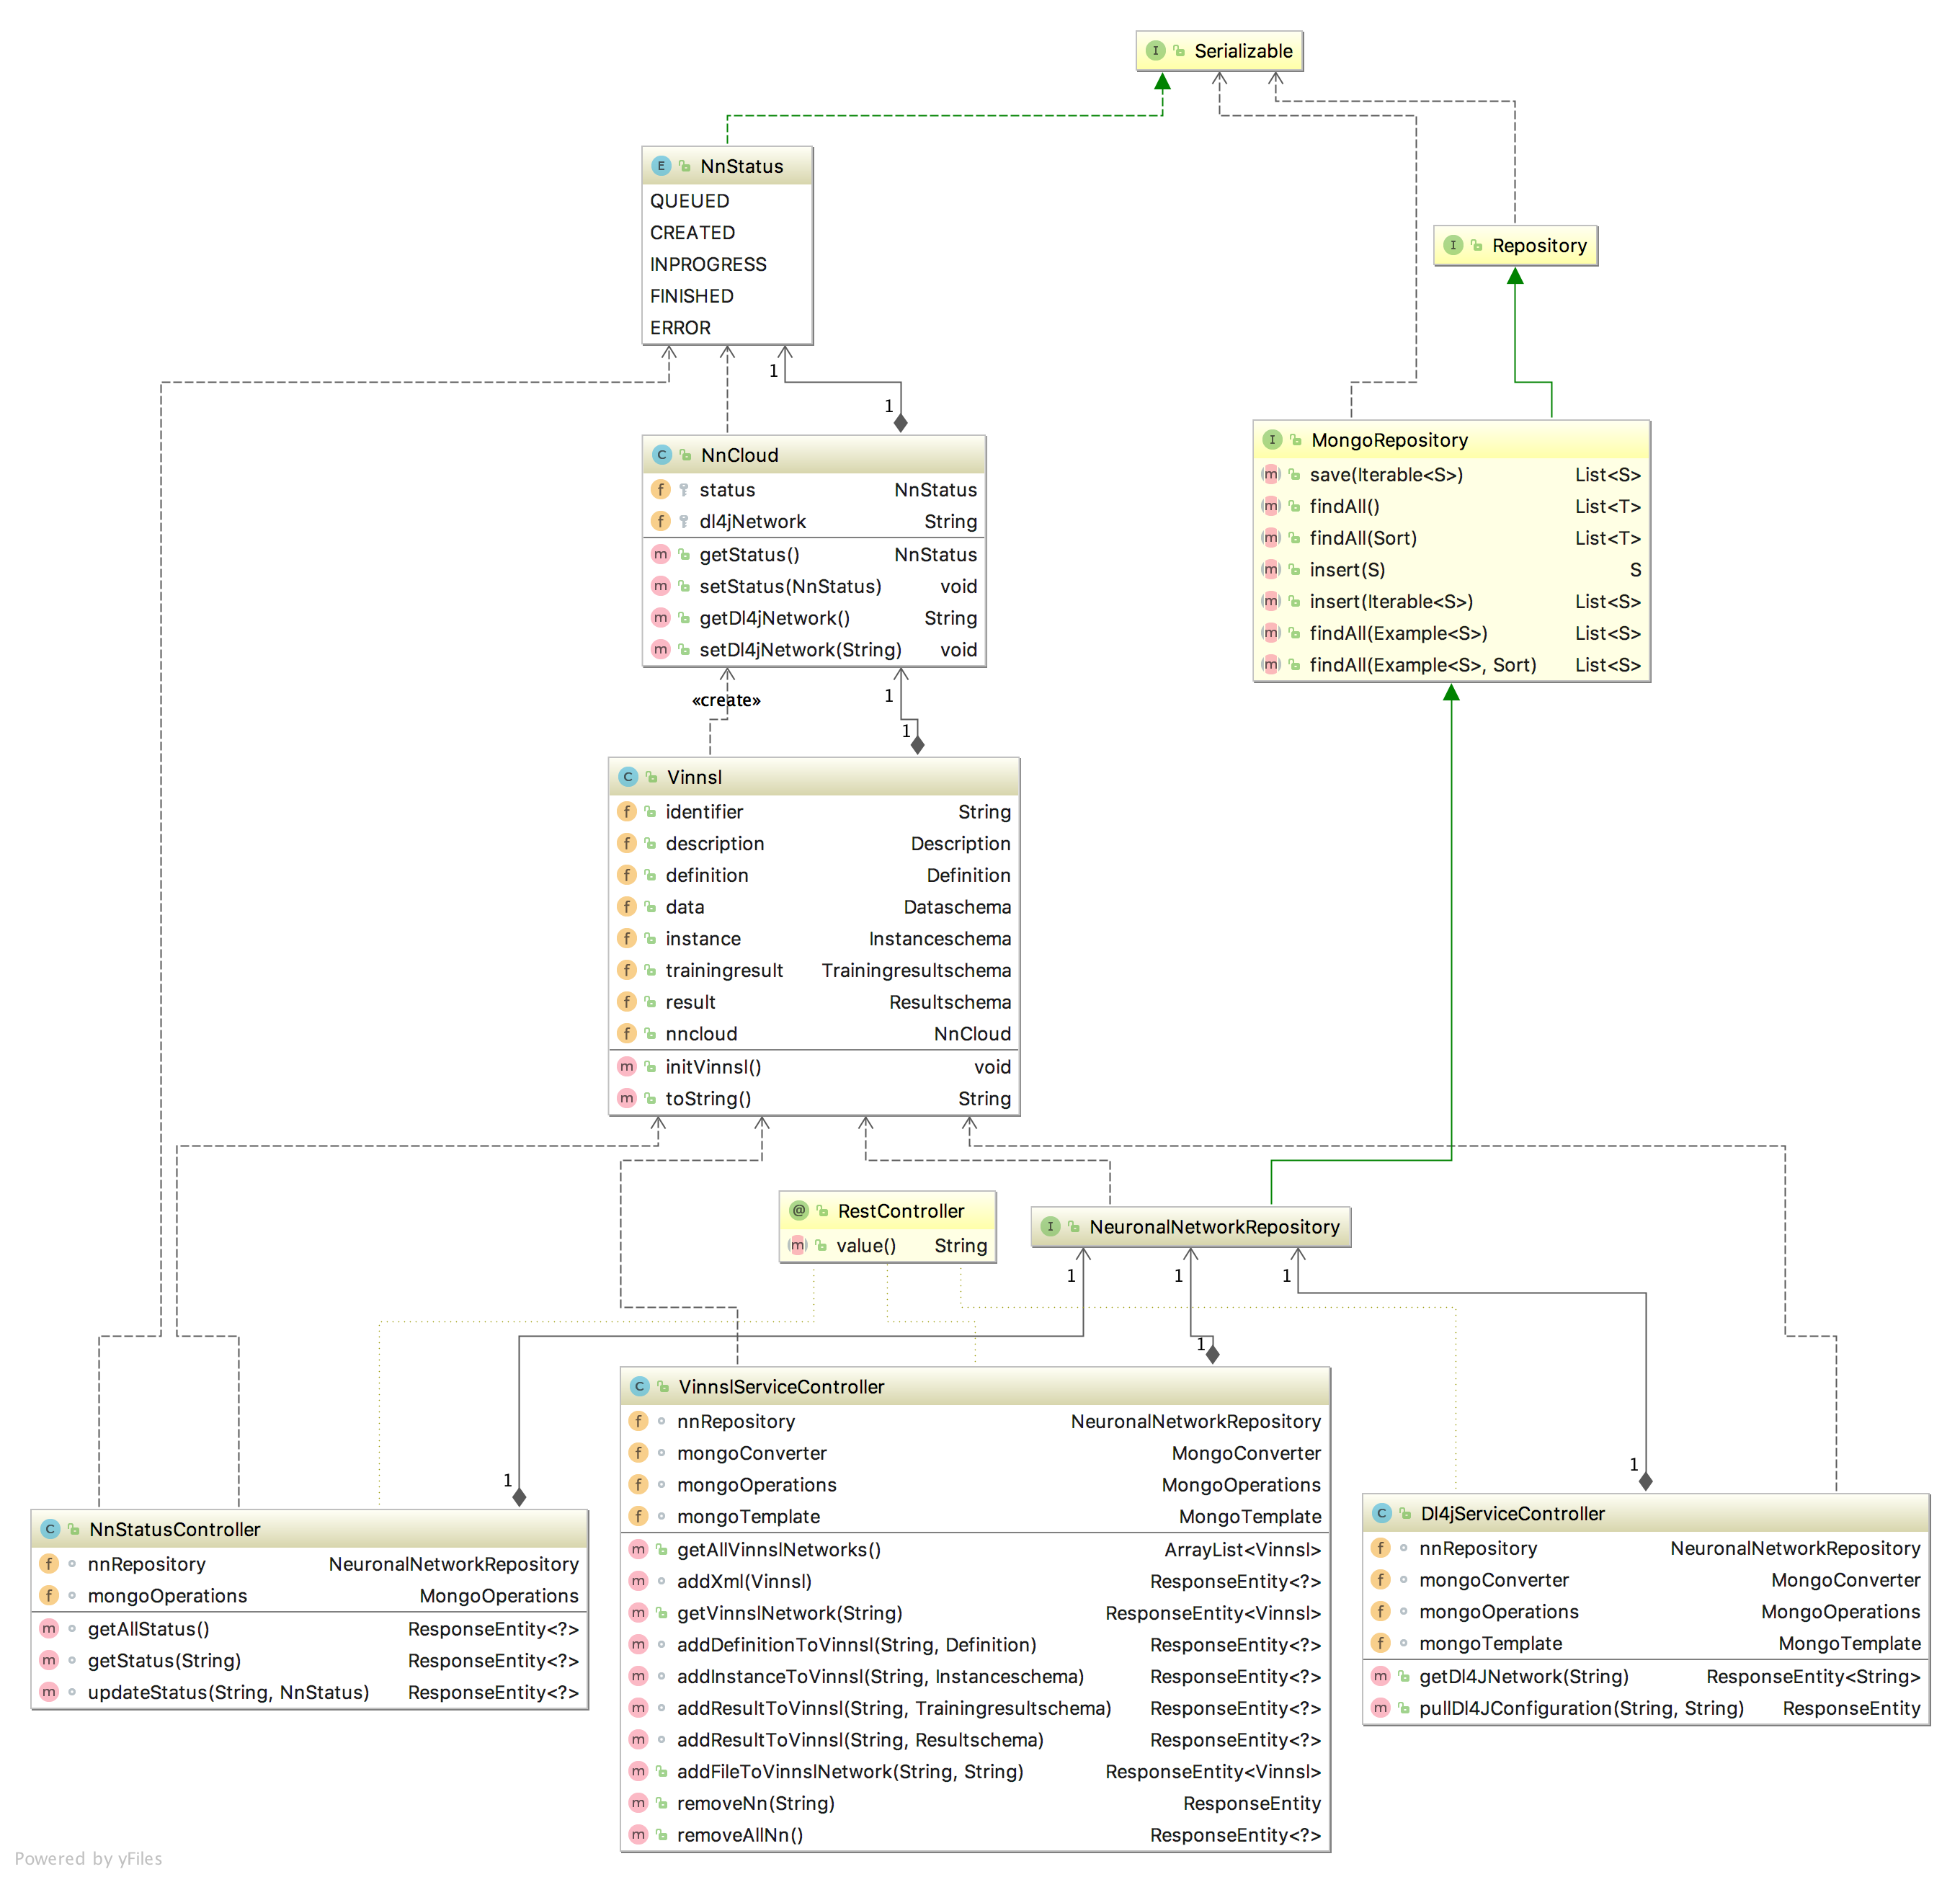
\includegraphics[width=17.00000cm]{images/uml-class-diagram-vinnsl-service}
\caption{Class Diagram of vinnsl-service \label{class_vinnsl-service}}
\end{figure}

\subsection{vinnsl-storage-service}\label{vinnsl-storage-service}

The \emph{vinnsl storage service} is a web service for storing and
retrieving files in a \emph{MongoDB} database. \emph{GridFS}, which
enables to store large data is activated. Figure
\ref{class_vinnsl-storage-service} shows the class diagram.

\subsubsection{VinnslStorageApplication}\label{vinnslstorageapplication}

\texttt{VinnslStorageApplication} is the main class that initializes the
\emph{Spring Boot} configuration and \emph{MongoDB} repository.

\subsubsection{VinnslStorageController}\label{vinnslstoragecontroller}

\texttt{VinnslStorageController} makes retrieving and uploading files
available via the \texttt{/storage} endpoint.

For one there is an HTML form that enables a \texttt{Multipart} file
upload from a browser, which is handled by the
\texttt{handleFileUpload()} method. Secondly instead of directly
uploading a file, a \emph{URL} can be given as parameter via the
\texttt{handleRestFileUploadFromUrl}. The storage service takes care of
downloading and storing the file. The controller uses the \emph{GridFS}
template as an abstraction to the \emph{MongoDB} database.

\begin{figure}
\centering
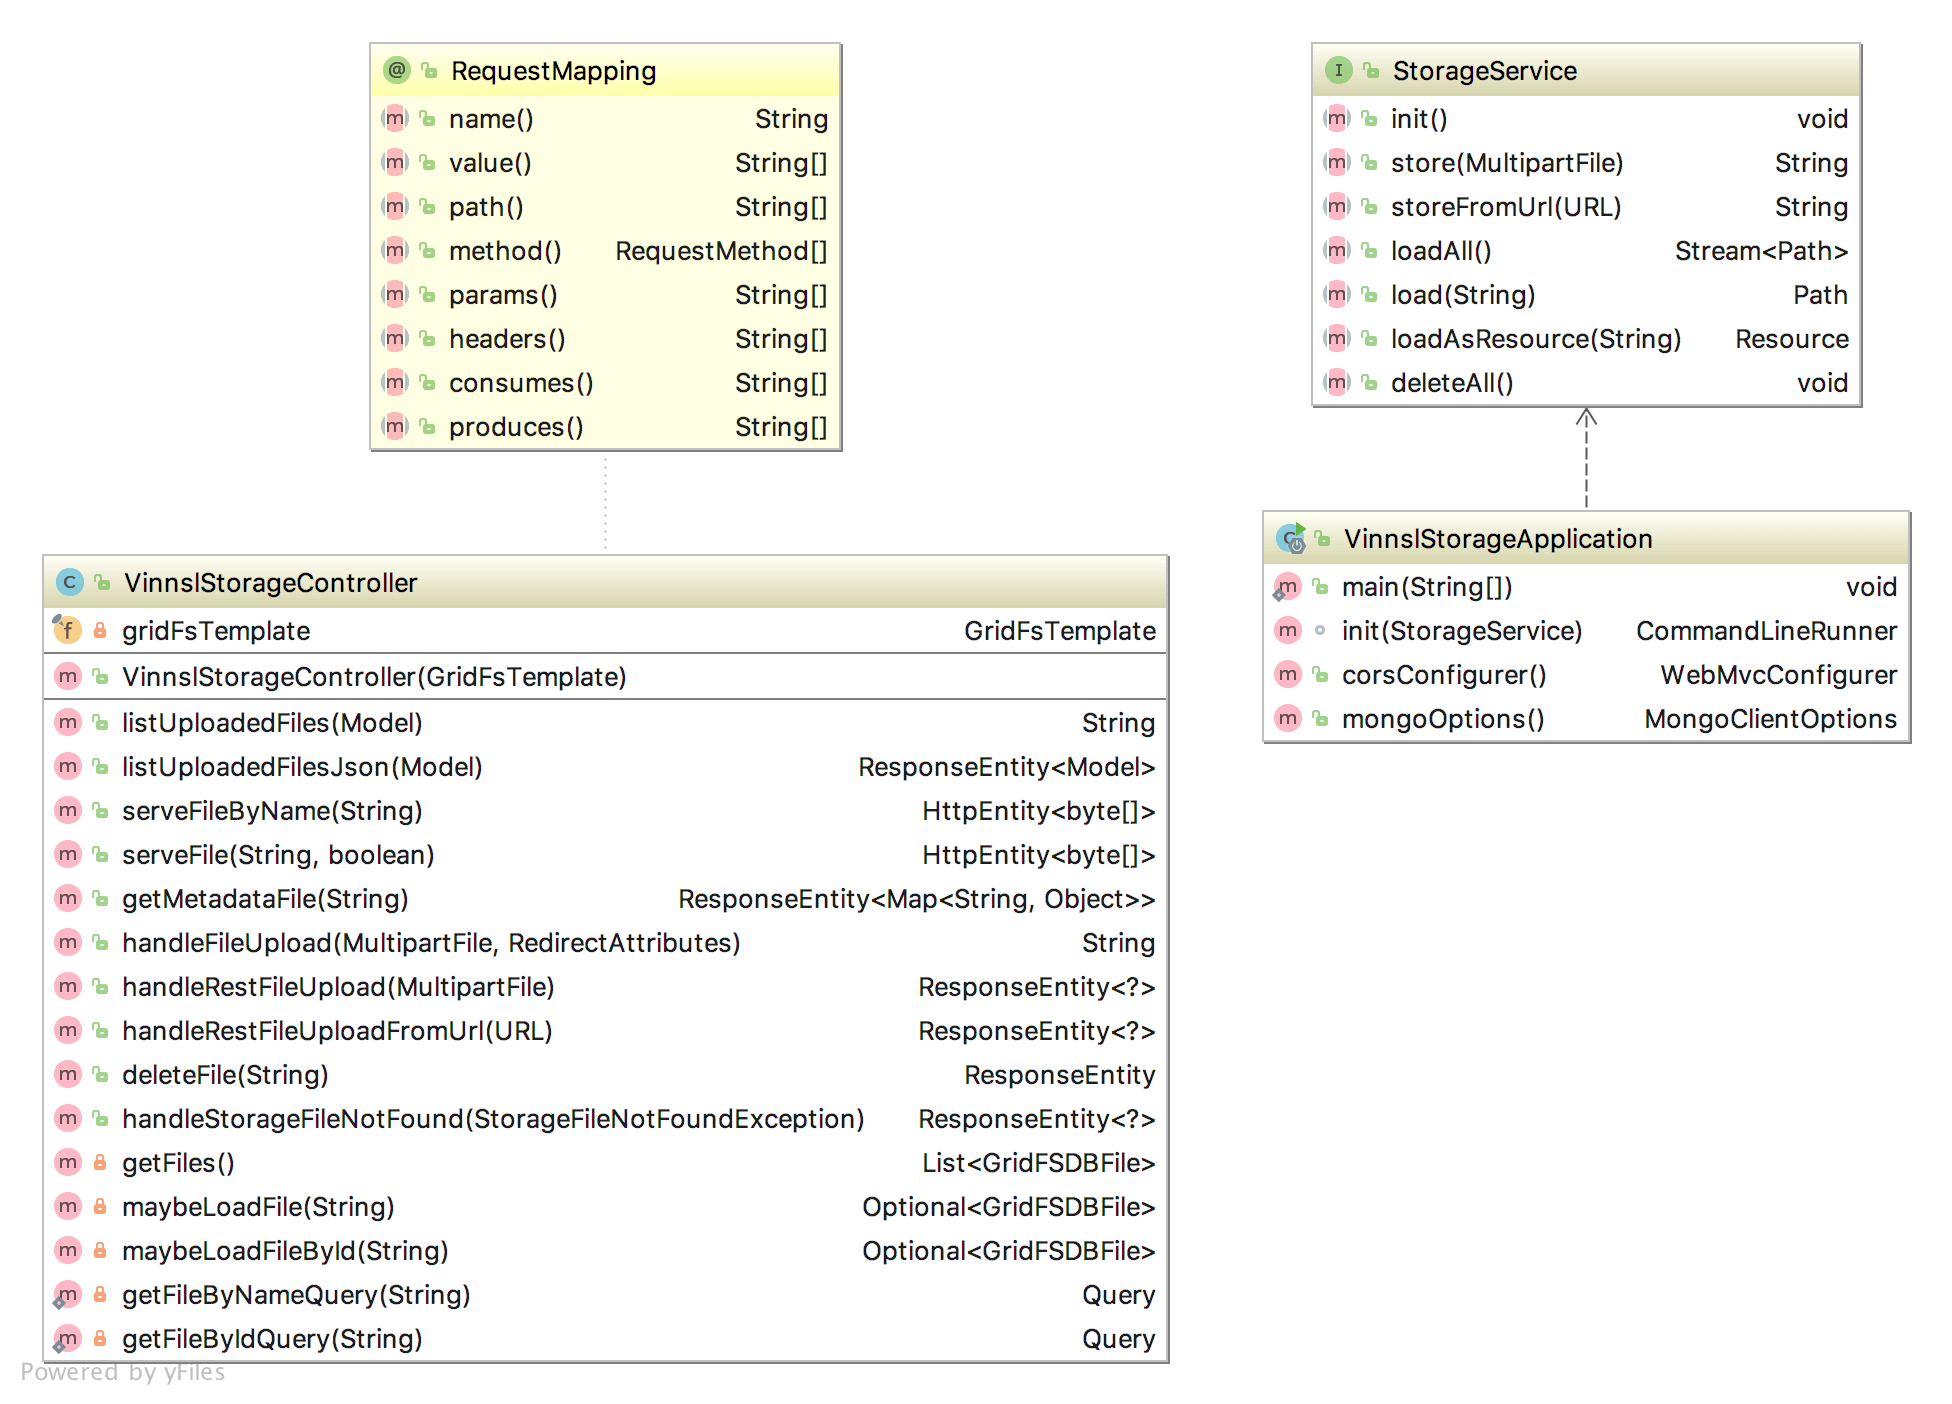
\includegraphics[width=15.00000cm]{images/uml-class-diagram-vinnsl-storage-service}
\caption{Class Diagram of vinnsl-storage-service
\label{class_vinnsl-storage-service}}
\end{figure}

\subsection{vinnsl-worker-service}\label{vinnsl-worker-service}

The \emph{vinnsl worker service} is the component used for training and
evaluating neural networks using the \emph{Deeplearning4J} framework.
Figure \ref{class_vinnsl-worker-service} shows the class diagram.

\subsubsection{MappingUtil /
VinnslDL4JMapperImpl}\label{mappingutil-vinnsldl4jmapperimpl}

The classes \texttt{MappingUtil} and \texttt{VinnslDL4JMapperImpl} are
responsible for mapping a \emph{Vinnsl} to a \emph{DeepLearning4J}
network that can be trained.

The Mappings are done in inner classes of the \texttt{MappingUtil}.
\texttt{VinnslDL4JMapperImpl} initialized the necessary objects and
calls the right methods to perform the mapping.

\subsubsection{Worker Controller}\label{worker-controller}

\texttt{WorkerController} is a \texttt{RestController} that exposes the
\texttt{/worker/queue} endpoint and can be used to schedule neural
networks for training.

\subsubsection{WorkerQueue}\label{workerqueue}

\texttt{WorkerQueue} is the data structure that stores the identifiers
of the queued networks in memory.

\subsubsection{Worker}\label{worker}

The \emph{worker} class checks the \texttt{WorkerQueue} periodically and
if not empty polls the first element. It fetches the associated
\emph{Vinnsl} network from the \emph{vinnsl-service} and hands it over
to the \emph{Dl4JNetworkTrainer}. The service further sets the training
status to \texttt{INPROGRESS}.

\subsubsection{Dl4JNetworkTrainer}\label{dl4jnetworktrainer}

The training is initiated by the \texttt{Worker} class. The
\emph{network trainer} fetches and parses the training data if necessary
(for example \emph{comma separed value} files) and initializes the
\texttt{MappingUtil}. The transformed \emph{Deeplearning4J} model
contains the neural network structure and parameters required for
training and it attached to the \emph{ViNNSL} model.

Next the \emph{Deeplearning4J} \texttt{UI\ Server} is initialized, which
visualizes the training process. Test and training data is split and the
training is started. After the training process is finished, the result
is uploaded to the storage service.

\begin{figure}
\centering
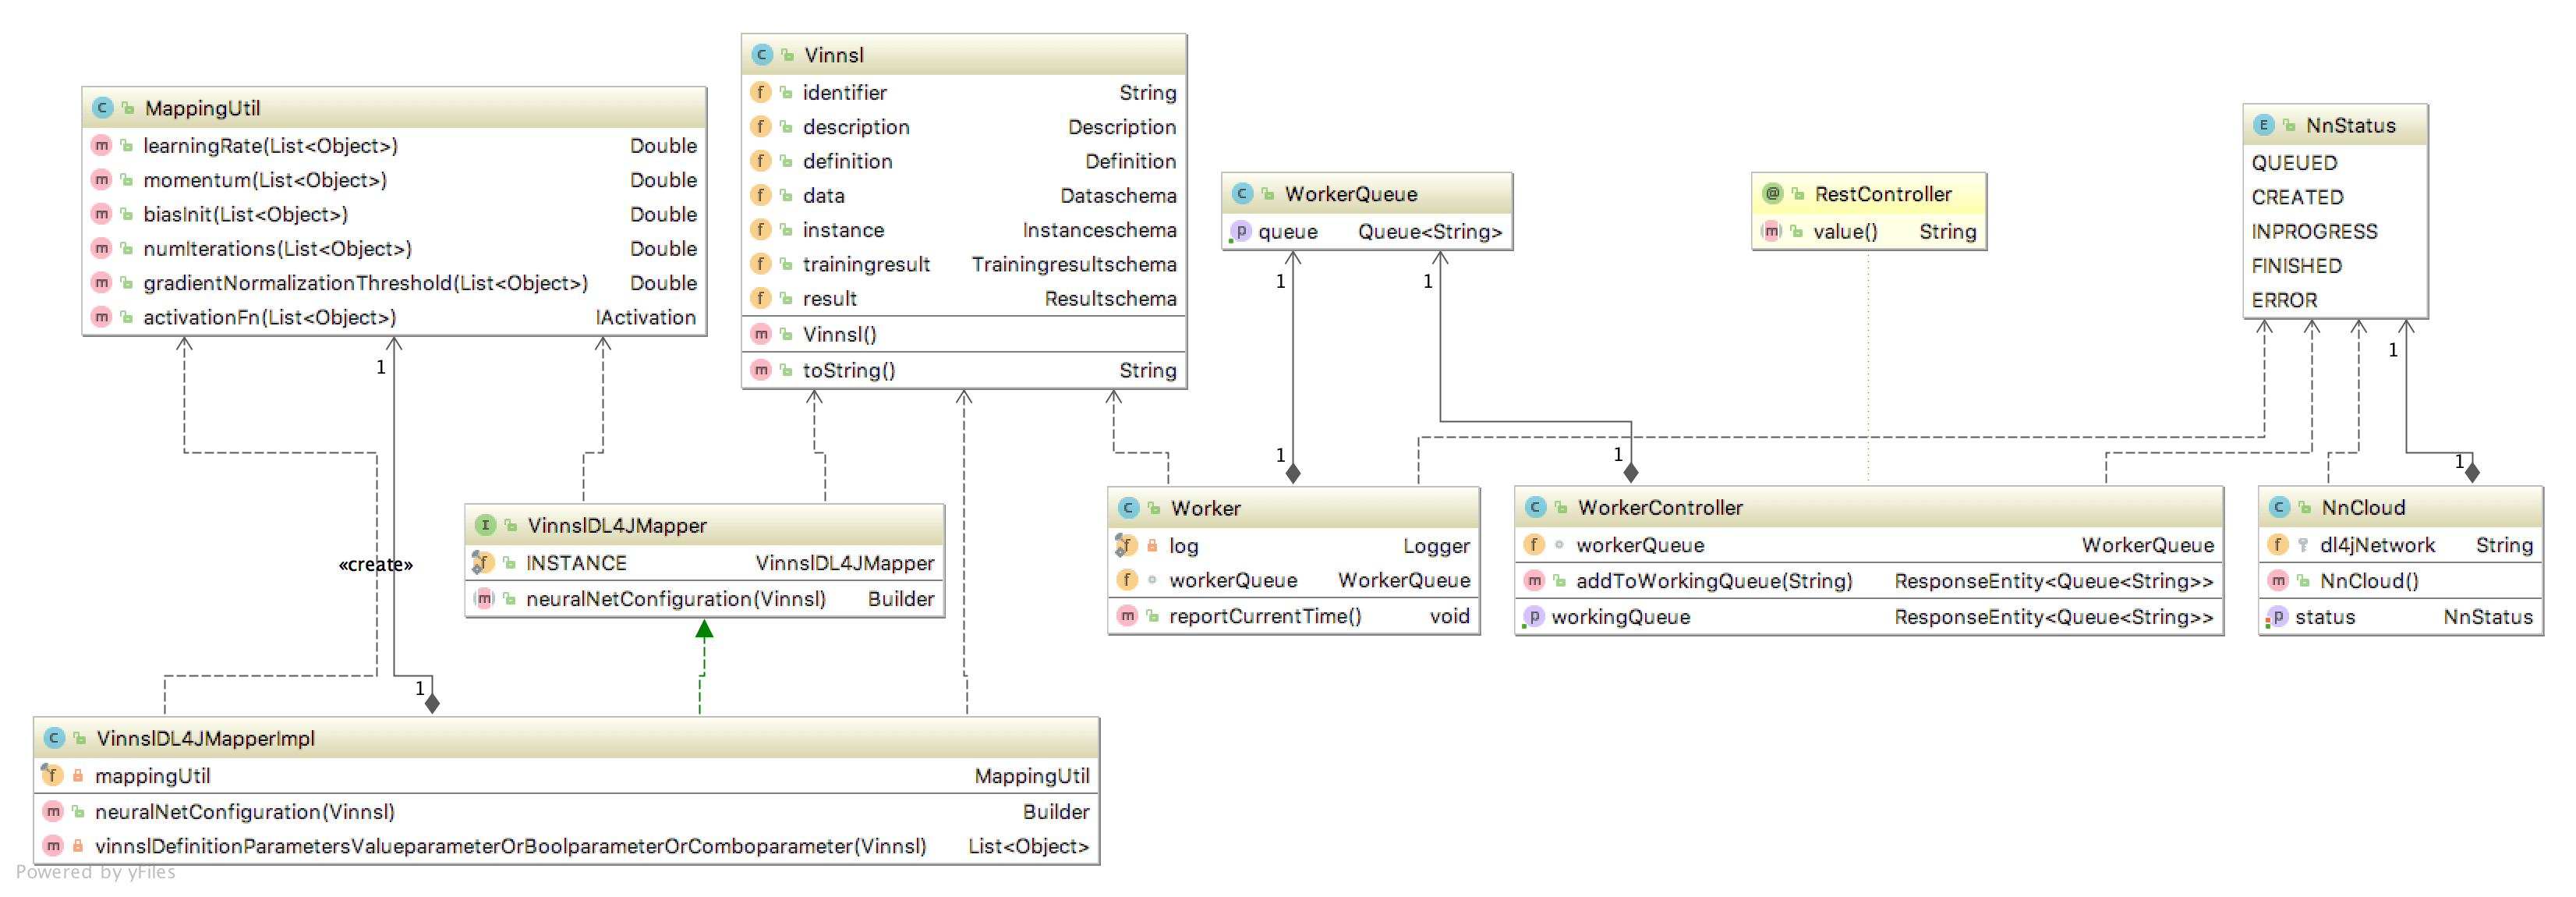
\includegraphics[width=17.00000cm]{images/uml-class-diagram-vinnsl-worker-service}
\caption{Class Diagram of vinnsl-worker-service
\label{class_vinnsl-worker-service}}
\end{figure}

\subsection{vinnsl-nn-ui}\label{vinnsl-nn-ui}

The frontend service consists of one single controller named
\texttt{VinnslUI}. The \texttt{getStatus()} method retrieves all and
neural network ids and their status. This is stored in
\texttt{vinnslList}. When selecting a neural network from the list, the
neural network object is loaded by executing \texttt{getDetailsById()}.
The response is stored in \texttt{currentVinnslItem}.

Figure \ref{vinnsl-nn-ui_class} gives an overview of the used methods
and stored variables.

\begin{figure}
\centering
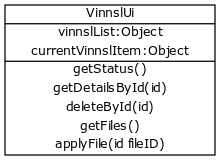
\includegraphics[width=6.00000cm]{images/vinnsl-nn-ui_class}
\caption{VinnslUI Vue Class \label{vinnsl-nn-ui_class}}
\end{figure}

\chapter{Prototype API Documentation}\label{prototype-api-documentation}

\paragraph{Base URL}\label{base-url}

\begin{verbatim}
http[s]://<clusterip>
\end{verbatim}

\section{vinnsl-service}\label{vinnsl-service-2}

\subsection{Import a new ViNNSL XML
Defintion}\label{import-a-new-vinnsl-xml-defintion}

\begin{verbatim}
POST /vinnsl
\end{verbatim}

\subsubsection{Parameters}\label{parameters}

\begin{longtable}[]{@{}llll@{}}
\toprule
Type & Name & Description & Schema\tabularnewline
\midrule
\endhead
\textbf{Body} & \textbf{vinnsl} \emph{required} & vinnsl &
Vinnsl\tabularnewline
\bottomrule
\end{longtable}

\subsubsection{Responses}\label{responses}

\begin{longtable}[]{@{}lll@{}}
\toprule
HTTP Code & Description & Schema\tabularnewline
\midrule
\endhead
\textbf{201} & Created & No Content\tabularnewline
\textbf{500} & Server Error & Error\tabularnewline
\bottomrule
\end{longtable}

\subsubsection{Consumes}\label{consumes}

\begin{itemize}
\tightlist
\item
  \texttt{application/xml}
\end{itemize}

\subsubsection{Produces}\label{produces}

\begin{itemize}
\tightlist
\item
  \texttt{*/*}
\end{itemize}

\subsubsection{Tags}\label{tags}

\begin{itemize}
\tightlist
\item
  vinnsl-service-controller
\end{itemize}

\subsubsection{Example HTTP request}\label{example-http-request}

\paragraph{Header}\label{header}

\begin{verbatim}
Content-Type: application/xml
\end{verbatim}

\paragraph{Body}\label{body}

\begin{verbatim}
<vinnsl>
  <description>
    <identifier><!-- will be generated --></identifier>
    <metadata>
      <paradigm>classification</paradigm>
      <name>Backpropagation Classification</name>
      <description>Iris Classification Example</description>
      <version>
        <major>1</major>
        <minor>0</minor>
      </version>
    </metadata>
    <creator>
      <name>Benjamin Nussbaum</name>
      <contact>nussbaum@institution.com</contact>
    </creator>
    <problemDomain>
      <propagationType type="feedforward">
        <learningType>supervised</learningType>
      </propagationType>
      <applicationField>Classification</applicationField>
      <networkType>Backpropagation</networkType>
      <problemType>Classifiers</problemType>
    </problemDomain>
    <endpoints>
      <train>true</train>
      <retrain>true</retrain>
      <evaluate>true</evaluate>
    </endpoints>
    <structure>
       <input>
        <ID>Input1</ID>
        <size>
            <min>4</min>
            <max>4</max>
        </size>
       </input>
       <hidden>
        <ID>Hidden1</ID>
        <size>
            <min>3</min>
            <max>3</max>
        </size>
       </hidden>
       <hidden>
        <ID>Hidden2</ID>
        <size>
            <min>3</min>
            <max>3</max>
        </size>
       </hidden>
       <output>
        <ID>Output1</ID>
        <size>
            <min>3</min>
            <max>3</max>
        </size>
       </output>
     </structure>
     <parameters/>
     <data>
        <description>iris txt file with 3 classifications, 4 input vars</description>
        <tabledescription>no input as table possible</tabledescription>
        <filedescription>CSV file</filedescription>
     </data>
  </description>
</vinnsl>
\end{verbatim}

\subsubsection{Example HTTP response}\label{example-http-response}

Statuscode: \texttt{201} CREATED

\paragraph{Header}\label{header-1}

\begin{verbatim}
Location: https://<baseURL>/vinnsl/5ade36bbd601800001206798
\end{verbatim}

\subsection{List all Neural Networks}\label{list-all-neural-networks}

\begin{verbatim}
GET /vinnsl
\end{verbatim}

\subsubsection{Responses}\label{responses-1}

\begin{longtable}[]{@{}lll@{}}
\toprule
HTTP Code & Description & Schema\tabularnewline
\midrule
\endhead
\textbf{200} & OK & \textless{} Vinnsl \textgreater{}
array\tabularnewline
\textbf{404} & Not Found & No Content\tabularnewline
\textbf{500} & Server Error & Error\tabularnewline
\bottomrule
\end{longtable}

\subsubsection{Produces}\label{produces-1}

\begin{itemize}
\tightlist
\item
  \texttt{application/json}
\end{itemize}

\subsubsection{Tags}\label{tags-1}

\begin{itemize}
\tightlist
\item
  vinnsl-service-controller
\end{itemize}

\subsubsection{Example HTTP Response}\label{example-http-response-1}

\begin{verbatim}
[
    {
        "identifier": "5ab91658e8cc45946600ea11",
        "description": {},
        "definition": {},
        "data": {},
        "instance": {},
        "trainingresult": {},
        "result": {},
        "nncloud": {
            "status": "CREATED",
            "dl4jNetwork": "{}
        }
    },
    ...
]
\end{verbatim}

\subsection{Delete all Neural
Networks}\label{delete-all-neural-networks}

\begin{verbatim}
DELETE /vinnsl/deleteall
\end{verbatim}

\subsubsection{Responses}\label{responses-2}

\begin{longtable}[]{@{}lll@{}}
\toprule
HTTP Code & Description & Schema\tabularnewline
\midrule
\endhead
\textbf{200} & OK & object\tabularnewline
\textbf{204} & No Content & No Content\tabularnewline
\textbf{500} & Server Error & Error\tabularnewline
\bottomrule
\end{longtable}

\subsubsection{Produces}\label{produces-2}

\begin{itemize}
\tightlist
\item
  \texttt{application/json}
\end{itemize}

\subsubsection{Tags}\label{tags-2}

\begin{itemize}
\tightlist
\item
  vinnsl-service-controller
\end{itemize}

\subsection{Get Neural Network Object}\label{get-neural-network-object}

\begin{verbatim}
GET /vinnsl/{id}
\end{verbatim}

\subsubsection{Parameters}\label{parameters-1}

\begin{longtable}[]{@{}llll@{}}
\toprule
Type & Name & Description & Schema\tabularnewline
\midrule
\endhead
\textbf{Path} & \textbf{id} \emph{required} & id & string\tabularnewline
\bottomrule
\end{longtable}

\subsubsection{Responses}\label{responses-3}

\begin{longtable}[]{@{}lll@{}}
\toprule
HTTP Code & Description & Schema\tabularnewline
\midrule
\endhead
\textbf{200} & OK & Vinnsl\tabularnewline
\textbf{404} & Not Found & No Content\tabularnewline
\bottomrule
\end{longtable}

\subsubsection{Produces}\label{produces-3}

\begin{itemize}
\tightlist
\item
  \texttt{application/xml}
\item
  \texttt{application/json}
\end{itemize}

\subsubsection{Tags}\label{tags-3}

\begin{itemize}
\tightlist
\item
  vinnsl-service-controller
\end{itemize}

\subsubsection{Example HTTP response}\label{example-http-response-2}

\begin{verbatim}
<?xml version="1.0" encoding="UTF-8" standalone="yes"?>
<vinnsl>
    <identifier>5ab91658e8cc45946600ea11</identifier>
    <description>
        <identifier></identifier>
        <metadata>
            <paradigm>classification</paradigm>
            <name>Backpropagation Classification</name>
            <description>Face Recognition Example</description>
            <version>
                <major>1</major>
                <minor>5</minor>
            </version>
        </metadata>
        <creator>
            <name>Autor 1</name>
            <contact>author1@institution.com</contact>
        </creator>
        <problemDomain>
            <propagationType type="feedforward">
                <learningType>supervised</learningType>
            </propagationType>
            <applicationField>EMS</applicationField>
            <applicationField>Operations</applicationField>
            <applicationField>FaceRecoginition</applicationField>
            <networkType>Backpropagation</networkType>
            <problemType>Classifiers</problemType>
        </problemDomain>
        <endpoints>
            <train>true</train>
            <retrain>true</retrain>
            <evaluate>true</evaluate>
        </endpoints>
        <structure>
            <input>
                <ID>Input1</ID>
                <dimension>
                    <min>1</min>
                    <max>1</max>
                </dimension>
                <size>
                    <min>960</min>
                    <max>960</max>
                </size>
            </input>
            <hidden>
                <ID>Hidden1</ID>
                <dimension>
                    <min>1</min>
                    <max>1024</max>
                </dimension>
            </hidden>
            <output>
                <ID>Output1</ID>
                <dimension>
                    <min>1</min>
                    <max>1</max>
                </dimension>
                <size>
                    <min>1</min>
                    <max>1</max>
                </size>
            </output>
        </structure>
        <parameters/>
        <data>
            <description>Input are face images with 32x30 px</description>
            <tabledescription>no input as table possible</tabledescription>
            <filedescription>prepare the input as file by reading the image files</filedescription>
        </data>
    </description>
    <definition>
        <identifier></identifier>
        <problemDomain>
            <propagationType type="feedforward">
                <learningType>supervised</learningType>
            </propagationType>
            <applicationField>EMS</applicationField>
            <applicationField>Operations</applicationField>
            <applicationField>FaceRecoginition</applicationField>
            <networkType>Backpropagation</networkType>
            <problemType>Classifiers</problemType>
        </problemDomain>
        <endpoints></endpoints>
        <executionEnvironment>
            <serial>true</serial>
        </executionEnvironment>
        <structure>
            <input>
                <ID>Input1</ID>
                <dimension>1</dimension>
                <size>960</size>
            </input>
            <hidden>
                <ID>Hidden1</ID>
                <dimension>1</dimension>
                <size>1024</size>
            </hidden>
            <output>
                <ID>Output1</ID>
                <dimension>1</dimension>
                <size>1</size>
            </output>
            <connections/>
        </structure>
        <resultSchema>
            <instance>true</instance>
            <training>true</training>
        </resultSchema>
        <parameters>
            <valueparameter name="learningrate">0.4</valueparameter>
            <valueparameter name="biasInput">1</valueparameter>
            <valueparameter name="biasHidden">1</valueparameter>
            <valueparameter name="momentum">0.1</valueparameter>
            <comboparameter name="ativationfunction">sigmoid</comboparameter>
            <valueparameter name="threshold">0.00001</valueparameter>
            <comboparameter name="activationfunction">sigmoid</comboparameter>
        </parameters>
        <data>
            <description>Input are face images with 32x30 px</description>
            <dataSchemaID>iris.txt</dataSchemaID>
        </data>
    </definition>
    <data>
        <identifier>5ab4e69c8f136a16bf81f093</identifier>
        <data>
            <file>5ab4e69c8f136a16bf81f093</file>
        </data>
    </data>
</vinnsl>
\end{verbatim}

\subsection{Remove Neural Network
Object}\label{remove-neural-network-object}

\begin{verbatim}
DELETE /vinnsl/{id}
\end{verbatim}

\subsubsection{Parameters}\label{parameters-2}

\begin{longtable}[]{@{}llll@{}}
\toprule
Type & Name & Description & Schema\tabularnewline
\midrule
\endhead
\textbf{Path} & \textbf{id} \emph{required} & id & string\tabularnewline
\bottomrule
\end{longtable}

\subsubsection{Responses}\label{responses-4}

\begin{longtable}[]{@{}lll@{}}
\toprule
HTTP Code & Description & Schema\tabularnewline
\midrule
\endhead
\textbf{200} & OK & ResponseEntity\tabularnewline
\textbf{204} & No Content & No Content\tabularnewline
\textbf{500} & Server Error & No Content\tabularnewline
\bottomrule
\end{longtable}

\subsubsection{Produces}\label{produces-4}

\begin{itemize}
\tightlist
\item
  \texttt{*/*}
\end{itemize}

\subsubsection{Tags}\label{tags-4}

\begin{itemize}
\tightlist
\item
  vinnsl-service-controller
\end{itemize}

\subsection{Add/Replace File of Neural
Network}\label{addreplace-file-of-neural-network}

\begin{verbatim}
PUT /vinnsl/{id}/addfile
\end{verbatim}

\subsubsection{Parameters}\label{parameters-3}

\begin{longtable}[]{@{}llll@{}}
\toprule
Type & Name & Description & Schema\tabularnewline
\midrule
\endhead
\textbf{Path} & \textbf{id} \emph{required} & id & string\tabularnewline
\textbf{Query} & \textbf{fileId} \emph{required} & fileId &
string\tabularnewline
\bottomrule
\end{longtable}

\subsubsection{Responses}\label{responses-5}

\begin{longtable}[]{@{}lll@{}}
\toprule
HTTP Code & Description & Schema\tabularnewline
\midrule
\endhead
\textbf{200} & OK & Vinnsl\tabularnewline
\textbf{404} & Not Found & No Content\tabularnewline
\textbf{500} & Server Error & Error\tabularnewline
\bottomrule
\end{longtable}

\subsubsection{Consumes}\label{consumes-1}

\begin{itemize}
\tightlist
\item
  \texttt{application/json}
\end{itemize}

\subsubsection{Produces}\label{produces-5}

\begin{itemize}
\tightlist
\item
  \texttt{application/xml}
\item
  \texttt{application/json}
\end{itemize}

\subsubsection{Tags}\label{tags-5}

\begin{itemize}
\tightlist
\item
  vinnsl-service-controller
\end{itemize}

\subsection{Add/Replace ViNNSL Definition of Neural
Network}\label{addreplace-vinnsl-definition-of-neural-network}

\begin{verbatim}
PUT /vinnsl/{id}/definition
\end{verbatim}

\subsubsection{Parameters}\label{parameters-4}

\begin{longtable}[]{@{}llll@{}}
\toprule
Type & Name & Description & Schema\tabularnewline
\midrule
\endhead
\textbf{Path} & \textbf{id} \emph{required} & id & string\tabularnewline
\textbf{Body} & \textbf{def} \emph{required} & def &
Definition\tabularnewline
\bottomrule
\end{longtable}

\subsubsection{Responses}\label{responses-6}

\begin{longtable}[]{@{}lll@{}}
\toprule
HTTP Code & Description & Schema\tabularnewline
\midrule
\endhead
\textbf{200} & OK & Vinnsl\tabularnewline
\textbf{404} & Not Found & No Content\tabularnewline
\textbf{500} & Server Error & Error\tabularnewline
\bottomrule
\end{longtable}

\subsubsection{Consumes}\label{consumes-2}

\begin{itemize}
\tightlist
\item
  \texttt{application/xml}
\item
  \texttt{application/json}
\end{itemize}

\subsubsection{Produces}\label{produces-6}

\begin{itemize}
\tightlist
\item
  \texttt{*/*}
\end{itemize}

\subsubsection{Tags}\label{tags-6}

\begin{itemize}
\tightlist
\item
  vinnsl-service-controller
\end{itemize}

\subsubsection{Example HTTP request}\label{example-http-request-1}

\paragraph{Request body}\label{request-body}

\begin{verbatim}
<definition>
<identifier><!-- will be generated --></identifier>
<metadata>
  <paradigm>classification</paradigm>
  <name>Backpropagation Classification</name>
  <description>Iris Classification Example</description>
  <version>
    <major>1</major>
    <minor>0</minor>
  </version>
</metadata>
<creator>
  <name>Ronald Fisher</name>
  <contact>ronald.fisher@institution.com</contact>
</creator>
<problemDomain>
  <propagationType type="feedforward">
    <learningType>supervised</learningType>
  </propagationType>
  <applicationField>Classification</applicationField>
  <networkType>Backpropagation</networkType>
  <problemType>Classifiers</problemType>
</problemDomain>
<endpoints>
  <train>true</train>
</endpoints>
<executionEnvironment>
    <serial>true</serial>
</executionEnvironment>
<structure>
   <input>
    <ID>Input1</ID>
    <size>4</size>
   </input>
   <hidden>
    <ID>Hidden1</ID>
    <size>3</size>
   </hidden>
   <hidden>
    <ID>Hidden2</ID>
    <size>3</size>
   </hidden>
   <output>
    <ID>Output1</ID>
    <size>3</size>
   </output>
   <connections>
    <!--<fullconnected>
        <fromblock>Input1</fromblock>
        <toblock>Hidden1</toblock>
        <fromblock>Hidden1</fromblock>
        <toblock>Output1</toblock>
    </fullconnected>-->
   </connections>
 </structure>
 <resultSchema>
    <instance>true</instance>
    <training>true</training>
 </resultSchema>
 <parameters>
    <valueparameter name="learningrate">0.1</valueparameter>
    <comboparameter name="activationfunction">tanh</comboparameter>
    <valueparameter name="iterations">500</valueparameter>
    <valueparameter name="seed">6</valueparameter>
 </parameters>
 <data>
    <description>iris txt file with 3 classifications, 4 input vars</description>
    <dataSchemaID>name/iris.txt</dataSchemaID>
 </data>
</definition>
\end{verbatim}

\subsection{Add/Replace ViNNSL Instanceschema of Neural
Network}\label{addreplace-vinnsl-instanceschema-of-neural-network}

\begin{verbatim}
PUT /vinnsl/{id}/instanceschema
\end{verbatim}

\subsubsection{Parameters}\label{parameters-5}

\begin{longtable}[]{@{}llll@{}}
\toprule
Type & Name & Description & Schema\tabularnewline
\midrule
\endhead
\textbf{Path} & \textbf{id} \emph{required} & id & string\tabularnewline
\textbf{Body} & \textbf{instance} \emph{required} & instance &
Instanceschema\tabularnewline
\bottomrule
\end{longtable}

\subsubsection{Responses}\label{responses-7}

\begin{longtable}[]{@{}lll@{}}
\toprule
HTTP Code & Description & Schema\tabularnewline
\midrule
\endhead
\textbf{200} & OK & object\tabularnewline
\textbf{404} & Not Found & No Content\tabularnewline
\textbf{500} & Server Error & Error\tabularnewline
\bottomrule
\end{longtable}

\subsubsection{Consumes}\label{consumes-3}

\begin{itemize}
\tightlist
\item
  \texttt{application/xml}
\item
  \texttt{application/json}
\end{itemize}

\subsubsection{Produces}\label{produces-7}

\begin{itemize}
\tightlist
\item
  \texttt{*/*}
\end{itemize}

\subsubsection{Tags}\label{tags-7}

\begin{itemize}
\tightlist
\item
  vinnsl-service-controller
\end{itemize}

\subsubsection{Example HTTP request}\label{example-http-request-2}

\paragraph{Request body}\label{request-body-1}

\begin{verbatim}
<instanceschema>
</instanceschema>
\end{verbatim}

\subsection{Add/Replace ViNNSL Resultschema of Neural
Network}\label{addreplace-vinnsl-resultschema-of-neural-network}

\begin{verbatim}
PUT /vinnsl/{id}/resultschema
\end{verbatim}

\subsubsection{Parameters}\label{parameters-6}

\begin{longtable}[]{@{}llll@{}}
\toprule
Type & Name & Description & Schema\tabularnewline
\midrule
\endhead
\textbf{Path} & \textbf{id} \emph{required} & id & string\tabularnewline
\textbf{Body} & \textbf{resultSchema} \emph{required} & resultSchema &
Resultschema\tabularnewline
\bottomrule
\end{longtable}

\subsubsection{Responses}\label{responses-8}

\begin{longtable}[]{@{}lll@{}}
\toprule
HTTP Code & Description & Schema\tabularnewline
\midrule
\endhead
\textbf{200} & OK & object\tabularnewline
\textbf{404} & Not Found & No Content\tabularnewline
\textbf{500} & Server Error & Error\tabularnewline
\bottomrule
\end{longtable}

\subsubsection{Consumes}\label{consumes-4}

\begin{itemize}
\tightlist
\item
  \texttt{application/xml}
\item
  \texttt{application/json}
\end{itemize}

\subsubsection{Produces}\label{produces-8}

\begin{itemize}
\tightlist
\item
  \texttt{*/*}
\end{itemize}

\subsubsection{Tags}\label{tags-8}

\begin{itemize}
\tightlist
\item
  vinnsl-service-controller
\end{itemize}

\subsubsection{Example HTTP request}\label{example-http-request-3}

\paragraph{Request body}\label{request-body-2}

\begin{verbatim}
<resultschema>
</resultschema>
\end{verbatim}

\subsection{Add/Replace ViNNSL Trainingresult of Neural
Network}\label{addreplace-vinnsl-trainingresult-of-neural-network}

\begin{verbatim}
PUT /vinnsl/{id}/trainingresult
\end{verbatim}

\subsubsection{Parameters}\label{parameters-7}

\begin{longtable}[]{@{}llll@{}}
\toprule
Type & Name & Description & Schema\tabularnewline
\midrule
\endhead
\textbf{Path} & \textbf{id} \emph{required} & id & string\tabularnewline
\textbf{Body} & \textbf{trainingresult} \emph{required} & trainingresult
& Trainingresultschema\tabularnewline
\bottomrule
\end{longtable}

\subsubsection{Responses}\label{responses-9}

\begin{longtable}[]{@{}lll@{}}
\toprule
HTTP Code & Description & Schema\tabularnewline
\midrule
\endhead
\textbf{200} & OK & object\tabularnewline
\textbf{404} & Not Found & No Content\tabularnewline
\textbf{500} & Server Error & Error\tabularnewline
\bottomrule
\end{longtable}

\subsubsection{Consumes}\label{consumes-5}

\begin{itemize}
\tightlist
\item
  \texttt{application/xml}
\item
  \texttt{application/json}
\end{itemize}

\subsubsection{Produces}\label{produces-9}

\begin{itemize}
\tightlist
\item
  \texttt{*/*}
\end{itemize}

\subsubsection{Tags}\label{tags-9}

\begin{itemize}
\tightlist
\item
  vinnsl-service-controller
\end{itemize}

\subsubsection{Example HTTP request}\label{example-http-request-4}

\paragraph{Request body}\label{request-body-3}

\begin{verbatim}
<trainingresult>
</trainingresult>
\end{verbatim}

\subsection{Get Status of all Neural
Networks}\label{get-status-of-all-neural-networks}

\begin{verbatim}
GET /status
\end{verbatim}

\subsubsection{Responses}\label{responses-10}

\begin{longtable}[]{@{}lll@{}}
\toprule
HTTP Code & Description & Schema\tabularnewline
\midrule
\endhead
\textbf{200} & OK & object\tabularnewline
\textbf{404} & Not Found & No Content\tabularnewline
\bottomrule
\end{longtable}

\subsubsection{Produces}\label{produces-10}

\begin{itemize}
\tightlist
\item
  \texttt{application/json}
\end{itemize}

\subsubsection{Tags}\label{tags-10}

\begin{itemize}
\tightlist
\item
  nn-status-controller
\end{itemize}

\subsubsection{HTTP response example}\label{http-response-example}

\begin{verbatim}
{
    "5ab91658e8cc45946600ea11": "INPROGRESS"
}
\end{verbatim}

\subsection{Get Status of Neural
Network}\label{get-status-of-neural-network}

\begin{verbatim}
GET /status/{id}
\end{verbatim}

\subsubsection{Parameters}\label{parameters-8}

\begin{longtable}[]{@{}llll@{}}
\toprule
Type & Name & Description & Schema\tabularnewline
\midrule
\endhead
\textbf{Path} & \textbf{id} \emph{required} & id & string\tabularnewline
\bottomrule
\end{longtable}

\subsubsection{Responses}\label{responses-11}

\begin{longtable}[]{@{}lll@{}}
\toprule
HTTP Code & Description & Schema\tabularnewline
\midrule
\endhead
\textbf{200} & OK & object\tabularnewline
\textbf{404} & Not Found & No Content\tabularnewline
\bottomrule
\end{longtable}

\subsubsection{Produces}\label{produces-11}

\begin{itemize}
\tightlist
\item
  \texttt{application/json}
\end{itemize}

\subsubsection{Tags}\label{tags-11}

\begin{itemize}
\tightlist
\item
  nn-status-controller
\end{itemize}

\subsection{Set Status of a Neural
Network}\label{set-status-of-a-neural-network}

\begin{verbatim}
PUT /status/{id}/{status}
\end{verbatim}

\subsubsection{Parameters}\label{parameters-9}

\begin{longtable}[]{@{}llll@{}}
\toprule
\begin{minipage}[b]{0.08\columnwidth}\raggedright\strut
Type\strut
\end{minipage} & \begin{minipage}[b]{0.21\columnwidth}\raggedright\strut
Name\strut
\end{minipage} & \begin{minipage}[b]{0.11\columnwidth}\raggedright\strut
Description\strut
\end{minipage} & \begin{minipage}[b]{0.49\columnwidth}\raggedright\strut
Schema\strut
\end{minipage}\tabularnewline
\midrule
\endhead
\begin{minipage}[t]{0.08\columnwidth}\raggedright\strut
\textbf{Path}\strut
\end{minipage} & \begin{minipage}[t]{0.21\columnwidth}\raggedright\strut
\textbf{id} \emph{required}\strut
\end{minipage} & \begin{minipage}[t]{0.11\columnwidth}\raggedright\strut
id\strut
\end{minipage} & \begin{minipage}[t]{0.49\columnwidth}\raggedright\strut
string\strut
\end{minipage}\tabularnewline
\begin{minipage}[t]{0.08\columnwidth}\raggedright\strut
\textbf{Path}\strut
\end{minipage} & \begin{minipage}[t]{0.21\columnwidth}\raggedright\strut
\textbf{status} \emph{required}\strut
\end{minipage} & \begin{minipage}[t]{0.11\columnwidth}\raggedright\strut
status\strut
\end{minipage} & \begin{minipage}[t]{0.49\columnwidth}\raggedright\strut
enum (\texttt{CREATED,\ QUEUED,\ INPROGRESS,\ FINISHED,\ ERROR})\strut
\end{minipage}\tabularnewline
\bottomrule
\end{longtable}

\subsubsection{Responses}\label{responses-12}

\begin{longtable}[]{@{}lll@{}}
\toprule
HTTP Code & Description & Schema\tabularnewline
\midrule
\endhead
\textbf{200} & OK & object\tabularnewline
\textbf{404} & Not Found & No Content\tabularnewline
\textbf{500} & Server Error & Error\tabularnewline
\bottomrule
\end{longtable}

\subsubsection{Consumes}\label{consumes-6}

\begin{itemize}
\tightlist
\item
  \texttt{application/json}
\end{itemize}

\subsubsection{Produces}\label{produces-12}

\begin{itemize}
\tightlist
\item
  \texttt{application/json}
\end{itemize}

\subsubsection{Tags}\label{tags-12}

\begin{itemize}
\tightlist
\item
  nn-status-controller
\end{itemize}

\subsection{Get Deeplearning4J Transformation Object of Neural
Network}\label{get-deeplearning4j-transformation-object-of-neural-network}

\begin{verbatim}
GET /dl4j/{id}
\end{verbatim}

\subsubsection{Parameters}\label{parameters-10}

\begin{longtable}[]{@{}llll@{}}
\toprule
Type & Name & Description & Schema\tabularnewline
\midrule
\endhead
\textbf{Path} & \textbf{id} \emph{required} & id & string\tabularnewline
\bottomrule
\end{longtable}

\subsubsection{Responses}\label{responses-13}

\begin{longtable}[]{@{}lll@{}}
\toprule
HTTP Code & Description & Schema\tabularnewline
\midrule
\endhead
\textbf{200} & OK & string\tabularnewline
\textbf{404} & Not Found & No Content\tabularnewline
\bottomrule
\end{longtable}

\subsubsection{Produces}\label{produces-13}

\begin{itemize}
\tightlist
\item
  \texttt{application/json}
\end{itemize}

\subsubsection{Tags}\label{tags-13}

\begin{itemize}
\tightlist
\item
  dl4j-service-controller
\end{itemize}

\subsection{Put Deeplearning4J Transformation Object of Neural
Network}\label{put-deeplearning4j-transformation-object-of-neural-network}

\begin{verbatim}
PUT /dl4j/{id}
\end{verbatim}

\subsubsection{Parameters}\label{parameters-11}

\begin{longtable}[]{@{}llll@{}}
\toprule
Type & Name & Description & Schema\tabularnewline
\midrule
\endhead
\textbf{Path} & \textbf{id} \emph{required} & id & string\tabularnewline
\textbf{Body} & \textbf{dl4J} \emph{required} & dl4J &
string\tabularnewline
\bottomrule
\end{longtable}

\subsubsection{Responses}\label{responses-14}

\begin{longtable}[]{@{}lll@{}}
\toprule
HTTP Code & Description & Schema\tabularnewline
\midrule
\endhead
\textbf{200} & OK & ResponseEntity\tabularnewline
\textbf{404} & Not Found & No Content\tabularnewline
\textbf{500} & Server Error & Error\tabularnewline
\bottomrule
\end{longtable}

\subsubsection{Consumes}\label{consumes-7}

\begin{itemize}
\tightlist
\item
  \texttt{application/json}
\end{itemize}

\subsubsection{Produces}\label{produces-14}

\begin{itemize}
\tightlist
\item
  \texttt{application/json}
\end{itemize}

\subsubsection{Tags}\label{tags-14}

\begin{itemize}
\tightlist
\item
  dl-4j-service-controller
\end{itemize}

\section{vinnsl-storage-service}\label{vinnsl-storage-service-1}

\subsection{Handle File Upload from HTML
Form}\label{handle-file-upload-from-html-form}

\begin{verbatim}
POST /storage
\end{verbatim}

\subsubsection{Parameters}\label{parameters-12}

\begin{longtable}[]{@{}llll@{}}
\toprule
Type & Name & Description & Schema\tabularnewline
\midrule
\endhead
\textbf{FormData} & \textbf{file} \emph{required} & file &
file\tabularnewline
\bottomrule
\end{longtable}

\subsubsection{Responses}\label{responses-15}

\begin{longtable}[]{@{}lll@{}}
\toprule
HTTP Code & Description & Schema\tabularnewline
\midrule
\endhead
\textbf{200} & OK & string\tabularnewline
\textbf{201} & Created & No Content\tabularnewline
\textbf{404} & Not Found & No Content\tabularnewline
\bottomrule
\end{longtable}

\subsubsection{Consumes}\label{consumes-8}

\begin{itemize}
\tightlist
\item
  \texttt{multipart/form-data}
\end{itemize}

\subsubsection{Produces}\label{produces-15}

\begin{itemize}
\tightlist
\item
  \texttt{\textbackslash{}*/*}
\end{itemize}

\subsubsection{Tags}\label{tags-15}

\begin{itemize}
\tightlist
\item
  vinnsl-storage-controller
\end{itemize}

\subsection{List all Files}\label{list-all-files}

\begin{verbatim}
GET /storage
\end{verbatim}

\subsubsection{Responses}\label{responses-16}

\begin{longtable}[]{@{}lll@{}}
\toprule
HTTP Code & Description & Schema\tabularnewline
\midrule
\endhead
\textbf{200} & OK & \protect\hyperlink{model}{Model}\tabularnewline
\textbf{404} & Not Found & No Content\tabularnewline
\bottomrule
\end{longtable}

\subsubsection{Produces}\label{produces-16}

\begin{itemize}
\tightlist
\item
  \texttt{application/json}
\end{itemize}

\subsubsection{Tags}\label{tags-16}

\begin{itemize}
\tightlist
\item
  vinnsl-storage-controller
\end{itemize}

\subsection{Download File by Original
Filename}\label{download-file-by-original-filename}

\begin{verbatim}
GET /storage/files/name/{filename}
\end{verbatim}

\subsubsection{Parameters}\label{parameters-13}

\begin{longtable}[]{@{}llll@{}}
\toprule
Type & Name & Description & Schema\tabularnewline
\midrule
\endhead
\textbf{Path} & \textbf{filename} \emph{required} & filename &
string\tabularnewline
\bottomrule
\end{longtable}

\subsubsection{Responses}\label{responses-17}

\begin{longtable}[]{@{}lll@{}}
\toprule
HTTP Code & Description & Schema\tabularnewline
\midrule
\endhead
\textbf{200} & OK & string (byte)\tabularnewline
\textbf{404} & Not Found & No Content\tabularnewline
\bottomrule
\end{longtable}

\subsubsection{Produces}\label{produces-17}

\begin{itemize}
\tightlist
\item
  \texttt{\textbackslash{}*/*}
\end{itemize}

\subsubsection{Tags}\label{tags-17}

\begin{itemize}
\tightlist
\item
  vinnsl-storage-controller
\end{itemize}

\subsection{Download or Show File by
FileID}\label{download-or-show-file-by-fileid}

\begin{verbatim}
GET /storage/files/{fileId}
\end{verbatim}

\subsubsection{Parameters}\label{parameters-14}

\begin{longtable}[]{@{}llll@{}}
\toprule
Type & Name & Description & Schema\tabularnewline
\midrule
\endhead
\textbf{Path} & \textbf{fileId} \emph{required} & fileId &
string\tabularnewline
\textbf{Query} & \textbf{download} \emph{optional} & download &
boolean\tabularnewline
\bottomrule
\end{longtable}

\subsubsection{Responses}\label{responses-18}

\begin{longtable}[]{@{}lll@{}}
\toprule
HTTP Code & Description & Schema\tabularnewline
\midrule
\endhead
\textbf{200} & OK & string (byte)\tabularnewline
\textbf{404} & Not Found & No Content\tabularnewline
\bottomrule
\end{longtable}

\subsubsection{Produces}\label{produces-18}

\begin{itemize}
\tightlist
\item
  \texttt{\textbackslash{}*/*}
\end{itemize}

\subsubsection{Tags}\label{tags-18}

\begin{itemize}
\tightlist
\item
  vinnsl-storage-controller
\end{itemize}

\subsection{Delete File by FileID}\label{delete-file-by-fileid}

\begin{verbatim}
DELETE /storage/files/{fileId}
\end{verbatim}

\subsubsection{Parameters}\label{parameters-15}

\begin{longtable}[]{@{}llll@{}}
\toprule
Type & Name & Description & Schema\tabularnewline
\midrule
\endhead
\textbf{Path} & \textbf{fileId} \emph{required} & fileId &
string\tabularnewline
\bottomrule
\end{longtable}

\subsubsection{Responses}\label{responses-19}

\begin{longtable}[]{@{}lll@{}}
\toprule
HTTP Code & Description & Schema\tabularnewline
\midrule
\endhead
\textbf{200} & OK & ResponseEntity\tabularnewline
\textbf{204} & No Content & No Content\tabularnewline
\textbf{403} & Forbidden & No Content\tabularnewline
\bottomrule
\end{longtable}

\subsubsection{Produces}\label{produces-19}

\begin{itemize}
\tightlist
\item
  \texttt{\textbackslash{}*/*}
\end{itemize}

\subsubsection{Tags}\label{tags-19}

\begin{itemize}
\tightlist
\item
  vinnsl-storage-controller
\end{itemize}

\subsection{Get File Metadata by
FileID}\label{get-file-metadata-by-fileid}

\begin{verbatim}
GET /storage/metadata/{fileId}
\end{verbatim}

\subsubsection{Parameters}\label{parameters-16}

\begin{longtable}[]{@{}llll@{}}
\toprule
Type & Name & Description & Schema\tabularnewline
\midrule
\endhead
\textbf{Path} & \textbf{fileId} \emph{required} & fileId &
string\tabularnewline
\bottomrule
\end{longtable}

\subsubsection{Responses}\label{responses-20}

\begin{longtable}[]{@{}lll@{}}
\toprule
HTTP Code & Description & Schema\tabularnewline
\midrule
\endhead
\textbf{200} & OK & \textless{} string, object \textgreater{}
map\tabularnewline
\textbf{404} & Not Found & No Content\tabularnewline
\bottomrule
\end{longtable}

\subsubsection{Produces}\label{produces-20}

\begin{itemize}
\tightlist
\item
  \texttt{\textbackslash{}*/*}
\end{itemize}

\subsubsection{Tags}\label{tags-20}

\begin{itemize}
\tightlist
\item
  vinnsl-storage-controller
\end{itemize}

\subsection{Upload MultipartFile}\label{upload-multipartfile}

\begin{verbatim}
POST /storage/upload
\end{verbatim}

\subsubsection{Parameters}\label{parameters-17}

\begin{longtable}[]{@{}llll@{}}
\toprule
Type & Name & Description & Schema\tabularnewline
\midrule
\endhead
\textbf{FormData} & \textbf{file} \emph{required} & file &
file\tabularnewline
\bottomrule
\end{longtable}

\subsubsection{Responses}\label{responses-21}

\begin{longtable}[]{@{}lll@{}}
\toprule
HTTP Code & Description & Schema\tabularnewline
\midrule
\endhead
\textbf{200} & OK & object\tabularnewline
\textbf{201} & Created & No Content\tabularnewline
\textbf{404} & Not Found & No Content\tabularnewline
\bottomrule
\end{longtable}

\subsubsection{Consumes}\label{consumes-9}

\begin{itemize}
\tightlist
\item
  \texttt{multipart/form-data}
\end{itemize}

\subsubsection{Produces}\label{produces-21}

\begin{itemize}
\tightlist
\item
  \texttt{application/json}
\end{itemize}

\subsubsection{Tags}\label{tags-21}

\begin{itemize}
\tightlist
\item
  vinnsl-storage-controller
\end{itemize}

\subsection{Upload File by URL}\label{upload-file-by-url}

\begin{verbatim}
GET /storage/upload
\end{verbatim}

\subsubsection{Parameters}\label{parameters-18}

\begin{longtable}[]{@{}llll@{}}
\toprule
Type & Name & Description & Schema\tabularnewline
\midrule
\endhead
\textbf{Query} & \textbf{url} \emph{required} & url &
string\tabularnewline
\bottomrule
\end{longtable}

\subsubsection{Responses}\label{responses-22}

\begin{longtable}[]{@{}lll@{}}
\toprule
HTTP Code & Description & Schema\tabularnewline
\midrule
\endhead
\textbf{200} & OK & object\tabularnewline
\textbf{404} & Not Found & No Content\tabularnewline
\bottomrule
\end{longtable}

\subsubsection{Produces}\label{produces-22}

\begin{itemize}
\tightlist
\item
  \texttt{application/json}
\end{itemize}

\subsubsection{Tags}\label{tags-22}

\begin{itemize}
\tightlist
\item
  vinnsl-storage-controller
\end{itemize}

\section{vinnsl-worker-service}\label{vinnsl-worker-service-1}

\subsection{getWorkingQueue}\label{getworkingqueue}

\begin{verbatim}
GET /worker/queue
\end{verbatim}

\subsubsection{Responses}\label{responses-23}

\begin{longtable}[]{@{}lll@{}}
\toprule
HTTP Code & Description & Schema\tabularnewline
\midrule
\endhead
\textbf{200} & OK & \textless{} string \textgreater{}
array\tabularnewline
\textbf{401} & Unauthorized & No Content\tabularnewline
\textbf{403} & Forbidden & No Content\tabularnewline
\textbf{404} & Not Found & No Content\tabularnewline
\bottomrule
\end{longtable}

\subsubsection{Produces}\label{produces-23}

\begin{itemize}
\tightlist
\item
  \texttt{\textbackslash{}*/*}
\end{itemize}

\subsubsection{Tags}\label{tags-23}

\begin{itemize}
\tightlist
\item
  worker-controller
\end{itemize}

\subsection{addToWorkingQueue}\label{addtoworkingqueue}

\begin{verbatim}
PUT /worker/queue/{id}
\end{verbatim}

\subsubsection{Parameters}\label{parameters-19}

\begin{longtable}[]{@{}llll@{}}
\toprule
Type & Name & Description & Schema\tabularnewline
\midrule
\endhead
\textbf{Path} & \textbf{id} \emph{required} & id & string\tabularnewline
\bottomrule
\end{longtable}

\subsubsection{Responses}\label{responses-24}

\begin{longtable}[]{@{}lll@{}}
\toprule
HTTP Code & Description & Schema\tabularnewline
\midrule
\endhead
\textbf{200} & OK & \textless{} string \textgreater{}
array\tabularnewline
\textbf{201} & Created & No Content\tabularnewline
\textbf{401} & Unauthorized & No Content\tabularnewline
\textbf{403} & Forbidden & No Content\tabularnewline
\textbf{404} & Not Found & No Content\tabularnewline
\bottomrule
\end{longtable}

\subsubsection{Consumes}\label{consumes-10}

\begin{itemize}
\tightlist
\item
  \texttt{application/json}
\end{itemize}

\subsubsection{Produces}\label{produces-24}

\begin{itemize}
\tightlist
\item
  \texttt{application/json}
\end{itemize}

\subsubsection{Tags}\label{tags-24}

\begin{itemize}
\tightlist
\item
  worker-controller
\end{itemize}

\chapter{Use Cases}\label{use-cases}

As demonstration of the implemented prototype this thesis features two
use cases with practical relevance.

\section{Iris Classification Example}\label{iris-classification-example}

Ronald A. Fisher published 1936 in his paper \emph{The use of multiple
measurements in taxonomic problems} \cite{fisher} a dataset that is
known as the \emph{Iris flower data set}.

The data set \cite{fisher} features 50 examples of three Iris species:
Iris setosa, Iris virginica and Iris versicolor. A table lists four
measured features from each sample: the length and the width of the
sepals and petals.

This use case shall showcase the use of the implemented prototype to
create a neural network, train and evaluate it, using this dataset.

\subsection{Dataset}\label{dataset}

The dataset exists in the UCI Machine Learning Repository
\cite{uci-iris} as a \emph{CSV} (comma separated value) file\footnote{https://archive.ics.uci.edu/ml/datasets/iris}
which will be used for training. The first example has a sepal
length/width of 5.1cm/3.5cm, a petal length/width of 1.4cm/0.2cm and is
an Iris setosa.

The first lines of the dataset explain the structure of the dataset. The
columns are formatted for better readability. The species column is an
enumerated value.

\begin{longtable}[]{@{}ll@{}}
\toprule
Index & Iris species\tabularnewline
\midrule
\endhead
0 & Iris setosa\tabularnewline
1 & Iris virginica\tabularnewline
2 & Iris versicolor\tabularnewline
\bottomrule
\end{longtable}

\begin{verbatim}
Sepal length, Sepal width, Petal length, Peta width, Iris species
5.1         , 3.5        , 1.4         , 0.2       , 0
4.9         , 3.0        , 1.4         , 0.2       , 0
<more lines>
\end{verbatim}

\subsection{Prerequisites}\label{prerequisites}

\begin{itemize}
\tightlist
\item
  Kubernetes Cluster running
\item
  Services from the Neural Network Execution Stack deployed in cluster
\item
  Hostname \texttt{cluster.local} resolves to Minikube instance
\end{itemize}

\subsection{Create the neural network}\label{create-the-neural-network}

\subsubsection{Request}\label{request}

\begin{verbatim}
POST https://cluster.local/vinnsl
\end{verbatim}

BODY

\begin{verbatim}
<vinnsl>
  <description>
    <identifier><!-- will be generated --></identifier>
    <metadata>
      <paradigm>classification</paradigm>
      <name>Backpropagation Classification</name>
      <description>Iris Classification Example</description>
      <version>
        <major>1</major>
        <minor>0</minor>
      </version>
    </metadata>
    <creator>
      <name>Ronald Fisher</name>
      <contact>ronald.fisher@institution.com</contact>
    </creator>
    <problemDomain>
      <propagationType type="feedforward">
        <learningType>supervised</learningType>
      </propagationType>
      <applicationField>Classification</applicationField>
      <networkType>Backpropagation</networkType>
      <problemType>Classifiers</problemType>
    </problemDomain>
    <endpoints>
      <train>true</train>
      <retrain>true</retrain>
      <evaluate>true</evaluate>
    </endpoints>
    <structure>
       <input>
        <ID>Input1</ID>
        <size>
            <min>4</min>
            <max>4</max>
        </size>
       </input>
       <hidden>
        <ID>Hidden1</ID>
        <size>
            <min>3</min>
            <max>3</max>
        </size>
       </hidden>
       <hidden>
        <ID>Hidden2</ID>
        <size>
            <min>3</min>
            <max>3</max>
        </size>
       </hidden>
       <output>
        <ID>Output1</ID>
        <size>
            <min>3</min>
            <max>3</max>
        </size>
       </output>
     </structure>
     <parameters>
        <valueparameter>learningrate</valueparameter>
        <valueparameter>biasInput</valueparameter>
        <valueparameter>biasHidden</valueparameter>
        <valueparameter>momentum</valueparameter>
        <comboparameter>ativationfunction</valueparameter>
        <valueparameter>threshold</valueparameter>
     </parameters>
     <data>
        <description>iris txt file with 3 classifications, 4 input vars</description>
        <tabledescription>no input as table possible</tabledescription>
        <filedescription>CSV file</filedescription>
     </data>
  </description>
</vinnsl>
\end{verbatim}

\subsubsection{Response}\label{response}

\begin{verbatim}
201 CREATED 
\end{verbatim}

Aside from the HTTP Status Code, we also get HTTP headers in the
response. The one needed for further requests is named
\texttt{location}. The value of this field is the URL of the network
that was created and can be used to get and update fields on the
dataset.

In this example the following value is returned:

\begin{longtable}[]{@{}ll@{}}
\toprule
Header Name & Header Value\tabularnewline
\midrule
\endhead
location &
https://cluster.local/vinnsl/5b1811a046e0fb0001fa28cc\tabularnewline
\bottomrule
\end{longtable}

The id of the new dataset is 5b1811a046e0fb0001fa28cc. In the following
requests the id is shortened as \texttt{\{id\}}.

\subsection{Add ViNNSL Definition to the neural
network}\label{add-vinnsl-definition-to-the-neural-network}

The ViNNSL definition XML contains metadata like name and description of
the network as well as the stucture of the neural network model. There
is one input and one output layer defined. In between there are two
hidden layers. It is also possible to specify additional parameters.

The activation function is set to Tangens hyperbolicus, the learning
rate is 0.1 and the training is limited to 500 iterations. A seed, set
to 6, allows reproducable training score.

\subsubsection{Request}\label{request-1}

\begin{verbatim}
POST https://cluster.local/vinnsl/{id}/definition
\end{verbatim}

BODY

\begin{verbatim}
<definition>
<identifier><!-- will be generated --></identifier>
<metadata>
  <paradigm>classification</paradigm>
  <name>Backpropagation Classification</name>
  <description>Iris Classification Example</description>
  <version>
    <major>1</major>
    <minor>0</minor>
  </version>
</metadata>
<creator>
  <name>Ronald Fisher</name>
  <contact>ronald.fisher@institution.com</contact>
</creator>
<problemDomain>
  <propagationType type="feedforward">
    <learningType>supervised</learningType>
  </propagationType>
  <applicationField>Classification</applicationField>
  <networkType>Backpropagation</networkType>
  <problemType>Classifiers</problemType>
</problemDomain>
<endpoints>
  <train>true</train>
</endpoints>
<executionEnvironment>
    <serial>true</serial>
</executionEnvironment>
<structure>
   <input>
    <ID>Input1</ID>
    <size>4</size>
   </input>
   <hidden>
    <ID>Hidden1</ID>
    <size>3</size>
   </hidden>
   <hidden>
    <ID>Hidden2</ID>
    <size>3</size>
   </hidden>
   <output>
    <ID>Output1</ID>
    <size>3</size>
   </output>
   <connections>
    <fullconnected>
        <fromblock>Input1</fromblock>
        <toblock>Hidden1</toblock>
        <fromblock>Hidden1</fromblock>
        <toblock>Output1</toblock>
    </fullconnected>
   </connections>
 </structure>
 <resultSchema>
    <instance>true</instance>
    <training>true</training>
 </resultSchema>
 <parameters>
    <valueparameter name="learningrate">0.1</valueparameter>
    <comboparameter name="activationfunction">tanh</comboparameter>
    <valueparameter name="iterations">500</valueparameter>
    <valueparameter name="seed">6</valueparameter>
 </parameters>
 <data>
    <description>iris txt file with 3 classifications, 4 input vars</description>
    <dataSchemaID>name/iris.txt</dataSchemaID>
 </data>
</definition>
\end{verbatim}

\subsubsection{Response}\label{response-1}

\begin{verbatim}
200 OK
\end{verbatim}

Figure \ref{usecase_1_datastructure} shows a graphical visualisation of
the neural network data structure after adding the description and
definition in \emph{ViNNSL} XML. It is noticeable that
\emph{description} and \emph{definition} have been transformed into
objects. The status is initialized with the value \texttt{CREATED}.

\begin{figure}
\centering
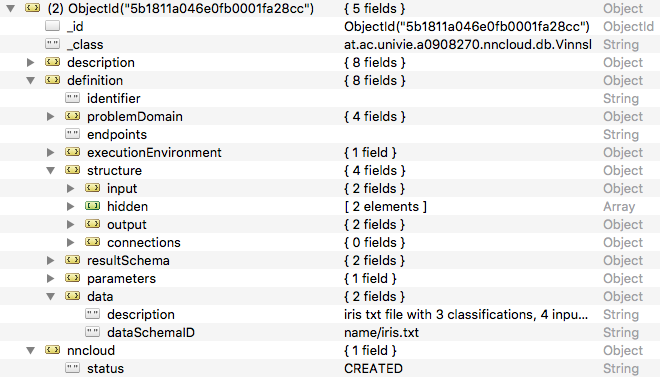
\includegraphics[width=12.00000cm]{images/usecase_1_datastructure}
\caption[Neural Network Datastructure visualized in the Robo3T
application \label{usecase_1_datastructure}]{Neural Network
Datastructure visualized in the Robo3T\footnotemark{} application
\label{usecase_1_datastructure}}
\end{figure}
\footnotetext{https://www.robomongo.org}

\subsection{Queue Network for
Training}\label{queue-network-for-training}

\subsubsection{Request}\label{request-2}

\begin{verbatim}
POST https://cluster.local/worker/queue/{id}
\end{verbatim}

\subsubsection{Response}\label{response-2}

\begin{verbatim}
200 OK
\end{verbatim}

\begin{figure}
\centering
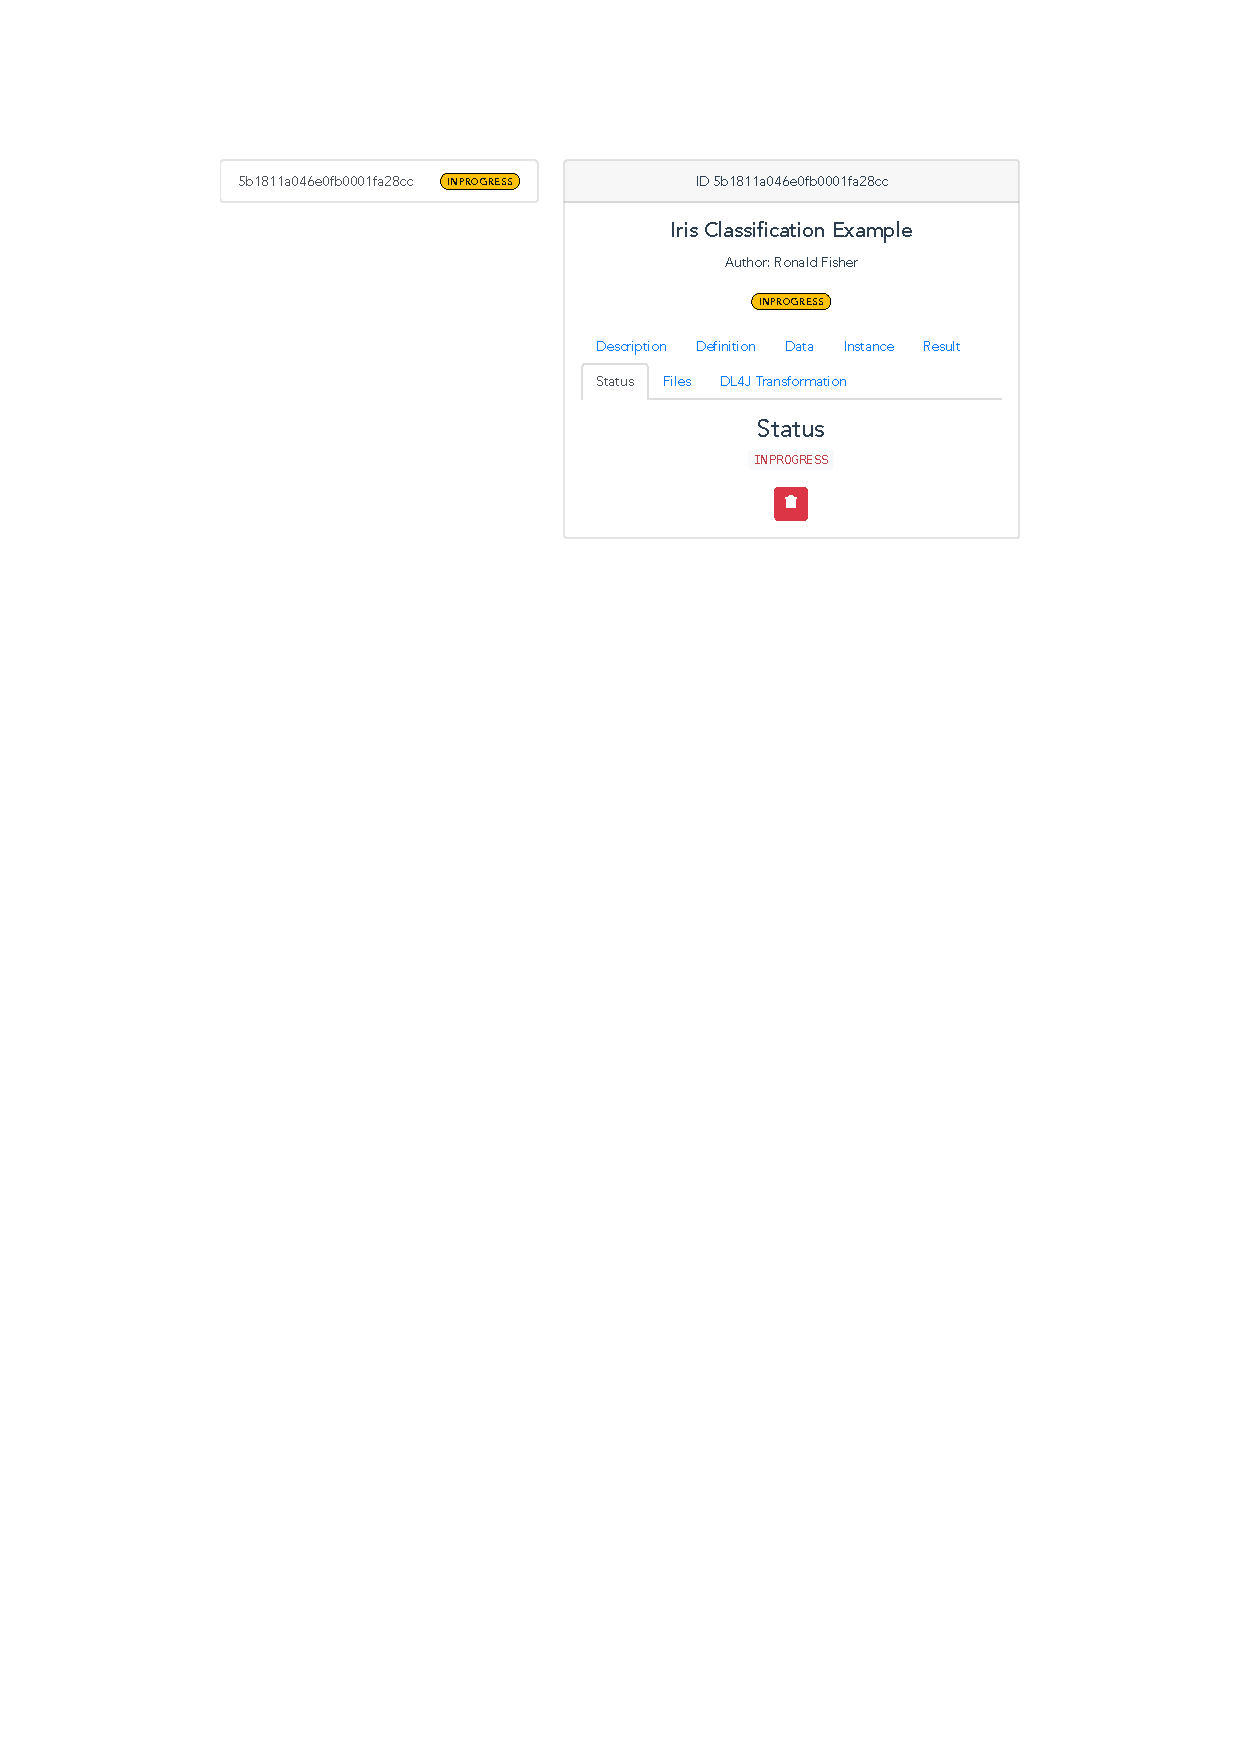
\includegraphics{images/usecase_1_ui-training}
\caption{ViNNSL NN UI shows training in progress
\label{usecase_1_ui-training}}
\end{figure}

\subsection{Training}\label{training}

During the training it is possible to open the graphical user interface
called \emph{DL4J Training UI} in a browser, that is provided with the
\emph{Deeplearning4J} package, to see the learning progress of the
neural network.

\begin{verbatim}
https://cluster.local/train/overview
\end{verbatim}

\subsubsection{DL4J Training UI}\label{dl4j-training-ui}

Figure \ref{usecase_1_ui-training_dl4j} shows the network training of
the Iris Classification. The overview tab provides general information
about network and training.

\begin{itemize}
\tightlist
\item
  Top left: score vs iteration chart - value of the loss function
\item
  Top right: model and training information
\item
  Bottom left: Ratio of parameters to updates (by layer) for all network
  weights vs.~iteration
\item
  Bottom right: Standard deviations (vs.~time) of: updates, gradients
  and activations
\end{itemize}

\cite{dl4j-traininui}

\begin{figure}
\centering
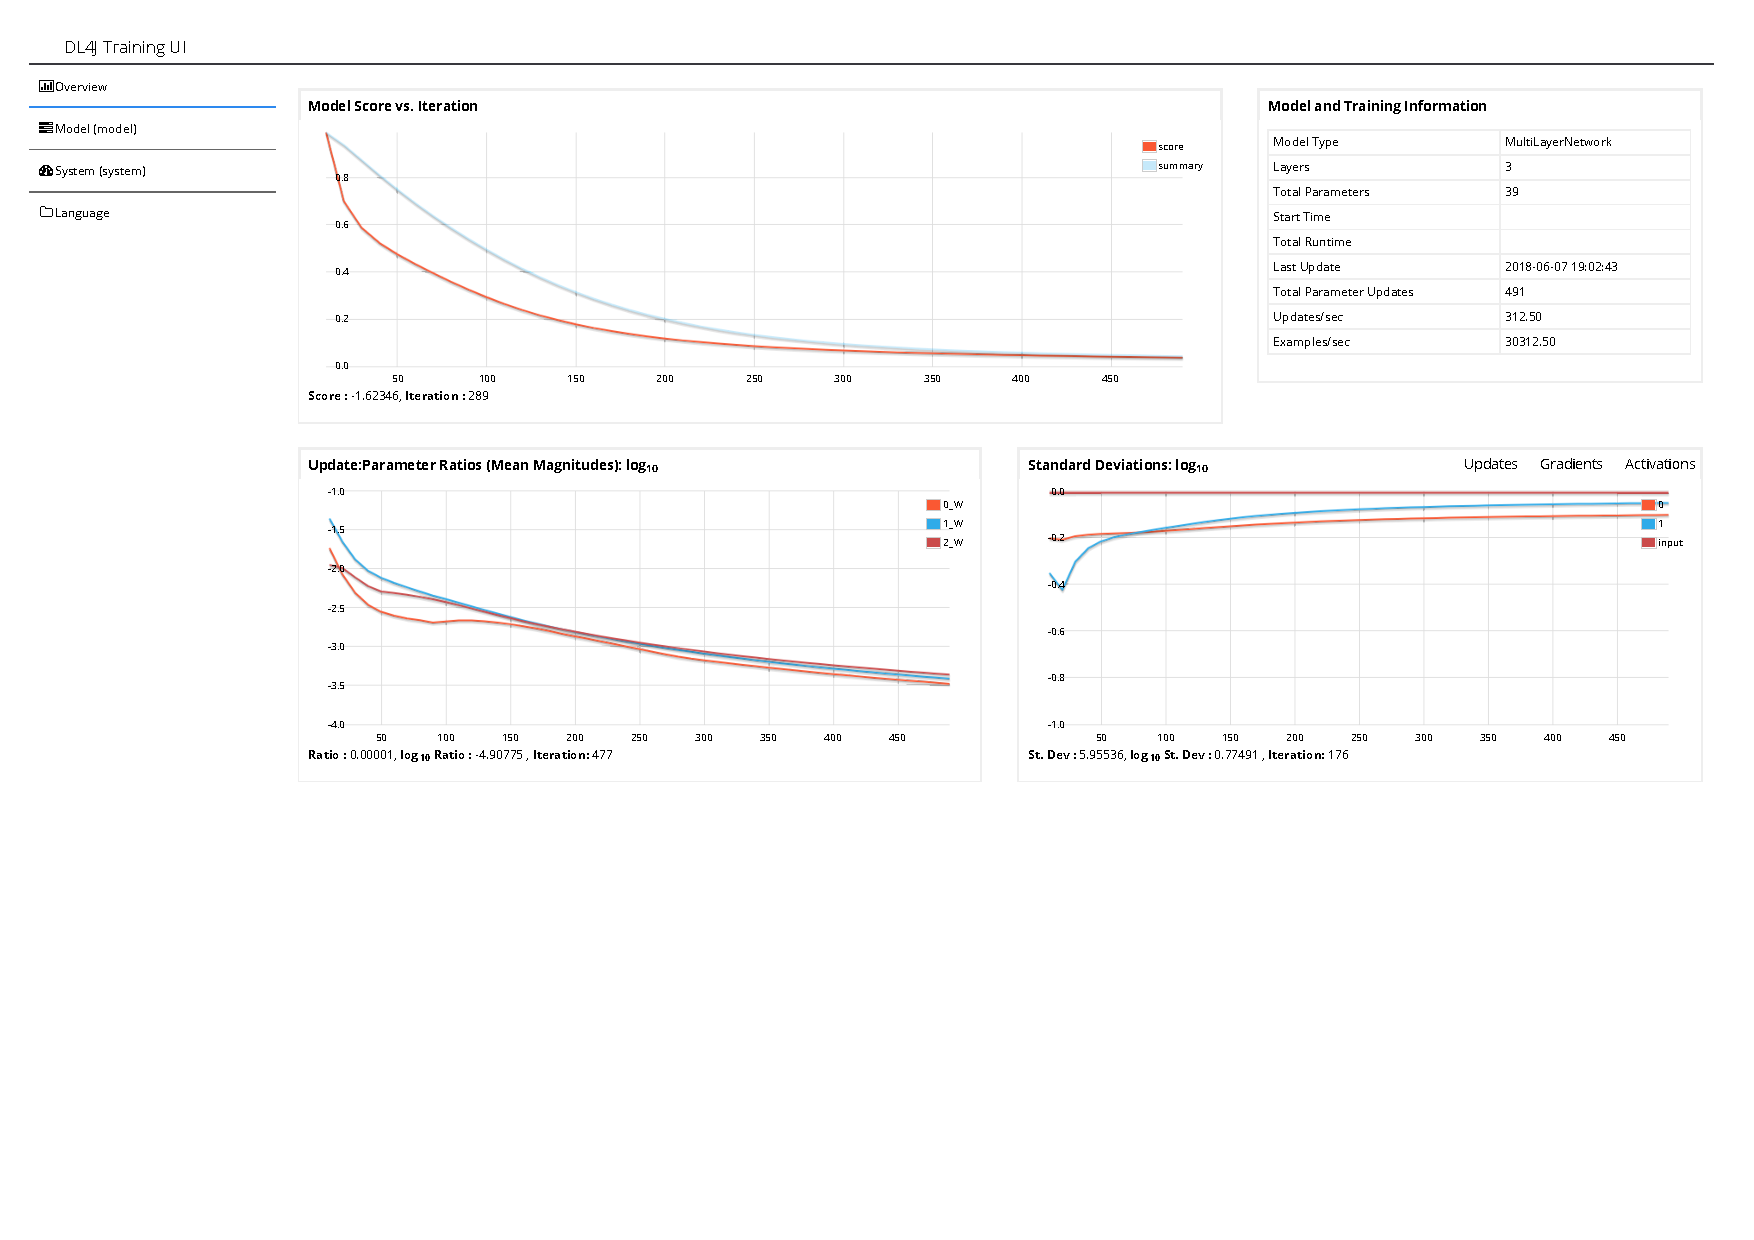
\includegraphics[width=15.00000cm]{images/usecase_1_ui-training_dl4j}
\caption{\emph{DL4J Training UI} shows training progress of Iris
Classification network \label{usecase_1_ui-training_dl4j}}
\end{figure}

The second tab provides information about the neural network layers of
the model. Information includes:

\begin{itemize}
\tightlist
\item
  Table of layer information
\item
  Layer activations over time
\item
  Histograms of parameters and updates
\item
  Learning rate vs.~time
\end{itemize}

\cite{dl4j-traininui}

\subsection{Testing}\label{testing}

Testing takes place automatically after training and evaluates the
accuracy of the trained neural network. In this case 65 percent of the
dataset is used for training and 35 percent for testing.

\subsection{Evaluate Result}\label{evaluate-result}

As soon as the training and testing process is finished a file with the
testing report is ready on the storage server. Figure
\ref{usecase_1_datastructure_finished} clarifies the updated data
structure of the neural network object. A result file with id
\texttt{5b19972052faff0001cb6bbf} was uploaded to the storage service,
the status changed to \texttt{FINISHED} and the transformed
\emph{Deeplearning4J} model representation is updated in the field
\emph{dl4jNetwork}.

\begin{figure}
\centering
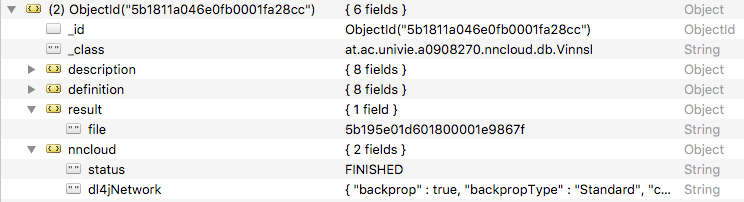
\includegraphics[width=12.00000cm]{images/usecase_1_datastructure_finished}
\caption[Neural Network Datastructure of the fninished network
visualized in the Robo3T application
\label{usecase_1_datastructure_finished}]{Neural Network Datastructure
of the fninished network visualized in the Robo3T\footnotemark{}
application \label{usecase_1_datastructure_finished}}
\end{figure}
\footnotetext{https://www.robomongo.org}

In the ViNNSL NN UI the result file can be viewed by switching to the
\emph{Data} tab and selecting \emph{See File} under the headline
\emph{Result Data}.

\begin{verbatim}
...

Examples labeled as 0 classified by model as 0: 19 times
Examples labeled as 1 classified by model as 1: 17 times
Examples labeled as 1 classified by model as 2: 2 times
Examples labeled as 2 classified by model as 2: 15 times


==========================Scores===========================================
 # of classes:    3
 Accuracy:        0.9623
 Precision:       0.9608
 Recall:          0.9649
 F1 Score:        0.9606
Precision, recall & F1: macro-averaged (equally weighted avg. of 3 classes)
===========================================================================
\end{verbatim}

By examining the result file it can be noticed that the accuracy of the
network was 96 percent. All \emph{Iris setosa} and \emph{Iris
versicolor} from the testset were recognized correctly, two \emph{Iris
virginica} were incorrectly recognized as \emph{Iris versicolor}.

\section{Hosted trained network}\label{hosted-trained-network}

TODO

\chapter{Future Work}\label{future-work}

The flexibility of the presented neural network stack opens up many
opportunities for future work and integration into already existing
frameworks and applications. This section points out a few ideas.

\section{ViNNSL Compatibility}\label{vinnsl-compatibility}

ViNNSL Compatibility is limited in the current prototype and could be
fully implemented to be fully compatible with other systems. See section
TODO for current limitations.

\section{Integration in N2Sky}\label{integration-in-n2sky}

\emph{N2Sky} features a graphical editor to design the neural network
structure and training of the model, as seen in Figure \ref{n2sky_eval}.
\emph{N2Sky} also uses the \emph{ViNNSL} language to model neural
networks and could enable to run the training process in the neural
network stack by using the provided API.

\begin{figure}
\centering
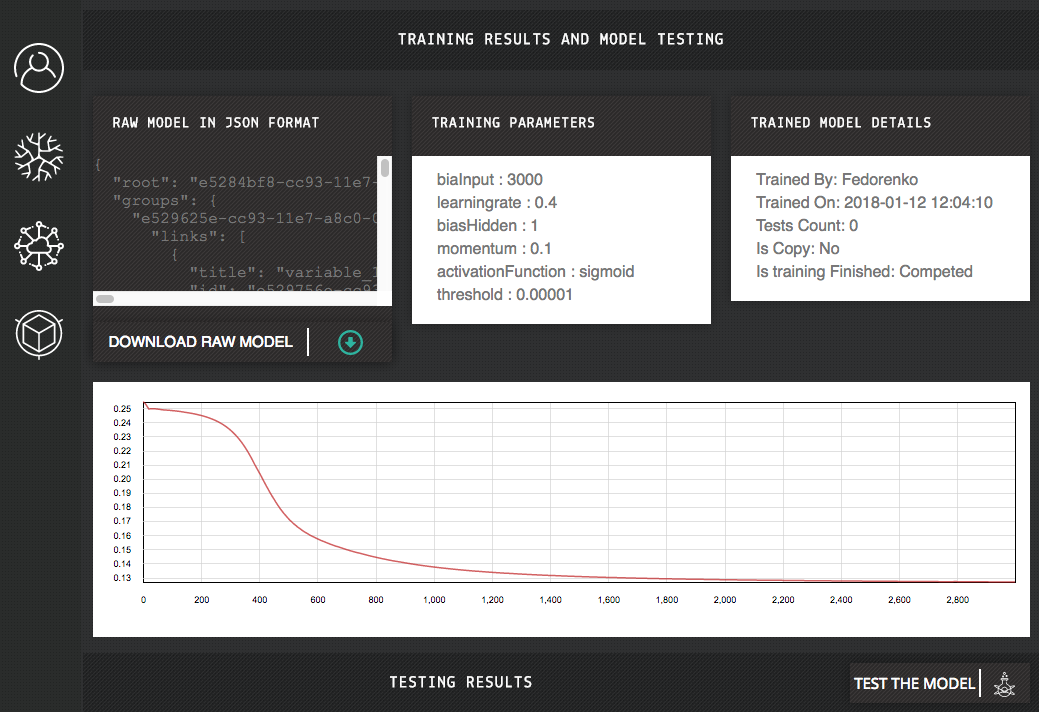
\includegraphics[width=12.00000cm]{images/n2sky_eval}
\caption{N2Sky Neural network evaluation process \cite{n2sky-2}
\label{n2sky_eval}}
\end{figure}

\section{Neural Network Backends}\label{neural-network-backends}

Presently the \emph{Deeplearning4J} platform undertakes the task of
network training. ViNNSL XML files are transformed into a
\emph{Deeplearning4J} model before training. With manageable development
effort the API could be extended to support direct import of
\emph{Deeplearning4J} models. Furthermore the Framework provides support
for Keras\footnote{https://keras.io}, a python framework that is fitted
to run on top of TensorFlow, Microsoft Cognitive Toolkit and Theano
\cite{dl4j-keras} \cite{keras}. By extending the API to enable an import
of these frameworks, demand from other target audiences could be
covered.

\section{Graphical Neural Network
Designer}\label{graphical-neural-network-designer}

The \emph{ViNNSL} XML scheme could be used to design and validate
\emph{ViNNSL} networks in a graphical editor presenting a drag\&drop
interface. Another possible function could be an integration of the
neural network stack directly into the visual designer to import and
train networks into the cluster without leaving the application.

\section{Deploy trained Models as Web
Service}\label{deploy-trained-models-as-web-service}

After the training of a neural network model is finished, a useful
functionality would be to expose the result for further predictions as a
web service. Client applications could run their requests against the
trained models to receive model predictions.

\section{Integrate into other
Platforms}\label{integrate-into-other-platforms}

There are neural network platforms on the market that could be
integrated. According to a Gartner report from February 2018,
\emph{KNIME} is currently leading in the category ``Data Science and
Machine Learning Platforms'' \cite{gartner}.

\subsection{KNIME}\label{knime}

\emph{KNIME Analytics Platform}\footnote{https://www.knime.com} is
open-source at its core\footnote{https://github.com/knime/knime-core}
and already features a \emph{Deeplearning4J} integration\footnote{https://github.com/knime/knime-dl4j}.
Figure \ref{knime} shows a screenshot of the application designing a
Multi Layer Perceptron network and exporting it to a
\emph{Deeplearning4J} model. As the application is open-source and
extensible, an option to export and train models using the presented
execution stack could be added.

\begin{figure}
\centering
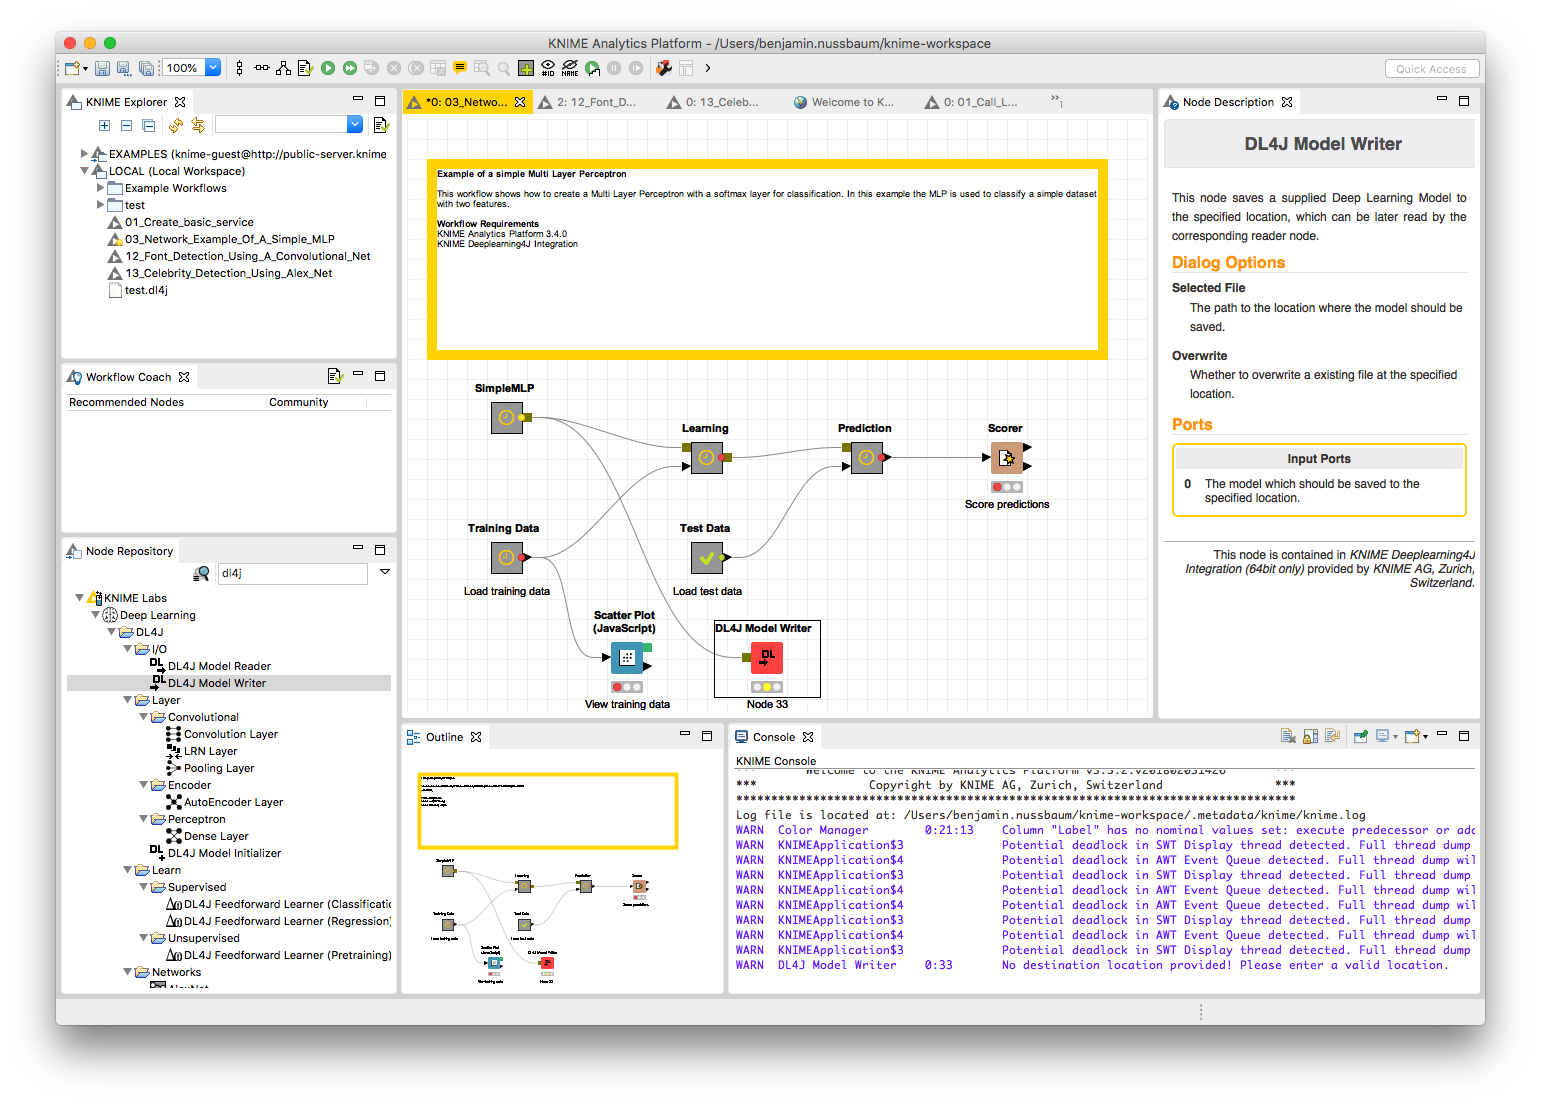
\includegraphics[width=17.00000cm]{images/knime}
\caption{Screenshot of \emph{KNIME Analytics Platform} using
\emph{Deeplearning4J} Integration \label{knime}}
\end{figure}

\section{Full featured Web
Application}\label{full-featured-web-application}

The graphical interface of the prototype provides a quick overview over
neural networks and their status, but does not cover all features
specified in the RESTful API. It could be extended to behave like a
fully featured web application that can be used as an alternative to the
API. It could also provide a functionality to integrate plugins into the
user interface.

\chapter{Conclusions}\label{conclusions}

\chapter{Acknowledgments}\label{acknowledgments}

\chapter{Dedication}\label{dedication}

\chapter{Appendices}\label{appendices}

\section{Deploy Neural Network Execution
Stack}\label{deploy-neural-network-execution-stack}

\subsection{Local Machine}\label{local-machine}

\paragraph{Prerequisites}\label{prerequisites-1}

\begin{itemize}
\tightlist
\item
  Install \texttt{kubectl} tool from:
  https://kubernetes.io/docs/tasks/tools/install-kubectl
\item
  Install \texttt{minikube} tool from:
  https://github.com/kubernetes/minikube/releases
\item
  git tool installed
\end{itemize}

\paragraph{Run minikube}\label{run-minikube}

\texttt{minikube\ start}

Starts the minikube cluster

\paragraph{Setting up}\label{setting-up}

Clone the repository

\begin{verbatim}
git clone https://github.com/a00908270/vinnsl-nn-cloud.git
cd kubernetes_config/
\end{verbatim}

\paragraph{Run Services in Cluster}\label{run-services-in-cluster}

\begin{verbatim}
# MongoDB for vinnsl-service
kubectl --context $CONTEXT create -f mongo.yaml 
# Vinnsl Service
kubectl --context $CONTEXT create -f vinnsl-service.yaml
# MongoDB for vinnsl-storage-service
kubectl --context $CONTEXT create -f mongo-storage-service.yaml
# Vinnsl Storage Service
kubectl --context $CONTEXT create -f vinnsl-storage-service.yaml
# Vinnsl NN Worker Service
kubectl --context $CONTEXT create -f vinnsl-nn-worker.yaml
# Vinnsl Frontend UI Webapp
kubectl --context $CONTEXT create -f vinnsl-nn-ui.yaml
\end{verbatim}

\paragraph{Enable and Set Up Ingress}\label{enable-and-set-up-ingress}

Sets up a proxy to make services available at the endpoint specified in
the API Specification.

\begin{verbatim}
kubectl --context $CONTEXT apply -f ingress.yaml
\end{verbatim}

\subsection{Google Cloud Instance}\label{google-cloud-instance}

This section describes how to deploy the execution stack into a
Kubernetes cluster in the Google Kubernetes Engine.

\paragraph{Prerequisites}\label{prerequisites-2}

\begin{itemize}
\item
  Google Account with activated billing or credits
\item
  \texttt{kubectl} tool on local machine installed:
  (\url{https://kubernetes.io/docs/tasks/tools/install-kubectl/\#install-kubectl})
\item
  gcloud SDK locally installed
  (\url{https://cloud.google.com/sdk/downloads})
\end{itemize}

\paragraph{Create Cluster}\label{create-cluster}

\begin{verbatim}
gcloud beta container --project "nn-cloud-201314" clusters create "cluster-1" 
--zone "us-central1-a" --username "admin" --cluster-version "1.8.8-gke.0" 
--machine-type "n1-standard-1" --image-type "COS" --disk-size "15" --scopes 
"https://www.googleapis.com/auth/compute",
"https://www.googleapis.com/auth/devstorage.read_only",
"https://www.googleapis.com/auth/logging.write",
"https://www.googleapis.com/auth/monitoring",
"https://www.googleapis.com/auth/servicecontrol",
"https://www.googleapis.com/auth/service.management.readonly",
"https://www.googleapis.com/auth/trace.append" 
--num-nodes "4" --network "default" --enable-cloud-logging 
--enable-cloud-monitoring --subnetwork "default" --addons 
HorizontalPodAutoscaling,HttpLoadBalancing,KubernetesDashboard
\end{verbatim}

\paragraph{Clone the repository}\label{clone-the-repository}

Clone the \texttt{vinnsl-nn-cloud} project and swtich into the
google-cloud folder.

\begin{verbatim}
git clone https://github.com/a00908270/vinnsl-nn-cloud.git
cd kubernetes_config/google-cloud/
\end{verbatim}

\paragraph{Run Services in Cluster}\label{run-services-in-cluster-1}

\begin{verbatim}
# MongoDB for vinnsl-service
kubectl --context $CONTEXT create -f mongo_small.yaml 
# Vinnsl Service
kubectl --context $CONTEXT create -f vinnsl-service.yaml
# MongoDB for vinnsl-storage-service
kubectl --context $CONTEXT create -f mongo-storage-service_small.yaml
# Vinnsl Storage Service
kubectl --context $CONTEXT create -f vinnsl-storage-service.yaml
# Vinnsl NN Worker Service
kubectl --context $CONTEXT create -f vinnsl-nn-worker.yaml
# Vinnsl Frontend UI Webapp
kubectl --context $CONTEXT create -f vinnsl-nn-ui.yaml
\end{verbatim}

\paragraph{Enable and Set Up Ingress}\label{enable-and-set-up-ingress-1}

Sets up a proxy to make services available at the endpoint specified in
the API Specification.

\begin{verbatim}
kubectl --context $CONTEXT apply -f ingress.yaml
\end{verbatim}

\section{}\label{section-1}
